\documentclass[a4paper,10pt]{article}

\usepackage{color}
\usepackage{xcolor}
\usepackage{tikz}
\usepackage{amsmath}
\usepackage{amssymb}
\usepackage{amsthm}
\usepackage{graphicx}
\usepackage{mathtools}
\usepackage{wrapfig}
\usepackage{multirow}
\usepackage{comment}
\usepackage{natbib}
%\usepackage{float}
\usepackage{appendix}
\usepackage{enumitem}
\usepackage{newfloat}
\usepackage{subcaption}
\usepackage[utf8]{inputenc}
\usepackage{floatrow}
\usepackage{bm}
\usepackage{hyperref}
\usepackage{tcolorbox}
\usepackage{chngcntr}
\usetikzlibrary{calc}
\usetikzlibrary{fit}
\usetikzlibrary{decorations.shapes,shapes.misc,calc, positioning, hobby, backgrounds}
\usepackage{geometry}


\tikzset{decorate sep/.style 2 args=
{decorate,decoration={shape backgrounds,shape=circle,shape size=#1,shape sep=#2}}}

\tikzset{cross/.style={cross out, draw=black, minimum size=2*(#1-\pgflinewidth), inner sep=0pt, outer sep=0pt},
%default radius will be 1pt. 
cross/.default={1pt}}

%\DeclarePairedDelimiter{\floor}{\lfloor}{\rightfloor}
%\DeclarePairedDelimiter{\ceil}{\lceil}{\rceil}

\newcommand{\denominator}{\ensuremath{n+\sum\limits_{j=1}^{h} k_{j}}}
\newcommand{\halflength}{\ensuremath{\floor{\frac{m}{2}}}}
\newcommand{\floor}[1]{\left \lfloor #1 \right \rfloor}
\newcommand{\ceil}[1]{\left \lceil #1 \right \rceil}
\newcommand{\pospart}[1]{\left( #1 \right)_{+}}
\newcommand{\negpart}[1]{\left( #1 \right)_{-}}
\newcommand{\set}[2]{\left\{ #1 \, | \, #2 \right\}}
\DeclareMathOperator*{\argmin}{\arg\!\min}

\newtheorem{theorem}{Theorem}[section]
\newtheorem{corollary}[theorem]{Corollary}
\newtheorem{lemma}[theorem]{Lemma}
\newtheorem{conjecture}[theorem]{Conjecture}

\theoremstyle{definition}
\newtheorem{definition}[theorem]{Definition}

\theoremstyle{definition}
\newtheorem{example}[theorem]{Example}

 
\theoremstyle{remark}
\newtheorem*{remark}{Remark}

\theoremstyle{definition}
\newtheorem*{note}{Note}

\DeclareFloatingEnvironment[fileext=los,
    listname={List of Example Figures},
    name=Example Figure,
    placement=tbhp,
    within=section,]{examplefigure}
    
\DeclareFloatingEnvironment[fileext=los,
    listname={List of myFigures},
    name=Figure,
    placement=tbhp,
    within=section,]{myfigure}
    
%\counterwithin{figure}{section}

\geometry{
 a4paper,
 left=20mm,
 right=20mm,
 top=20mm,
 }

\bibliographystyle{plain}

\title{\begin{Huge}\textbf{Second Year Report} \end{Huge}}
\date{\today}
\author{Thomas Lowbridge, \\ School of Mathematical Sciences, \\ University of Nottingham.}

\begin{document}


\pagestyle{empty}
{
  \renewcommand{\thispagestyle}[1]{}
  \maketitle
  \tableofcontents  
}
\clearpage
\pagestyle{plain}


\setlength{\parindent}{0pt}
\setlength{\parskip}{1em}

\newpage
\pagenumbering{arabic}


\setlength{\parindent}{0pt}
\setlength{\parskip}{1em}

\newpage
\pagenumbering{arabic}

\section{Patrolling games}
\label{Section:Patrolling games}

This chapter analyses patrolling games played between an immobile attacker, who is only present in the network for a period of time, and a mobile patroller on a graph, $Q=(N,E)$. The attacker picks a node, $i$ in $Q$, and a starting time, $\tau$, forming a strategy, $(i,\tau)$ called an attack. Their attack lasts $m$ time periods, called the attack time. Choosing a starting time to attack is equivalent to the attacker choosing an attacker interval, $I= \{ \tau,...,\tau+m-1 \}$. The patroller picks a walk, $W(t)$ in $Q$, with the choice to start at any node at time $0$. The payoff of this win-lose game (to a maximizing patroller) is $1$ if the attacker is caught and $0$ if the attacker is not caught.

If the time horizon, $\mathcal{T}=\{0,1,...,T-1 \}$, is finite then both players have a finite collection of pure strategies. However if it is infinite then both players have an infinite collection of pure strategies. In either case, by the usual application of the minimax theorem [Ref], the value of the game exists and we call it $V(Q)$, the \textit{patrol value} of $Q$ (or of $Q$,$T$,$m$). In general, both players will require the use of mixed strategies and the patrol value of $Q$ can be seen as the optimal probability of capture.

For an attack to succeed, the attacker needs to have completed their attack by the end of the game and hence, $tau \leq T-m$ (or equivalently $I \subset T$). As other attacker strategies always fail, we can safely them as they are dominated. 

These games were introduced in [Ref], and many tools were found along with complete solutions to Hamiltonian and Complete Bipartite. While only a partial solution to the Line graph was found for `long' attack times, later completed in [Ref]. 

In section [Ref] we deal with the ambiguity of the time-horizon in achieving the \textit{diametric upper bound}, $V \leq \frac{m}{\bar{d}}$, as in Lemma 9 in [Ref]. It is proposed to place potential attacks at a pair of nodes which are the furtherest apart (called diametric points) for all starting $\tau \leq T-m$, with each of these potential attacks being played with equal probability. However this mixed attack strategy achieves the diametric bound only under restrictions to the time-horizon. We provide a concrete statement about these restrictions and provide an alternative mixed attack strategy, the \textit{time-limited diametric attack strategy} to reduce them. We also extend the time-limited diametric attack strategy to a larger class of attack strategies which uses multiple nodes which form regular polygons and later irregular polygons.

As both the star graph, $S_{n}$ (Equivalent to $K_{1,n}$), and line graph, $L_{k}$, have been completely solved, we aim to incorporate both ideas into the elongated star graph, $S_{n}^{k}$ in which we elongated one of the edges in $S_{n}$ $k$ times. We partially solve this graph, in the range $m \leq 2(k+1)$ in section [Ref] by developing an extension from the time-limited attack strategy to the \textit{time-delayed attack strategy}. This attack strategy incorporates the idea of distance from the stars centre by spreading out potential attacks in time.

The time-delayed attack strategy is further extended, as we deal with more general star graphs, where all edges are possibly elongated. We finally introduce the idea of connecting the centres of generalised star graphs to form more complex graphs, with some partial solutions found by node simplification and decomposition.


\subsection{Issue and correction of the diametric bound}
\label{Section:Issue and correction of the diametric bound}
We now state Lemma 9 in \cite{Alpern2011} as the diametric bound, the attackers bound by attacking randomly throughout time at the diametric nodes.

\begin{lemma}[Diametric bound]
$V \leq \max \left\{ \frac{1}{2},\frac{m}{\raisebox{-0.5ex}{$\scriptstyle 2 \bar{d}$}} \right\}$, guaranteed by the diametric attack.
\end{lemma}

We will now look at an issue with the diametric bound when $\bar{d} < m \leq 2 \bar{d}$, so we are dealing with the bound $V \leq \frac{m}{\raisebox{-0.5ex}{$\scriptstyle 2 \bar{d}$}}$. The result of the lemma states with ambiguity that this holds for large $m$ and $T$, however the results are used for smaller $T$ such as in Theorem 16 in \citep{Alpern2011}. We will analyse this issue of `large' $T$,  and present a more concrete conclusion on conditions for which $T$ must take in order to use this bound. We will then present an altered diametric attack, which can further help to reduce the conditions on $T$ for the same bound.

The diametric attack has the attacker start at two diametrical nodes with equal probability and then choosing a starting attack time, $\tau=0,1...,T-m$ again with equal probability. Hence it can be thought of as the attacker making $2(T-m+1)$ attacks each with equal probability. To see how the patroller can do against this attacking strategy, we can consider a simple oscillatory strategy, going back and forth between the diametrical nodes, and see how many potential attacks are captured.

\begin{example}[Issue with the diametric bound]
Consider the game $(Q=L_{5},T=20,m=6)$ so $m=6 >\bar{d}=4$, then under the diametric attack the attacker has $30$ attacks, starting at $0,...,14$ at nodes $1$ and $5$. If the patroller oscillates between diametric points they capture
$1+5+6+6+4=22$ attacks out of $2(20-6+1)=30$ attacks, for a capture chance of $V=\frac{11}{15}$, which is greater than diametric bound $\frac{3}{4}$.
\end{example}

We could now consider delaying the patroller initially to get a better number of attacks, e.g. delaying in the counter example to leave at time $2$ instead of $0$ gives $3+6+6+6+2=23$. In fact it can be shown that it is best for the patroller to delay themselves till time $m-\bar{d}-1$ and then perform the oscillation between the diametric nodes (see appendix \ref{Appendix:Proof of diametric waiting time}.

This means the patroller will capture, by oscillating,

\begin{align*}
&\underbrace{m-\bar{d}}_{\text{Waiting initially}} + \underbrace{\pospart{m \times \left( M +1 \right)}}_{\text{Visits which get exactly } m \text{ attacks}} \\
&+ \underbrace{\pospart{T- \left( m-1 + \left(M +1 \right) \bar{d} \right)}+\pospart{T- \left( m-1 + \left(M +2 \right) \bar{d} \right)}}_{\text{Penultimate and final node visits}} 
\end{align*}

Where, $M=\floor{\frac{T-2m+1}{\bar{d}}}$, is the number of nodes after the two initial visits getting exactly $m$ of the potential attacks, an exact derivation of this formula is left to appendix \ref{Appendix:Proof of diametric waiting time}.

The key point is that the upper bound given by the diametric attack is dependent on $T$. An example is given in Figure \ref{Figure:Example of upper bound achieved by diametric attack} which shows that for some $T$ as in Lemma \ref{Lemma:Condition on time horizon for diametric bound to hold} and as the finite time horizon becomes infinite the corrected bound reaches the suggested bound in \cite{Alpern2011}.

\begin{lemma}[Condition on $T$ for bound to hold]
\label{Lemma:Condition on time horizon for diametric bound to hold}
When $T=m-1+(k+1)\bar{d}$ for some $k \in \mathbb{N}_{0}$ then the diametric bound holds. Furthermore as $T \rightarrow \infty$ then the diametric bound holds and moreover the errors are maximal when $T=2m-1+k\bar{d}$ for some $k \in \mathbb{N}_{0}$ with an error, inversely proportional to the time horizon, explicitly $\frac{m\bar{d}-(m-\bar{d})^{2}}{2\bar{d}(m+(k+1)\bar{d})}=\mathcal{O}(\frac{1}{T})$
\end{lemma}

For proof see Appendix \ref{Appendix:Proof of conditions on T for diametric attack}.

\begin{myfigure}
\begin{center}
% Created by tikzDevice version 0.10.1 on 2018-06-27 15:09:52
% !TEX encoding = UTF-8 Unicode
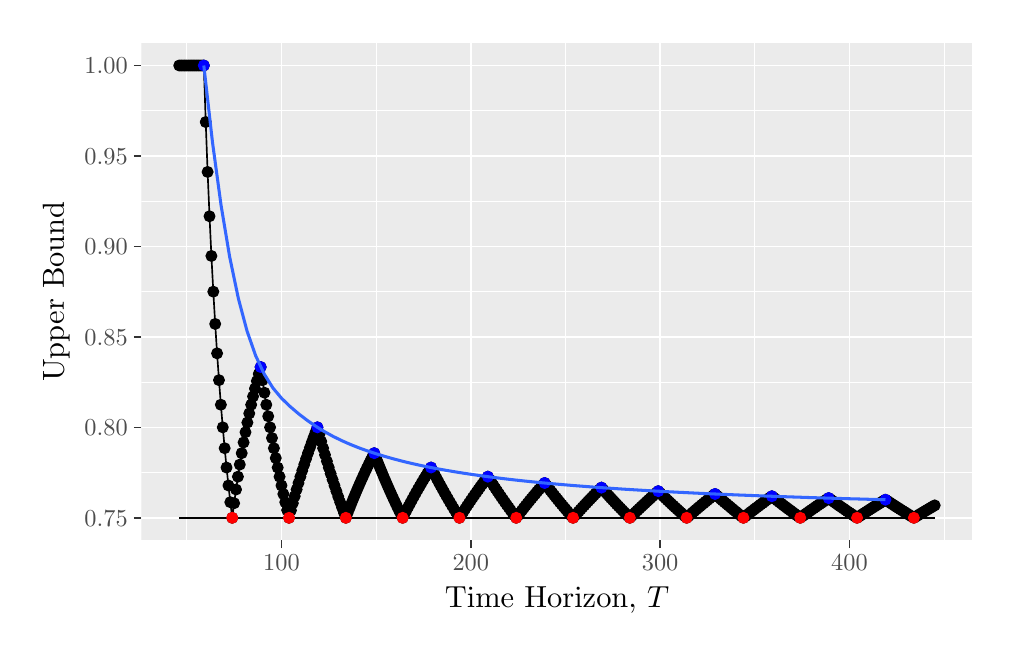
\begin{tikzpicture}[x=1pt,y=1pt]
\definecolor{fillColor}{RGB}{255,255,255}
\path[use as bounding box,fill=fillColor,fill opacity=0.00] (0,0) rectangle (346.90,216.81);
\begin{scope}
\path[clip] (  0.00,  0.00) rectangle (346.90,216.81);
\definecolor{drawColor}{RGB}{255,255,255}
\definecolor{fillColor}{RGB}{255,255,255}

\path[draw=drawColor,line width= 0.6pt,line join=round,line cap=round,fill=fillColor] (  0.00,  0.00) rectangle (346.90,216.81);
\end{scope}
\begin{scope}
\path[clip] ( 41.11, 31.53) rectangle (341.40,211.31);
\definecolor{fillColor}{gray}{0.92}

\path[fill=fillColor] ( 41.11, 31.53) rectangle (341.40,211.31);
\definecolor{drawColor}{RGB}{255,255,255}

\path[draw=drawColor,line width= 0.3pt,line join=round] ( 41.11, 56.05) --
	(341.40, 56.05);

\path[draw=drawColor,line width= 0.3pt,line join=round] ( 41.11, 88.73) --
	(341.40, 88.73);

\path[draw=drawColor,line width= 0.3pt,line join=round] ( 41.11,121.42) --
	(341.40,121.42);

\path[draw=drawColor,line width= 0.3pt,line join=round] ( 41.11,154.11) --
	(341.40,154.11);

\path[draw=drawColor,line width= 0.3pt,line join=round] ( 41.11,186.79) --
	(341.40,186.79);

\path[draw=drawColor,line width= 0.3pt,line join=round] ( 57.50, 31.53) --
	( 57.50,211.31);

\path[draw=drawColor,line width= 0.3pt,line join=round] (125.91, 31.53) --
	(125.91,211.31);

\path[draw=drawColor,line width= 0.3pt,line join=round] (194.33, 31.53) --
	(194.33,211.31);

\path[draw=drawColor,line width= 0.3pt,line join=round] (262.75, 31.53) --
	(262.75,211.31);

\path[draw=drawColor,line width= 0.3pt,line join=round] (331.17, 31.53) --
	(331.17,211.31);

\path[draw=drawColor,line width= 0.6pt,line join=round] ( 41.11, 39.70) --
	(341.40, 39.70);

\path[draw=drawColor,line width= 0.6pt,line join=round] ( 41.11, 72.39) --
	(341.40, 72.39);

\path[draw=drawColor,line width= 0.6pt,line join=round] ( 41.11,105.08) --
	(341.40,105.08);

\path[draw=drawColor,line width= 0.6pt,line join=round] ( 41.11,137.76) --
	(341.40,137.76);

\path[draw=drawColor,line width= 0.6pt,line join=round] ( 41.11,170.45) --
	(341.40,170.45);

\path[draw=drawColor,line width= 0.6pt,line join=round] ( 41.11,203.14) --
	(341.40,203.14);

\path[draw=drawColor,line width= 0.6pt,line join=round] ( 91.71, 31.53) --
	( 91.71,211.31);

\path[draw=drawColor,line width= 0.6pt,line join=round] (160.12, 31.53) --
	(160.12,211.31);

\path[draw=drawColor,line width= 0.6pt,line join=round] (228.54, 31.53) --
	(228.54,211.31);

\path[draw=drawColor,line width= 0.6pt,line join=round] (296.96, 31.53) --
	(296.96,211.31);
\definecolor{drawColor}{RGB}{0,0,0}
\definecolor{fillColor}{RGB}{0,0,0}

\path[draw=drawColor,line width= 0.4pt,line join=round,line cap=round,fill=fillColor] ( 54.76,203.14) circle (  1.96);

\path[draw=drawColor,line width= 0.4pt,line join=round,line cap=round,fill=fillColor] ( 55.44,203.14) circle (  1.96);

\path[draw=drawColor,line width= 0.4pt,line join=round,line cap=round,fill=fillColor] ( 56.13,203.14) circle (  1.96);

\path[draw=drawColor,line width= 0.4pt,line join=round,line cap=round,fill=fillColor] ( 56.81,203.14) circle (  1.96);

\path[draw=drawColor,line width= 0.4pt,line join=round,line cap=round,fill=fillColor] ( 57.50,203.14) circle (  1.96);

\path[draw=drawColor,line width= 0.4pt,line join=round,line cap=round,fill=fillColor] ( 58.18,203.14) circle (  1.96);

\path[draw=drawColor,line width= 0.4pt,line join=round,line cap=round,fill=fillColor] ( 58.87,203.14) circle (  1.96);

\path[draw=drawColor,line width= 0.4pt,line join=round,line cap=round,fill=fillColor] ( 59.55,203.14) circle (  1.96);

\path[draw=drawColor,line width= 0.4pt,line join=round,line cap=round,fill=fillColor] ( 60.23,203.14) circle (  1.96);

\path[draw=drawColor,line width= 0.4pt,line join=round,line cap=round,fill=fillColor] ( 60.92,203.14) circle (  1.96);

\path[draw=drawColor,line width= 0.4pt,line join=round,line cap=round,fill=fillColor] ( 61.60,203.14) circle (  1.96);

\path[draw=drawColor,line width= 0.4pt,line join=round,line cap=round,fill=fillColor] ( 62.29,203.14) circle (  1.96);

\path[draw=drawColor,line width= 0.4pt,line join=round,line cap=round,fill=fillColor] ( 62.97,203.14) circle (  1.96);

\path[draw=drawColor,line width= 0.4pt,line join=round,line cap=round,fill=fillColor] ( 63.65,203.14) circle (  1.96);

\path[draw=drawColor,line width= 0.4pt,line join=round,line cap=round,fill=fillColor] ( 64.34,182.71) circle (  1.96);

\path[draw=drawColor,line width= 0.4pt,line join=round,line cap=round,fill=fillColor] ( 65.02,164.68) circle (  1.96);

\path[draw=drawColor,line width= 0.4pt,line join=round,line cap=round,fill=fillColor] ( 65.71,148.66) circle (  1.96);

\path[draw=drawColor,line width= 0.4pt,line join=round,line cap=round,fill=fillColor] ( 66.39,134.32) circle (  1.96);

\path[draw=drawColor,line width= 0.4pt,line join=round,line cap=round,fill=fillColor] ( 67.08,121.42) circle (  1.96);

\path[draw=drawColor,line width= 0.4pt,line join=round,line cap=round,fill=fillColor] ( 67.76,109.75) circle (  1.96);

\path[draw=drawColor,line width= 0.4pt,line join=round,line cap=round,fill=fillColor] ( 68.44, 99.13) circle (  1.96);

\path[draw=drawColor,line width= 0.4pt,line join=round,line cap=round,fill=fillColor] ( 69.13, 89.44) circle (  1.96);

\path[draw=drawColor,line width= 0.4pt,line join=round,line cap=round,fill=fillColor] ( 69.81, 80.56) circle (  1.96);

\path[draw=drawColor,line width= 0.4pt,line join=round,line cap=round,fill=fillColor] ( 70.50, 72.39) circle (  1.96);

\path[draw=drawColor,line width= 0.4pt,line join=round,line cap=round,fill=fillColor] ( 71.18, 64.85) circle (  1.96);

\path[draw=drawColor,line width= 0.4pt,line join=round,line cap=round,fill=fillColor] ( 71.86, 57.86) circle (  1.96);

\path[draw=drawColor,line width= 0.4pt,line join=round,line cap=round,fill=fillColor] ( 72.55, 51.38) circle (  1.96);

\path[draw=drawColor,line width= 0.4pt,line join=round,line cap=round,fill=fillColor] ( 73.23, 45.34) circle (  1.96);

\path[draw=drawColor,line width= 0.4pt,line join=round,line cap=round,fill=fillColor] ( 73.92, 39.70) circle (  1.96);

\path[draw=drawColor,line width= 0.4pt,line join=round,line cap=round,fill=fillColor] ( 74.60, 44.97) circle (  1.96);

\path[draw=drawColor,line width= 0.4pt,line join=round,line cap=round,fill=fillColor] ( 75.29, 49.92) circle (  1.96);

\path[draw=drawColor,line width= 0.4pt,line join=round,line cap=round,fill=fillColor] ( 75.97, 54.56) circle (  1.96);

\path[draw=drawColor,line width= 0.4pt,line join=round,line cap=round,fill=fillColor] ( 76.65, 58.93) circle (  1.96);

\path[draw=drawColor,line width= 0.4pt,line join=round,line cap=round,fill=fillColor] ( 77.34, 63.05) circle (  1.96);

\path[draw=drawColor,line width= 0.4pt,line join=round,line cap=round,fill=fillColor] ( 78.02, 66.94) circle (  1.96);

\path[draw=drawColor,line width= 0.4pt,line join=round,line cap=round,fill=fillColor] ( 78.71, 70.62) circle (  1.96);

\path[draw=drawColor,line width= 0.4pt,line join=round,line cap=round,fill=fillColor] ( 79.39, 74.11) circle (  1.96);

\path[draw=drawColor,line width= 0.4pt,line join=round,line cap=round,fill=fillColor] ( 80.07, 77.42) circle (  1.96);

\path[draw=drawColor,line width= 0.4pt,line join=round,line cap=round,fill=fillColor] ( 80.76, 80.56) circle (  1.96);

\path[draw=drawColor,line width= 0.4pt,line join=round,line cap=round,fill=fillColor] ( 81.44, 83.55) circle (  1.96);

\path[draw=drawColor,line width= 0.4pt,line join=round,line cap=round,fill=fillColor] ( 82.13, 86.40) circle (  1.96);

\path[draw=drawColor,line width= 0.4pt,line join=round,line cap=round,fill=fillColor] ( 82.81, 89.11) circle (  1.96);

\path[draw=drawColor,line width= 0.4pt,line join=round,line cap=round,fill=fillColor] ( 83.50, 91.70) circle (  1.96);

\path[draw=drawColor,line width= 0.4pt,line join=round,line cap=round,fill=fillColor] ( 84.18, 94.18) circle (  1.96);

\path[draw=drawColor,line width= 0.4pt,line join=round,line cap=round,fill=fillColor] ( 84.86, 89.44) circle (  1.96);

\path[draw=drawColor,line width= 0.4pt,line join=round,line cap=round,fill=fillColor] ( 85.55, 84.91) circle (  1.96);

\path[draw=drawColor,line width= 0.4pt,line join=round,line cap=round,fill=fillColor] ( 86.23, 80.56) circle (  1.96);

\path[draw=drawColor,line width= 0.4pt,line join=round,line cap=round,fill=fillColor] ( 86.92, 76.39) circle (  1.96);

\path[draw=drawColor,line width= 0.4pt,line join=round,line cap=round,fill=fillColor] ( 87.60, 72.39) circle (  1.96);

\path[draw=drawColor,line width= 0.4pt,line join=round,line cap=round,fill=fillColor] ( 88.28, 68.54) circle (  1.96);

\path[draw=drawColor,line width= 0.4pt,line join=round,line cap=round,fill=fillColor] ( 88.97, 64.85) circle (  1.96);

\path[draw=drawColor,line width= 0.4pt,line join=round,line cap=round,fill=fillColor] ( 89.65, 61.29) circle (  1.96);

\path[draw=drawColor,line width= 0.4pt,line join=round,line cap=round,fill=fillColor] ( 90.34, 57.86) circle (  1.96);

\path[draw=drawColor,line width= 0.4pt,line join=round,line cap=round,fill=fillColor] ( 91.02, 54.56) circle (  1.96);

\path[draw=drawColor,line width= 0.4pt,line join=round,line cap=round,fill=fillColor] ( 91.71, 51.38) circle (  1.96);

\path[draw=drawColor,line width= 0.4pt,line join=round,line cap=round,fill=fillColor] ( 92.39, 48.30) circle (  1.96);

\path[draw=drawColor,line width= 0.4pt,line join=round,line cap=round,fill=fillColor] ( 93.07, 45.34) circle (  1.96);

\path[draw=drawColor,line width= 0.4pt,line join=round,line cap=round,fill=fillColor] ( 93.76, 42.47) circle (  1.96);

\path[draw=drawColor,line width= 0.4pt,line join=round,line cap=round,fill=fillColor] ( 94.44, 39.70) circle (  1.96);

\path[draw=drawColor,line width= 0.4pt,line join=round,line cap=round,fill=fillColor] ( 95.13, 42.38) circle (  1.96);

\path[draw=drawColor,line width= 0.4pt,line join=round,line cap=round,fill=fillColor] ( 95.81, 44.97) circle (  1.96);

\path[draw=drawColor,line width= 0.4pt,line join=round,line cap=round,fill=fillColor] ( 96.49, 47.49) circle (  1.96);

\path[draw=drawColor,line width= 0.4pt,line join=round,line cap=round,fill=fillColor] ( 97.18, 49.92) circle (  1.96);

\path[draw=drawColor,line width= 0.4pt,line join=round,line cap=round,fill=fillColor] ( 97.86, 52.27) circle (  1.96);

\path[draw=drawColor,line width= 0.4pt,line join=round,line cap=round,fill=fillColor] ( 98.55, 54.56) circle (  1.96);

\path[draw=drawColor,line width= 0.4pt,line join=round,line cap=round,fill=fillColor] ( 99.23, 56.78) circle (  1.96);

\path[draw=drawColor,line width= 0.4pt,line join=round,line cap=round,fill=fillColor] ( 99.92, 58.93) circle (  1.96);

\path[draw=drawColor,line width= 0.4pt,line join=round,line cap=round,fill=fillColor] (100.60, 61.02) circle (  1.96);

\path[draw=drawColor,line width= 0.4pt,line join=round,line cap=round,fill=fillColor] (101.28, 63.05) circle (  1.96);

\path[draw=drawColor,line width= 0.4pt,line join=round,line cap=round,fill=fillColor] (101.97, 65.02) circle (  1.96);

\path[draw=drawColor,line width= 0.4pt,line join=round,line cap=round,fill=fillColor] (102.65, 66.94) circle (  1.96);

\path[draw=drawColor,line width= 0.4pt,line join=round,line cap=round,fill=fillColor] (103.34, 68.81) circle (  1.96);

\path[draw=drawColor,line width= 0.4pt,line join=round,line cap=round,fill=fillColor] (104.02, 70.62) circle (  1.96);

\path[draw=drawColor,line width= 0.4pt,line join=round,line cap=round,fill=fillColor] (104.70, 72.39) circle (  1.96);

\path[draw=drawColor,line width= 0.4pt,line join=round,line cap=round,fill=fillColor] (105.39, 69.81) circle (  1.96);

\path[draw=drawColor,line width= 0.4pt,line join=round,line cap=round,fill=fillColor] (106.07, 67.30) circle (  1.96);

\path[draw=drawColor,line width= 0.4pt,line join=round,line cap=round,fill=fillColor] (106.76, 64.85) circle (  1.96);

\path[draw=drawColor,line width= 0.4pt,line join=round,line cap=round,fill=fillColor] (107.44, 62.46) circle (  1.96);

\path[draw=drawColor,line width= 0.4pt,line join=round,line cap=round,fill=fillColor] (108.13, 60.13) circle (  1.96);

\path[draw=drawColor,line width= 0.4pt,line join=round,line cap=round,fill=fillColor] (108.81, 57.86) circle (  1.96);

\path[draw=drawColor,line width= 0.4pt,line join=round,line cap=round,fill=fillColor] (109.49, 55.65) circle (  1.96);

\path[draw=drawColor,line width= 0.4pt,line join=round,line cap=round,fill=fillColor] (110.18, 53.49) circle (  1.96);

\path[draw=drawColor,line width= 0.4pt,line join=round,line cap=round,fill=fillColor] (110.86, 51.38) circle (  1.96);

\path[draw=drawColor,line width= 0.4pt,line join=round,line cap=round,fill=fillColor] (111.55, 49.32) circle (  1.96);

\path[draw=drawColor,line width= 0.4pt,line join=round,line cap=round,fill=fillColor] (112.23, 47.30) circle (  1.96);

\path[draw=drawColor,line width= 0.4pt,line join=round,line cap=round,fill=fillColor] (112.92, 45.34) circle (  1.96);

\path[draw=drawColor,line width= 0.4pt,line join=round,line cap=round,fill=fillColor] (113.60, 43.42) circle (  1.96);

\path[draw=drawColor,line width= 0.4pt,line join=round,line cap=round,fill=fillColor] (114.28, 41.54) circle (  1.96);

\path[draw=drawColor,line width= 0.4pt,line join=round,line cap=round,fill=fillColor] (114.97, 39.70) circle (  1.96);

\path[draw=drawColor,line width= 0.4pt,line join=round,line cap=round,fill=fillColor] (115.65, 41.50) circle (  1.96);

\path[draw=drawColor,line width= 0.4pt,line join=round,line cap=round,fill=fillColor] (116.34, 43.26) circle (  1.96);

\path[draw=drawColor,line width= 0.4pt,line join=round,line cap=round,fill=fillColor] (117.02, 44.97) circle (  1.96);

\path[draw=drawColor,line width= 0.4pt,line join=round,line cap=round,fill=fillColor] (117.70, 46.66) circle (  1.96);

\path[draw=drawColor,line width= 0.4pt,line join=round,line cap=round,fill=fillColor] (118.39, 48.30) circle (  1.96);

\path[draw=drawColor,line width= 0.4pt,line join=round,line cap=round,fill=fillColor] (119.07, 49.92) circle (  1.96);

\path[draw=drawColor,line width= 0.4pt,line join=round,line cap=round,fill=fillColor] (119.76, 51.50) circle (  1.96);

\path[draw=drawColor,line width= 0.4pt,line join=round,line cap=round,fill=fillColor] (120.44, 53.04) circle (  1.96);

\path[draw=drawColor,line width= 0.4pt,line join=round,line cap=round,fill=fillColor] (121.13, 54.56) circle (  1.96);

\path[draw=drawColor,line width= 0.4pt,line join=round,line cap=round,fill=fillColor] (121.81, 56.05) circle (  1.96);

\path[draw=drawColor,line width= 0.4pt,line join=round,line cap=round,fill=fillColor] (122.49, 57.50) circle (  1.96);

\path[draw=drawColor,line width= 0.4pt,line join=round,line cap=round,fill=fillColor] (123.18, 58.93) circle (  1.96);

\path[draw=drawColor,line width= 0.4pt,line join=round,line cap=round,fill=fillColor] (123.86, 60.33) circle (  1.96);

\path[draw=drawColor,line width= 0.4pt,line join=round,line cap=round,fill=fillColor] (124.55, 61.70) circle (  1.96);

\path[draw=drawColor,line width= 0.4pt,line join=round,line cap=round,fill=fillColor] (125.23, 63.05) circle (  1.96);

\path[draw=drawColor,line width= 0.4pt,line join=round,line cap=round,fill=fillColor] (125.91, 61.29) circle (  1.96);

\path[draw=drawColor,line width= 0.4pt,line join=round,line cap=round,fill=fillColor] (126.60, 59.56) circle (  1.96);

\path[draw=drawColor,line width= 0.4pt,line join=round,line cap=round,fill=fillColor] (127.28, 57.86) circle (  1.96);

\path[draw=drawColor,line width= 0.4pt,line join=round,line cap=round,fill=fillColor] (127.97, 56.20) circle (  1.96);

\path[draw=drawColor,line width= 0.4pt,line join=round,line cap=round,fill=fillColor] (128.65, 54.56) circle (  1.96);

\path[draw=drawColor,line width= 0.4pt,line join=round,line cap=round,fill=fillColor] (129.34, 52.95) circle (  1.96);

\path[draw=drawColor,line width= 0.4pt,line join=round,line cap=round,fill=fillColor] (130.02, 51.38) circle (  1.96);

\path[draw=drawColor,line width= 0.4pt,line join=round,line cap=round,fill=fillColor] (130.70, 49.83) circle (  1.96);

\path[draw=drawColor,line width= 0.4pt,line join=round,line cap=round,fill=fillColor] (131.39, 48.30) circle (  1.96);

\path[draw=drawColor,line width= 0.4pt,line join=round,line cap=round,fill=fillColor] (132.07, 46.81) circle (  1.96);

\path[draw=drawColor,line width= 0.4pt,line join=round,line cap=round,fill=fillColor] (132.76, 45.34) circle (  1.96);

\path[draw=drawColor,line width= 0.4pt,line join=round,line cap=round,fill=fillColor] (133.44, 43.89) circle (  1.96);

\path[draw=drawColor,line width= 0.4pt,line join=round,line cap=round,fill=fillColor] (134.12, 42.47) circle (  1.96);

\path[draw=drawColor,line width= 0.4pt,line join=round,line cap=round,fill=fillColor] (134.81, 41.08) circle (  1.96);

\path[draw=drawColor,line width= 0.4pt,line join=round,line cap=round,fill=fillColor] (135.49, 39.70) circle (  1.96);

\path[draw=drawColor,line width= 0.4pt,line join=round,line cap=round,fill=fillColor] (136.18, 41.05) circle (  1.96);

\path[draw=drawColor,line width= 0.4pt,line join=round,line cap=round,fill=fillColor] (136.86, 42.38) circle (  1.96);

\path[draw=drawColor,line width= 0.4pt,line join=round,line cap=round,fill=fillColor] (137.55, 43.69) circle (  1.96);

\path[draw=drawColor,line width= 0.4pt,line join=round,line cap=round,fill=fillColor] (138.23, 44.97) circle (  1.96);

\path[draw=drawColor,line width= 0.4pt,line join=round,line cap=round,fill=fillColor] (138.91, 46.24) circle (  1.96);

\path[draw=drawColor,line width= 0.4pt,line join=round,line cap=round,fill=fillColor] (139.60, 47.49) circle (  1.96);

\path[draw=drawColor,line width= 0.4pt,line join=round,line cap=round,fill=fillColor] (140.28, 48.71) circle (  1.96);

\path[draw=drawColor,line width= 0.4pt,line join=round,line cap=round,fill=fillColor] (140.97, 49.92) circle (  1.96);

\path[draw=drawColor,line width= 0.4pt,line join=round,line cap=round,fill=fillColor] (141.65, 51.10) circle (  1.96);

\path[draw=drawColor,line width= 0.4pt,line join=round,line cap=round,fill=fillColor] (142.33, 52.27) circle (  1.96);

\path[draw=drawColor,line width= 0.4pt,line join=round,line cap=round,fill=fillColor] (143.02, 53.43) circle (  1.96);

\path[draw=drawColor,line width= 0.4pt,line join=round,line cap=round,fill=fillColor] (143.70, 54.56) circle (  1.96);

\path[draw=drawColor,line width= 0.4pt,line join=round,line cap=round,fill=fillColor] (144.39, 55.68) circle (  1.96);

\path[draw=drawColor,line width= 0.4pt,line join=round,line cap=round,fill=fillColor] (145.07, 56.78) circle (  1.96);

\path[draw=drawColor,line width= 0.4pt,line join=round,line cap=round,fill=fillColor] (145.76, 57.86) circle (  1.96);

\path[draw=drawColor,line width= 0.4pt,line join=round,line cap=round,fill=fillColor] (146.44, 56.53) circle (  1.96);

\path[draw=drawColor,line width= 0.4pt,line join=round,line cap=round,fill=fillColor] (147.12, 55.21) circle (  1.96);

\path[draw=drawColor,line width= 0.4pt,line join=round,line cap=round,fill=fillColor] (147.81, 53.91) circle (  1.96);

\path[draw=drawColor,line width= 0.4pt,line join=round,line cap=round,fill=fillColor] (148.49, 52.64) circle (  1.96);

\path[draw=drawColor,line width= 0.4pt,line join=round,line cap=round,fill=fillColor] (149.18, 51.38) circle (  1.96);

\path[draw=drawColor,line width= 0.4pt,line join=round,line cap=round,fill=fillColor] (149.86, 50.13) circle (  1.96);

\path[draw=drawColor,line width= 0.4pt,line join=round,line cap=round,fill=fillColor] (150.54, 48.91) circle (  1.96);

\path[draw=drawColor,line width= 0.4pt,line join=round,line cap=round,fill=fillColor] (151.23, 47.70) circle (  1.96);

\path[draw=drawColor,line width= 0.4pt,line join=round,line cap=round,fill=fillColor] (151.91, 46.51) circle (  1.96);

\path[draw=drawColor,line width= 0.4pt,line join=round,line cap=round,fill=fillColor] (152.60, 45.34) circle (  1.96);

\path[draw=drawColor,line width= 0.4pt,line join=round,line cap=round,fill=fillColor] (153.28, 44.18) circle (  1.96);

\path[draw=drawColor,line width= 0.4pt,line join=round,line cap=round,fill=fillColor] (153.97, 43.04) circle (  1.96);

\path[draw=drawColor,line width= 0.4pt,line join=round,line cap=round,fill=fillColor] (154.65, 41.91) circle (  1.96);

\path[draw=drawColor,line width= 0.4pt,line join=round,line cap=round,fill=fillColor] (155.33, 40.80) circle (  1.96);

\path[draw=drawColor,line width= 0.4pt,line join=round,line cap=round,fill=fillColor] (156.02, 39.70) circle (  1.96);

\path[draw=drawColor,line width= 0.4pt,line join=round,line cap=round,fill=fillColor] (156.70, 40.78) circle (  1.96);

\path[draw=drawColor,line width= 0.4pt,line join=round,line cap=round,fill=fillColor] (157.39, 41.85) circle (  1.96);

\path[draw=drawColor,line width= 0.4pt,line join=round,line cap=round,fill=fillColor] (158.07, 42.91) circle (  1.96);

\path[draw=drawColor,line width= 0.4pt,line join=round,line cap=round,fill=fillColor] (158.75, 43.95) circle (  1.96);

\path[draw=drawColor,line width= 0.4pt,line join=round,line cap=round,fill=fillColor] (159.44, 44.97) circle (  1.96);

\path[draw=drawColor,line width= 0.4pt,line join=round,line cap=round,fill=fillColor] (160.12, 45.99) circle (  1.96);

\path[draw=drawColor,line width= 0.4pt,line join=round,line cap=round,fill=fillColor] (160.81, 46.99) circle (  1.96);

\path[draw=drawColor,line width= 0.4pt,line join=round,line cap=round,fill=fillColor] (161.49, 47.98) circle (  1.96);

\path[draw=drawColor,line width= 0.4pt,line join=round,line cap=round,fill=fillColor] (162.18, 48.95) circle (  1.96);

\path[draw=drawColor,line width= 0.4pt,line join=round,line cap=round,fill=fillColor] (162.86, 49.92) circle (  1.96);

\path[draw=drawColor,line width= 0.4pt,line join=round,line cap=round,fill=fillColor] (163.54, 50.87) circle (  1.96);

\path[draw=drawColor,line width= 0.4pt,line join=round,line cap=round,fill=fillColor] (164.23, 51.81) circle (  1.96);

\path[draw=drawColor,line width= 0.4pt,line join=round,line cap=round,fill=fillColor] (164.91, 52.74) circle (  1.96);

\path[draw=drawColor,line width= 0.4pt,line join=round,line cap=round,fill=fillColor] (165.60, 53.65) circle (  1.96);

\path[draw=drawColor,line width= 0.4pt,line join=round,line cap=round,fill=fillColor] (166.28, 54.56) circle (  1.96);

\path[draw=drawColor,line width= 0.4pt,line join=round,line cap=round,fill=fillColor] (166.97, 53.49) circle (  1.96);

\path[draw=drawColor,line width= 0.4pt,line join=round,line cap=round,fill=fillColor] (167.65, 52.43) circle (  1.96);

\path[draw=drawColor,line width= 0.4pt,line join=round,line cap=round,fill=fillColor] (168.33, 51.38) circle (  1.96);

\path[draw=drawColor,line width= 0.4pt,line join=round,line cap=round,fill=fillColor] (169.02, 50.34) circle (  1.96);

\path[draw=drawColor,line width= 0.4pt,line join=round,line cap=round,fill=fillColor] (169.70, 49.32) circle (  1.96);

\path[draw=drawColor,line width= 0.4pt,line join=round,line cap=round,fill=fillColor] (170.39, 48.30) circle (  1.96);

\path[draw=drawColor,line width= 0.4pt,line join=round,line cap=round,fill=fillColor] (171.07, 47.30) circle (  1.96);

\path[draw=drawColor,line width= 0.4pt,line join=round,line cap=round,fill=fillColor] (171.75, 46.32) circle (  1.96);

\path[draw=drawColor,line width= 0.4pt,line join=round,line cap=round,fill=fillColor] (172.44, 45.34) circle (  1.96);

\path[draw=drawColor,line width= 0.4pt,line join=round,line cap=round,fill=fillColor] (173.12, 44.37) circle (  1.96);

\path[draw=drawColor,line width= 0.4pt,line join=round,line cap=round,fill=fillColor] (173.81, 43.42) circle (  1.96);

\path[draw=drawColor,line width= 0.4pt,line join=round,line cap=round,fill=fillColor] (174.49, 42.47) circle (  1.96);

\path[draw=drawColor,line width= 0.4pt,line join=round,line cap=round,fill=fillColor] (175.18, 41.54) circle (  1.96);

\path[draw=drawColor,line width= 0.4pt,line join=round,line cap=round,fill=fillColor] (175.86, 40.62) circle (  1.96);

\path[draw=drawColor,line width= 0.4pt,line join=round,line cap=round,fill=fillColor] (176.54, 39.70) circle (  1.96);

\path[draw=drawColor,line width= 0.4pt,line join=round,line cap=round,fill=fillColor] (177.23, 40.61) circle (  1.96);

\path[draw=drawColor,line width= 0.4pt,line join=round,line cap=round,fill=fillColor] (177.91, 41.50) circle (  1.96);

\path[draw=drawColor,line width= 0.4pt,line join=round,line cap=round,fill=fillColor] (178.60, 42.38) circle (  1.96);

\path[draw=drawColor,line width= 0.4pt,line join=round,line cap=round,fill=fillColor] (179.28, 43.26) circle (  1.96);

\path[draw=drawColor,line width= 0.4pt,line join=round,line cap=round,fill=fillColor] (179.96, 44.12) circle (  1.96);

\path[draw=drawColor,line width= 0.4pt,line join=round,line cap=round,fill=fillColor] (180.65, 44.97) circle (  1.96);

\path[draw=drawColor,line width= 0.4pt,line join=round,line cap=round,fill=fillColor] (181.33, 45.82) circle (  1.96);

\path[draw=drawColor,line width= 0.4pt,line join=round,line cap=round,fill=fillColor] (182.02, 46.66) circle (  1.96);

\path[draw=drawColor,line width= 0.4pt,line join=round,line cap=round,fill=fillColor] (182.70, 47.49) circle (  1.96);

\path[draw=drawColor,line width= 0.4pt,line join=round,line cap=round,fill=fillColor] (183.39, 48.30) circle (  1.96);

\path[draw=drawColor,line width= 0.4pt,line join=round,line cap=round,fill=fillColor] (184.07, 49.12) circle (  1.96);

\path[draw=drawColor,line width= 0.4pt,line join=round,line cap=round,fill=fillColor] (184.75, 49.92) circle (  1.96);

\path[draw=drawColor,line width= 0.4pt,line join=round,line cap=round,fill=fillColor] (185.44, 50.71) circle (  1.96);

\path[draw=drawColor,line width= 0.4pt,line join=round,line cap=round,fill=fillColor] (186.12, 51.50) circle (  1.96);

\path[draw=drawColor,line width= 0.4pt,line join=round,line cap=round,fill=fillColor] (186.81, 52.27) circle (  1.96);

\path[draw=drawColor,line width= 0.4pt,line join=round,line cap=round,fill=fillColor] (187.49, 51.38) circle (  1.96);

\path[draw=drawColor,line width= 0.4pt,line join=round,line cap=round,fill=fillColor] (188.17, 50.49) circle (  1.96);

\path[draw=drawColor,line width= 0.4pt,line join=round,line cap=round,fill=fillColor] (188.86, 49.61) circle (  1.96);

\path[draw=drawColor,line width= 0.4pt,line join=round,line cap=round,fill=fillColor] (189.54, 48.74) circle (  1.96);

\path[draw=drawColor,line width= 0.4pt,line join=round,line cap=round,fill=fillColor] (190.23, 47.87) circle (  1.96);

\path[draw=drawColor,line width= 0.4pt,line join=round,line cap=round,fill=fillColor] (190.91, 47.02) circle (  1.96);

\path[draw=drawColor,line width= 0.4pt,line join=round,line cap=round,fill=fillColor] (191.60, 46.18) circle (  1.96);

\path[draw=drawColor,line width= 0.4pt,line join=round,line cap=round,fill=fillColor] (192.28, 45.34) circle (  1.96);

\path[draw=drawColor,line width= 0.4pt,line join=round,line cap=round,fill=fillColor] (192.96, 44.51) circle (  1.96);

\path[draw=drawColor,line width= 0.4pt,line join=round,line cap=round,fill=fillColor] (193.65, 43.69) circle (  1.96);

\path[draw=drawColor,line width= 0.4pt,line join=round,line cap=round,fill=fillColor] (194.33, 42.88) circle (  1.96);

\path[draw=drawColor,line width= 0.4pt,line join=round,line cap=round,fill=fillColor] (195.02, 42.07) circle (  1.96);

\path[draw=drawColor,line width= 0.4pt,line join=round,line cap=round,fill=fillColor] (195.70, 41.27) circle (  1.96);

\path[draw=drawColor,line width= 0.4pt,line join=round,line cap=round,fill=fillColor] (196.38, 40.48) circle (  1.96);

\path[draw=drawColor,line width= 0.4pt,line join=round,line cap=round,fill=fillColor] (197.07, 39.70) circle (  1.96);

\path[draw=drawColor,line width= 0.4pt,line join=round,line cap=round,fill=fillColor] (197.75, 40.48) circle (  1.96);

\path[draw=drawColor,line width= 0.4pt,line join=round,line cap=round,fill=fillColor] (198.44, 41.24) circle (  1.96);

\path[draw=drawColor,line width= 0.4pt,line join=round,line cap=round,fill=fillColor] (199.12, 42.00) circle (  1.96);

\path[draw=drawColor,line width= 0.4pt,line join=round,line cap=round,fill=fillColor] (199.81, 42.76) circle (  1.96);

\path[draw=drawColor,line width= 0.4pt,line join=round,line cap=round,fill=fillColor] (200.49, 43.50) circle (  1.96);

\path[draw=drawColor,line width= 0.4pt,line join=round,line cap=round,fill=fillColor] (201.17, 44.24) circle (  1.96);

\path[draw=drawColor,line width= 0.4pt,line join=round,line cap=round,fill=fillColor] (201.86, 44.97) circle (  1.96);

\path[draw=drawColor,line width= 0.4pt,line join=round,line cap=round,fill=fillColor] (202.54, 45.70) circle (  1.96);

\path[draw=drawColor,line width= 0.4pt,line join=round,line cap=round,fill=fillColor] (203.23, 46.42) circle (  1.96);

\path[draw=drawColor,line width= 0.4pt,line join=round,line cap=round,fill=fillColor] (203.91, 47.13) circle (  1.96);

\path[draw=drawColor,line width= 0.4pt,line join=round,line cap=round,fill=fillColor] (204.59, 47.84) circle (  1.96);

\path[draw=drawColor,line width= 0.4pt,line join=round,line cap=round,fill=fillColor] (205.28, 48.54) circle (  1.96);

\path[draw=drawColor,line width= 0.4pt,line join=round,line cap=round,fill=fillColor] (205.96, 49.23) circle (  1.96);

\path[draw=drawColor,line width= 0.4pt,line join=round,line cap=round,fill=fillColor] (206.65, 49.92) circle (  1.96);

\path[draw=drawColor,line width= 0.4pt,line join=round,line cap=round,fill=fillColor] (207.33, 50.60) circle (  1.96);

\path[draw=drawColor,line width= 0.4pt,line join=round,line cap=round,fill=fillColor] (208.02, 49.83) circle (  1.96);

\path[draw=drawColor,line width= 0.4pt,line join=round,line cap=round,fill=fillColor] (208.70, 49.06) circle (  1.96);

\path[draw=drawColor,line width= 0.4pt,line join=round,line cap=round,fill=fillColor] (209.38, 48.30) circle (  1.96);

\path[draw=drawColor,line width= 0.4pt,line join=round,line cap=round,fill=fillColor] (210.07, 47.55) circle (  1.96);

\path[draw=drawColor,line width= 0.4pt,line join=round,line cap=round,fill=fillColor] (210.75, 46.81) circle (  1.96);

\path[draw=drawColor,line width= 0.4pt,line join=round,line cap=round,fill=fillColor] (211.44, 46.07) circle (  1.96);

\path[draw=drawColor,line width= 0.4pt,line join=round,line cap=round,fill=fillColor] (212.12, 45.34) circle (  1.96);

\path[draw=drawColor,line width= 0.4pt,line join=round,line cap=round,fill=fillColor] (212.80, 44.61) circle (  1.96);

\path[draw=drawColor,line width= 0.4pt,line join=round,line cap=round,fill=fillColor] (213.49, 43.89) circle (  1.96);

\path[draw=drawColor,line width= 0.4pt,line join=round,line cap=round,fill=fillColor] (214.17, 43.18) circle (  1.96);

\path[draw=drawColor,line width= 0.4pt,line join=round,line cap=round,fill=fillColor] (214.86, 42.47) circle (  1.96);

\path[draw=drawColor,line width= 0.4pt,line join=round,line cap=round,fill=fillColor] (215.54, 41.77) circle (  1.96);

\path[draw=drawColor,line width= 0.4pt,line join=round,line cap=round,fill=fillColor] (216.23, 41.08) circle (  1.96);

\path[draw=drawColor,line width= 0.4pt,line join=round,line cap=round,fill=fillColor] (216.91, 40.39) circle (  1.96);

\path[draw=drawColor,line width= 0.4pt,line join=round,line cap=round,fill=fillColor] (217.59, 39.70) circle (  1.96);

\path[draw=drawColor,line width= 0.4pt,line join=round,line cap=round,fill=fillColor] (218.28, 40.38) circle (  1.96);

\path[draw=drawColor,line width= 0.4pt,line join=round,line cap=round,fill=fillColor] (218.96, 41.05) circle (  1.96);

\path[draw=drawColor,line width= 0.4pt,line join=round,line cap=round,fill=fillColor] (219.65, 41.72) circle (  1.96);

\path[draw=drawColor,line width= 0.4pt,line join=round,line cap=round,fill=fillColor] (220.33, 42.38) circle (  1.96);

\path[draw=drawColor,line width= 0.4pt,line join=round,line cap=round,fill=fillColor] (221.02, 43.04) circle (  1.96);

\path[draw=drawColor,line width= 0.4pt,line join=round,line cap=round,fill=fillColor] (221.70, 43.69) circle (  1.96);

\path[draw=drawColor,line width= 0.4pt,line join=round,line cap=round,fill=fillColor] (222.38, 44.33) circle (  1.96);

\path[draw=drawColor,line width= 0.4pt,line join=round,line cap=round,fill=fillColor] (223.07, 44.97) circle (  1.96);

\path[draw=drawColor,line width= 0.4pt,line join=round,line cap=round,fill=fillColor] (223.75, 45.61) circle (  1.96);

\path[draw=drawColor,line width= 0.4pt,line join=round,line cap=round,fill=fillColor] (224.44, 46.24) circle (  1.96);

\path[draw=drawColor,line width= 0.4pt,line join=round,line cap=round,fill=fillColor] (225.12, 46.87) circle (  1.96);

\path[draw=drawColor,line width= 0.4pt,line join=round,line cap=round,fill=fillColor] (225.80, 47.49) circle (  1.96);

\path[draw=drawColor,line width= 0.4pt,line join=round,line cap=round,fill=fillColor] (226.49, 48.10) circle (  1.96);

\path[draw=drawColor,line width= 0.4pt,line join=round,line cap=round,fill=fillColor] (227.17, 48.71) circle (  1.96);

\path[draw=drawColor,line width= 0.4pt,line join=round,line cap=round,fill=fillColor] (227.86, 49.32) circle (  1.96);

\path[draw=drawColor,line width= 0.4pt,line join=round,line cap=round,fill=fillColor] (228.54, 48.64) circle (  1.96);

\path[draw=drawColor,line width= 0.4pt,line join=round,line cap=round,fill=fillColor] (229.23, 47.97) circle (  1.96);

\path[draw=drawColor,line width= 0.4pt,line join=round,line cap=round,fill=fillColor] (229.91, 47.30) circle (  1.96);

\path[draw=drawColor,line width= 0.4pt,line join=round,line cap=round,fill=fillColor] (230.59, 46.64) circle (  1.96);

\path[draw=drawColor,line width= 0.4pt,line join=round,line cap=round,fill=fillColor] (231.28, 45.99) circle (  1.96);

\path[draw=drawColor,line width= 0.4pt,line join=round,line cap=round,fill=fillColor] (231.96, 45.34) circle (  1.96);

\path[draw=drawColor,line width= 0.4pt,line join=round,line cap=round,fill=fillColor] (232.65, 44.69) circle (  1.96);

\path[draw=drawColor,line width= 0.4pt,line join=round,line cap=round,fill=fillColor] (233.33, 44.05) circle (  1.96);

\path[draw=drawColor,line width= 0.4pt,line join=round,line cap=round,fill=fillColor] (234.01, 43.42) circle (  1.96);

\path[draw=drawColor,line width= 0.4pt,line join=round,line cap=round,fill=fillColor] (234.70, 42.79) circle (  1.96);

\path[draw=drawColor,line width= 0.4pt,line join=round,line cap=round,fill=fillColor] (235.38, 42.16) circle (  1.96);

\path[draw=drawColor,line width= 0.4pt,line join=round,line cap=round,fill=fillColor] (236.07, 41.54) circle (  1.96);

\path[draw=drawColor,line width= 0.4pt,line join=round,line cap=round,fill=fillColor] (236.75, 40.92) circle (  1.96);

\path[draw=drawColor,line width= 0.4pt,line join=round,line cap=round,fill=fillColor] (237.44, 40.31) circle (  1.96);

\path[draw=drawColor,line width= 0.4pt,line join=round,line cap=round,fill=fillColor] (238.12, 39.70) circle (  1.96);

\path[draw=drawColor,line width= 0.4pt,line join=round,line cap=round,fill=fillColor] (238.80, 40.31) circle (  1.96);

\path[draw=drawColor,line width= 0.4pt,line join=round,line cap=round,fill=fillColor] (239.49, 40.90) circle (  1.96);

\path[draw=drawColor,line width= 0.4pt,line join=round,line cap=round,fill=fillColor] (240.17, 41.50) circle (  1.96);

\path[draw=drawColor,line width= 0.4pt,line join=round,line cap=round,fill=fillColor] (240.86, 42.09) circle (  1.96);

\path[draw=drawColor,line width= 0.4pt,line join=round,line cap=round,fill=fillColor] (241.54, 42.67) circle (  1.96);

\path[draw=drawColor,line width= 0.4pt,line join=round,line cap=round,fill=fillColor] (242.22, 43.26) circle (  1.96);

\path[draw=drawColor,line width= 0.4pt,line join=round,line cap=round,fill=fillColor] (242.91, 43.83) circle (  1.96);

\path[draw=drawColor,line width= 0.4pt,line join=round,line cap=round,fill=fillColor] (243.59, 44.41) circle (  1.96);

\path[draw=drawColor,line width= 0.4pt,line join=round,line cap=round,fill=fillColor] (244.28, 44.97) circle (  1.96);

\path[draw=drawColor,line width= 0.4pt,line join=round,line cap=round,fill=fillColor] (244.96, 45.54) circle (  1.96);

\path[draw=drawColor,line width= 0.4pt,line join=round,line cap=round,fill=fillColor] (245.65, 46.10) circle (  1.96);

\path[draw=drawColor,line width= 0.4pt,line join=round,line cap=round,fill=fillColor] (246.33, 46.66) circle (  1.96);

\path[draw=drawColor,line width= 0.4pt,line join=round,line cap=round,fill=fillColor] (247.01, 47.21) circle (  1.96);

\path[draw=drawColor,line width= 0.4pt,line join=round,line cap=round,fill=fillColor] (247.70, 47.76) circle (  1.96);

\path[draw=drawColor,line width= 0.4pt,line join=round,line cap=round,fill=fillColor] (248.38, 48.30) circle (  1.96);

\path[draw=drawColor,line width= 0.4pt,line join=round,line cap=round,fill=fillColor] (249.07, 47.70) circle (  1.96);

\path[draw=drawColor,line width= 0.4pt,line join=round,line cap=round,fill=fillColor] (249.75, 47.11) circle (  1.96);

\path[draw=drawColor,line width= 0.4pt,line join=round,line cap=round,fill=fillColor] (250.43, 46.51) circle (  1.96);

\path[draw=drawColor,line width= 0.4pt,line join=round,line cap=round,fill=fillColor] (251.12, 45.92) circle (  1.96);

\path[draw=drawColor,line width= 0.4pt,line join=round,line cap=round,fill=fillColor] (251.80, 45.34) circle (  1.96);

\path[draw=drawColor,line width= 0.4pt,line join=round,line cap=round,fill=fillColor] (252.49, 44.76) circle (  1.96);

\path[draw=drawColor,line width= 0.4pt,line join=round,line cap=round,fill=fillColor] (253.17, 44.18) circle (  1.96);

\path[draw=drawColor,line width= 0.4pt,line join=round,line cap=round,fill=fillColor] (253.86, 43.61) circle (  1.96);

\path[draw=drawColor,line width= 0.4pt,line join=round,line cap=round,fill=fillColor] (254.54, 43.04) circle (  1.96);

\path[draw=drawColor,line width= 0.4pt,line join=round,line cap=round,fill=fillColor] (255.22, 42.47) circle (  1.96);

\path[draw=drawColor,line width= 0.4pt,line join=round,line cap=round,fill=fillColor] (255.91, 41.91) circle (  1.96);

\path[draw=drawColor,line width= 0.4pt,line join=round,line cap=round,fill=fillColor] (256.59, 41.35) circle (  1.96);

\path[draw=drawColor,line width= 0.4pt,line join=round,line cap=round,fill=fillColor] (257.28, 40.80) circle (  1.96);

\path[draw=drawColor,line width= 0.4pt,line join=round,line cap=round,fill=fillColor] (257.96, 40.25) circle (  1.96);

\path[draw=drawColor,line width= 0.4pt,line join=round,line cap=round,fill=fillColor] (258.64, 39.70) circle (  1.96);

\path[draw=drawColor,line width= 0.4pt,line join=round,line cap=round,fill=fillColor] (259.33, 40.25) circle (  1.96);

\path[draw=drawColor,line width= 0.4pt,line join=round,line cap=round,fill=fillColor] (260.01, 40.78) circle (  1.96);

\path[draw=drawColor,line width= 0.4pt,line join=round,line cap=round,fill=fillColor] (260.70, 41.32) circle (  1.96);

\path[draw=drawColor,line width= 0.4pt,line join=round,line cap=round,fill=fillColor] (261.38, 41.85) circle (  1.96);

\path[draw=drawColor,line width= 0.4pt,line join=round,line cap=round,fill=fillColor] (262.07, 42.38) circle (  1.96);

\path[draw=drawColor,line width= 0.4pt,line join=round,line cap=round,fill=fillColor] (262.75, 42.91) circle (  1.96);

\path[draw=drawColor,line width= 0.4pt,line join=round,line cap=round,fill=fillColor] (263.43, 43.43) circle (  1.96);

\path[draw=drawColor,line width= 0.4pt,line join=round,line cap=round,fill=fillColor] (264.12, 43.95) circle (  1.96);

\path[draw=drawColor,line width= 0.4pt,line join=round,line cap=round,fill=fillColor] (264.80, 44.46) circle (  1.96);

\path[draw=drawColor,line width= 0.4pt,line join=round,line cap=round,fill=fillColor] (265.49, 44.97) circle (  1.96);

\path[draw=drawColor,line width= 0.4pt,line join=round,line cap=round,fill=fillColor] (266.17, 45.48) circle (  1.96);

\path[draw=drawColor,line width= 0.4pt,line join=round,line cap=round,fill=fillColor] (266.85, 45.99) circle (  1.96);

\path[draw=drawColor,line width= 0.4pt,line join=round,line cap=round,fill=fillColor] (267.54, 46.49) circle (  1.96);

\path[draw=drawColor,line width= 0.4pt,line join=round,line cap=round,fill=fillColor] (268.22, 46.99) circle (  1.96);

\path[draw=drawColor,line width= 0.4pt,line join=round,line cap=round,fill=fillColor] (268.91, 47.49) circle (  1.96);

\path[draw=drawColor,line width= 0.4pt,line join=round,line cap=round,fill=fillColor] (269.59, 46.94) circle (  1.96);

\path[draw=drawColor,line width= 0.4pt,line join=round,line cap=round,fill=fillColor] (270.28, 46.40) circle (  1.96);

\path[draw=drawColor,line width= 0.4pt,line join=round,line cap=round,fill=fillColor] (270.96, 45.87) circle (  1.96);

\path[draw=drawColor,line width= 0.4pt,line join=round,line cap=round,fill=fillColor] (271.64, 45.34) circle (  1.96);

\path[draw=drawColor,line width= 0.4pt,line join=round,line cap=round,fill=fillColor] (272.33, 44.81) circle (  1.96);

\path[draw=drawColor,line width= 0.4pt,line join=round,line cap=round,fill=fillColor] (273.01, 44.28) circle (  1.96);

\path[draw=drawColor,line width= 0.4pt,line join=round,line cap=round,fill=fillColor] (273.70, 43.76) circle (  1.96);

\path[draw=drawColor,line width= 0.4pt,line join=round,line cap=round,fill=fillColor] (274.38, 43.24) circle (  1.96);

\path[draw=drawColor,line width= 0.4pt,line join=round,line cap=round,fill=fillColor] (275.07, 42.73) circle (  1.96);

\path[draw=drawColor,line width= 0.4pt,line join=round,line cap=round,fill=fillColor] (275.75, 42.22) circle (  1.96);

\path[draw=drawColor,line width= 0.4pt,line join=round,line cap=round,fill=fillColor] (276.43, 41.71) circle (  1.96);

\path[draw=drawColor,line width= 0.4pt,line join=round,line cap=round,fill=fillColor] (277.12, 41.20) circle (  1.96);

\path[draw=drawColor,line width= 0.4pt,line join=round,line cap=round,fill=fillColor] (277.80, 40.70) circle (  1.96);

\path[draw=drawColor,line width= 0.4pt,line join=round,line cap=round,fill=fillColor] (278.49, 40.20) circle (  1.96);

\path[draw=drawColor,line width= 0.4pt,line join=round,line cap=round,fill=fillColor] (279.17, 39.70) circle (  1.96);

\path[draw=drawColor,line width= 0.4pt,line join=round,line cap=round,fill=fillColor] (279.85, 40.20) circle (  1.96);

\path[draw=drawColor,line width= 0.4pt,line join=round,line cap=round,fill=fillColor] (280.54, 40.69) circle (  1.96);

\path[draw=drawColor,line width= 0.4pt,line join=round,line cap=round,fill=fillColor] (281.22, 41.17) circle (  1.96);

\path[draw=drawColor,line width= 0.4pt,line join=round,line cap=round,fill=fillColor] (281.91, 41.66) circle (  1.96);

\path[draw=drawColor,line width= 0.4pt,line join=round,line cap=round,fill=fillColor] (282.59, 42.14) circle (  1.96);

\path[draw=drawColor,line width= 0.4pt,line join=round,line cap=round,fill=fillColor] (283.28, 42.62) circle (  1.96);

\path[draw=drawColor,line width= 0.4pt,line join=round,line cap=round,fill=fillColor] (283.96, 43.10) circle (  1.96);

\path[draw=drawColor,line width= 0.4pt,line join=round,line cap=round,fill=fillColor] (284.64, 43.57) circle (  1.96);

\path[draw=drawColor,line width= 0.4pt,line join=round,line cap=round,fill=fillColor] (285.33, 44.04) circle (  1.96);

\path[draw=drawColor,line width= 0.4pt,line join=round,line cap=round,fill=fillColor] (286.01, 44.51) circle (  1.96);

\path[draw=drawColor,line width= 0.4pt,line join=round,line cap=round,fill=fillColor] (286.70, 44.97) circle (  1.96);

\path[draw=drawColor,line width= 0.4pt,line join=round,line cap=round,fill=fillColor] (287.38, 45.44) circle (  1.96);

\path[draw=drawColor,line width= 0.4pt,line join=round,line cap=round,fill=fillColor] (288.06, 45.90) circle (  1.96);

\path[draw=drawColor,line width= 0.4pt,line join=round,line cap=round,fill=fillColor] (288.75, 46.35) circle (  1.96);

\path[draw=drawColor,line width= 0.4pt,line join=round,line cap=round,fill=fillColor] (289.43, 46.81) circle (  1.96);

\path[draw=drawColor,line width= 0.4pt,line join=round,line cap=round,fill=fillColor] (290.12, 46.32) circle (  1.96);

\path[draw=drawColor,line width= 0.4pt,line join=round,line cap=round,fill=fillColor] (290.80, 45.83) circle (  1.96);

\path[draw=drawColor,line width= 0.4pt,line join=round,line cap=round,fill=fillColor] (291.49, 45.34) circle (  1.96);

\path[draw=drawColor,line width= 0.4pt,line join=round,line cap=round,fill=fillColor] (292.17, 44.85) circle (  1.96);

\path[draw=drawColor,line width= 0.4pt,line join=round,line cap=round,fill=fillColor] (292.85, 44.37) circle (  1.96);

\path[draw=drawColor,line width= 0.4pt,line join=round,line cap=round,fill=fillColor] (293.54, 43.89) circle (  1.96);

\path[draw=drawColor,line width= 0.4pt,line join=round,line cap=round,fill=fillColor] (294.22, 43.42) circle (  1.96);

\path[draw=drawColor,line width= 0.4pt,line join=round,line cap=round,fill=fillColor] (294.91, 42.94) circle (  1.96);

\path[draw=drawColor,line width= 0.4pt,line join=round,line cap=round,fill=fillColor] (295.59, 42.47) circle (  1.96);

\path[draw=drawColor,line width= 0.4pt,line join=round,line cap=round,fill=fillColor] (296.27, 42.00) circle (  1.96);

\path[draw=drawColor,line width= 0.4pt,line join=round,line cap=round,fill=fillColor] (296.96, 41.54) circle (  1.96);

\path[draw=drawColor,line width= 0.4pt,line join=round,line cap=round,fill=fillColor] (297.64, 41.08) circle (  1.96);

\path[draw=drawColor,line width= 0.4pt,line join=round,line cap=round,fill=fillColor] (298.33, 40.62) circle (  1.96);

\path[draw=drawColor,line width= 0.4pt,line join=round,line cap=round,fill=fillColor] (299.01, 40.16) circle (  1.96);

\path[draw=drawColor,line width= 0.4pt,line join=round,line cap=round,fill=fillColor] (299.70, 39.70) circle (  1.96);

\path[draw=drawColor,line width= 0.4pt,line join=round,line cap=round,fill=fillColor] (300.38, 40.16) circle (  1.96);

\path[draw=drawColor,line width= 0.4pt,line join=round,line cap=round,fill=fillColor] (301.06, 40.61) circle (  1.96);

\path[draw=drawColor,line width= 0.4pt,line join=round,line cap=round,fill=fillColor] (301.75, 41.05) circle (  1.96);

\path[draw=drawColor,line width= 0.4pt,line join=round,line cap=round,fill=fillColor] (302.43, 41.50) circle (  1.96);

\path[draw=drawColor,line width= 0.4pt,line join=round,line cap=round,fill=fillColor] (303.12, 41.94) circle (  1.96);

\path[draw=drawColor,line width= 0.4pt,line join=round,line cap=round,fill=fillColor] (303.80, 42.38) circle (  1.96);

\path[draw=drawColor,line width= 0.4pt,line join=round,line cap=round,fill=fillColor] (304.48, 42.82) circle (  1.96);

\path[draw=drawColor,line width= 0.4pt,line join=round,line cap=round,fill=fillColor] (305.17, 43.26) circle (  1.96);

\path[draw=drawColor,line width= 0.4pt,line join=round,line cap=round,fill=fillColor] (305.85, 43.69) circle (  1.96);

\path[draw=drawColor,line width= 0.4pt,line join=round,line cap=round,fill=fillColor] (306.54, 44.12) circle (  1.96);

\path[draw=drawColor,line width= 0.4pt,line join=round,line cap=round,fill=fillColor] (307.22, 44.55) circle (  1.96);

\path[draw=drawColor,line width= 0.4pt,line join=round,line cap=round,fill=fillColor] (307.91, 44.97) circle (  1.96);

\path[draw=drawColor,line width= 0.4pt,line join=round,line cap=round,fill=fillColor] (308.59, 45.40) circle (  1.96);

\path[draw=drawColor,line width= 0.4pt,line join=round,line cap=round,fill=fillColor] (309.27, 45.82) circle (  1.96);

\path[draw=drawColor,line width= 0.4pt,line join=round,line cap=round,fill=fillColor] (309.96, 46.24) circle (  1.96);

\path[draw=drawColor,line width= 0.4pt,line join=round,line cap=round,fill=fillColor] (310.64, 45.79) circle (  1.96);

\path[draw=drawColor,line width= 0.4pt,line join=round,line cap=round,fill=fillColor] (311.33, 45.34) circle (  1.96);

\path[draw=drawColor,line width= 0.4pt,line join=round,line cap=round,fill=fillColor] (312.01, 44.89) circle (  1.96);

\path[draw=drawColor,line width= 0.4pt,line join=round,line cap=round,fill=fillColor] (312.69, 44.45) circle (  1.96);

\path[draw=drawColor,line width= 0.4pt,line join=round,line cap=round,fill=fillColor] (313.38, 44.00) circle (  1.96);

\path[draw=drawColor,line width= 0.4pt,line join=round,line cap=round,fill=fillColor] (314.06, 43.56) circle (  1.96);

\path[draw=drawColor,line width= 0.4pt,line join=round,line cap=round,fill=fillColor] (314.75, 43.13) circle (  1.96);

\path[draw=drawColor,line width= 0.4pt,line join=round,line cap=round,fill=fillColor] (315.43, 42.69) circle (  1.96);

\path[draw=drawColor,line width= 0.4pt,line join=round,line cap=round,fill=fillColor] (316.12, 42.26) circle (  1.96);

\path[draw=drawColor,line width= 0.4pt,line join=round,line cap=round,fill=fillColor] (316.80, 41.83) circle (  1.96);

\path[draw=drawColor,line width= 0.4pt,line join=round,line cap=round,fill=fillColor] (317.48, 41.40) circle (  1.96);

\path[draw=drawColor,line width= 0.4pt,line join=round,line cap=round,fill=fillColor] (318.17, 40.97) circle (  1.96);

\path[draw=drawColor,line width= 0.4pt,line join=round,line cap=round,fill=fillColor] (318.85, 40.54) circle (  1.96);

\path[draw=drawColor,line width= 0.4pt,line join=round,line cap=round,fill=fillColor] (319.54, 40.12) circle (  1.96);

\path[draw=drawColor,line width= 0.4pt,line join=round,line cap=round,fill=fillColor] (320.22, 39.70) circle (  1.96);

\path[draw=drawColor,line width= 0.4pt,line join=round,line cap=round,fill=fillColor] (320.90, 40.12) circle (  1.96);

\path[draw=drawColor,line width= 0.4pt,line join=round,line cap=round,fill=fillColor] (321.59, 40.54) circle (  1.96);

\path[draw=drawColor,line width= 0.4pt,line join=round,line cap=round,fill=fillColor] (322.27, 40.95) circle (  1.96);

\path[draw=drawColor,line width= 0.4pt,line join=round,line cap=round,fill=fillColor] (322.96, 41.36) circle (  1.96);

\path[draw=drawColor,line width= 0.4pt,line join=round,line cap=round,fill=fillColor] (323.64, 41.77) circle (  1.96);

\path[draw=drawColor,line width= 0.4pt,line join=round,line cap=round,fill=fillColor] (324.33, 42.18) circle (  1.96);

\path[draw=drawColor,line width= 0.4pt,line join=round,line cap=round,fill=fillColor] (325.01, 42.58) circle (  1.96);

\path[draw=drawColor,line width= 0.4pt,line join=round,line cap=round,fill=fillColor] (325.69, 42.99) circle (  1.96);

\path[draw=drawColor,line width= 0.4pt,line join=round,line cap=round,fill=fillColor] (326.38, 43.39) circle (  1.96);

\path[draw=drawColor,line width= 0.4pt,line join=round,line cap=round,fill=fillColor] (327.06, 43.79) circle (  1.96);

\path[draw=drawColor,line width= 0.4pt,line join=round,line cap=round,fill=fillColor] (327.75, 44.19) circle (  1.96);

\path[draw=drawColor,line width= 0.6pt,line join=round] ( 54.76,203.14) --
	( 55.44,203.14) --
	( 56.13,203.14) --
	( 56.81,203.14) --
	( 57.50,203.14) --
	( 58.18,203.14) --
	( 58.87,203.14) --
	( 59.55,203.14) --
	( 60.23,203.14) --
	( 60.92,203.14) --
	( 61.60,203.14) --
	( 62.29,203.14) --
	( 62.97,203.14) --
	( 63.65,203.14) --
	( 64.34,182.71) --
	( 65.02,164.68) --
	( 65.71,148.66) --
	( 66.39,134.32) --
	( 67.08,121.42) --
	( 67.76,109.75) --
	( 68.44, 99.13) --
	( 69.13, 89.44) --
	( 69.81, 80.56) --
	( 70.50, 72.39) --
	( 71.18, 64.85) --
	( 71.86, 57.86) --
	( 72.55, 51.38) --
	( 73.23, 45.34) --
	( 73.92, 39.70) --
	( 74.60, 44.97) --
	( 75.29, 49.92) --
	( 75.97, 54.56) --
	( 76.65, 58.93) --
	( 77.34, 63.05) --
	( 78.02, 66.94) --
	( 78.71, 70.62) --
	( 79.39, 74.11) --
	( 80.07, 77.42) --
	( 80.76, 80.56) --
	( 81.44, 83.55) --
	( 82.13, 86.40) --
	( 82.81, 89.11) --
	( 83.50, 91.70) --
	( 84.18, 94.18) --
	( 84.86, 89.44) --
	( 85.55, 84.91) --
	( 86.23, 80.56) --
	( 86.92, 76.39) --
	( 87.60, 72.39) --
	( 88.28, 68.54) --
	( 88.97, 64.85) --
	( 89.65, 61.29) --
	( 90.34, 57.86) --
	( 91.02, 54.56) --
	( 91.71, 51.38) --
	( 92.39, 48.30) --
	( 93.07, 45.34) --
	( 93.76, 42.47) --
	( 94.44, 39.70) --
	( 95.13, 42.38) --
	( 95.81, 44.97) --
	( 96.49, 47.49) --
	( 97.18, 49.92) --
	( 97.86, 52.27) --
	( 98.55, 54.56) --
	( 99.23, 56.78) --
	( 99.92, 58.93) --
	(100.60, 61.02) --
	(101.28, 63.05) --
	(101.97, 65.02) --
	(102.65, 66.94) --
	(103.34, 68.81) --
	(104.02, 70.62) --
	(104.70, 72.39) --
	(105.39, 69.81) --
	(106.07, 67.30) --
	(106.76, 64.85) --
	(107.44, 62.46) --
	(108.13, 60.13) --
	(108.81, 57.86) --
	(109.49, 55.65) --
	(110.18, 53.49) --
	(110.86, 51.38) --
	(111.55, 49.32) --
	(112.23, 47.30) --
	(112.92, 45.34) --
	(113.60, 43.42) --
	(114.28, 41.54) --
	(114.97, 39.70) --
	(115.65, 41.50) --
	(116.34, 43.26) --
	(117.02, 44.97) --
	(117.70, 46.66) --
	(118.39, 48.30) --
	(119.07, 49.92) --
	(119.76, 51.50) --
	(120.44, 53.04) --
	(121.13, 54.56) --
	(121.81, 56.05) --
	(122.49, 57.50) --
	(123.18, 58.93) --
	(123.86, 60.33) --
	(124.55, 61.70) --
	(125.23, 63.05) --
	(125.91, 61.29) --
	(126.60, 59.56) --
	(127.28, 57.86) --
	(127.97, 56.20) --
	(128.65, 54.56) --
	(129.34, 52.95) --
	(130.02, 51.38) --
	(130.70, 49.83) --
	(131.39, 48.30) --
	(132.07, 46.81) --
	(132.76, 45.34) --
	(133.44, 43.89) --
	(134.12, 42.47) --
	(134.81, 41.08) --
	(135.49, 39.70) --
	(136.18, 41.05) --
	(136.86, 42.38) --
	(137.55, 43.69) --
	(138.23, 44.97) --
	(138.91, 46.24) --
	(139.60, 47.49) --
	(140.28, 48.71) --
	(140.97, 49.92) --
	(141.65, 51.10) --
	(142.33, 52.27) --
	(143.02, 53.43) --
	(143.70, 54.56) --
	(144.39, 55.68) --
	(145.07, 56.78) --
	(145.76, 57.86) --
	(146.44, 56.53) --
	(147.12, 55.21) --
	(147.81, 53.91) --
	(148.49, 52.64) --
	(149.18, 51.38) --
	(149.86, 50.13) --
	(150.54, 48.91) --
	(151.23, 47.70) --
	(151.91, 46.51) --
	(152.60, 45.34) --
	(153.28, 44.18) --
	(153.97, 43.04) --
	(154.65, 41.91) --
	(155.33, 40.80) --
	(156.02, 39.70) --
	(156.70, 40.78) --
	(157.39, 41.85) --
	(158.07, 42.91) --
	(158.75, 43.95) --
	(159.44, 44.97) --
	(160.12, 45.99) --
	(160.81, 46.99) --
	(161.49, 47.98) --
	(162.18, 48.95) --
	(162.86, 49.92) --
	(163.54, 50.87) --
	(164.23, 51.81) --
	(164.91, 52.74) --
	(165.60, 53.65) --
	(166.28, 54.56) --
	(166.97, 53.49) --
	(167.65, 52.43) --
	(168.33, 51.38) --
	(169.02, 50.34) --
	(169.70, 49.32) --
	(170.39, 48.30) --
	(171.07, 47.30) --
	(171.75, 46.32) --
	(172.44, 45.34) --
	(173.12, 44.37) --
	(173.81, 43.42) --
	(174.49, 42.47) --
	(175.18, 41.54) --
	(175.86, 40.62) --
	(176.54, 39.70) --
	(177.23, 40.61) --
	(177.91, 41.50) --
	(178.60, 42.38) --
	(179.28, 43.26) --
	(179.96, 44.12) --
	(180.65, 44.97) --
	(181.33, 45.82) --
	(182.02, 46.66) --
	(182.70, 47.49) --
	(183.39, 48.30) --
	(184.07, 49.12) --
	(184.75, 49.92) --
	(185.44, 50.71) --
	(186.12, 51.50) --
	(186.81, 52.27) --
	(187.49, 51.38) --
	(188.17, 50.49) --
	(188.86, 49.61) --
	(189.54, 48.74) --
	(190.23, 47.87) --
	(190.91, 47.02) --
	(191.60, 46.18) --
	(192.28, 45.34) --
	(192.96, 44.51) --
	(193.65, 43.69) --
	(194.33, 42.88) --
	(195.02, 42.07) --
	(195.70, 41.27) --
	(196.38, 40.48) --
	(197.07, 39.70) --
	(197.75, 40.48) --
	(198.44, 41.24) --
	(199.12, 42.00) --
	(199.81, 42.76) --
	(200.49, 43.50) --
	(201.17, 44.24) --
	(201.86, 44.97) --
	(202.54, 45.70) --
	(203.23, 46.42) --
	(203.91, 47.13) --
	(204.59, 47.84) --
	(205.28, 48.54) --
	(205.96, 49.23) --
	(206.65, 49.92) --
	(207.33, 50.60) --
	(208.02, 49.83) --
	(208.70, 49.06) --
	(209.38, 48.30) --
	(210.07, 47.55) --
	(210.75, 46.81) --
	(211.44, 46.07) --
	(212.12, 45.34) --
	(212.80, 44.61) --
	(213.49, 43.89) --
	(214.17, 43.18) --
	(214.86, 42.47) --
	(215.54, 41.77) --
	(216.23, 41.08) --
	(216.91, 40.39) --
	(217.59, 39.70) --
	(218.28, 40.38) --
	(218.96, 41.05) --
	(219.65, 41.72) --
	(220.33, 42.38) --
	(221.02, 43.04) --
	(221.70, 43.69) --
	(222.38, 44.33) --
	(223.07, 44.97) --
	(223.75, 45.61) --
	(224.44, 46.24) --
	(225.12, 46.87) --
	(225.80, 47.49) --
	(226.49, 48.10) --
	(227.17, 48.71) --
	(227.86, 49.32) --
	(228.54, 48.64) --
	(229.23, 47.97) --
	(229.91, 47.30) --
	(230.59, 46.64) --
	(231.28, 45.99) --
	(231.96, 45.34) --
	(232.65, 44.69) --
	(233.33, 44.05) --
	(234.01, 43.42) --
	(234.70, 42.79) --
	(235.38, 42.16) --
	(236.07, 41.54) --
	(236.75, 40.92) --
	(237.44, 40.31) --
	(238.12, 39.70) --
	(238.80, 40.31) --
	(239.49, 40.90) --
	(240.17, 41.50) --
	(240.86, 42.09) --
	(241.54, 42.67) --
	(242.22, 43.26) --
	(242.91, 43.83) --
	(243.59, 44.41) --
	(244.28, 44.97) --
	(244.96, 45.54) --
	(245.65, 46.10) --
	(246.33, 46.66) --
	(247.01, 47.21) --
	(247.70, 47.76) --
	(248.38, 48.30) --
	(249.07, 47.70) --
	(249.75, 47.11) --
	(250.43, 46.51) --
	(251.12, 45.92) --
	(251.80, 45.34) --
	(252.49, 44.76) --
	(253.17, 44.18) --
	(253.86, 43.61) --
	(254.54, 43.04) --
	(255.22, 42.47) --
	(255.91, 41.91) --
	(256.59, 41.35) --
	(257.28, 40.80) --
	(257.96, 40.25) --
	(258.64, 39.70) --
	(259.33, 40.25) --
	(260.01, 40.78) --
	(260.70, 41.32) --
	(261.38, 41.85) --
	(262.07, 42.38) --
	(262.75, 42.91) --
	(263.43, 43.43) --
	(264.12, 43.95) --
	(264.80, 44.46) --
	(265.49, 44.97) --
	(266.17, 45.48) --
	(266.85, 45.99) --
	(267.54, 46.49) --
	(268.22, 46.99) --
	(268.91, 47.49) --
	(269.59, 46.94) --
	(270.28, 46.40) --
	(270.96, 45.87) --
	(271.64, 45.34) --
	(272.33, 44.81) --
	(273.01, 44.28) --
	(273.70, 43.76) --
	(274.38, 43.24) --
	(275.07, 42.73) --
	(275.75, 42.22) --
	(276.43, 41.71) --
	(277.12, 41.20) --
	(277.80, 40.70) --
	(278.49, 40.20) --
	(279.17, 39.70) --
	(279.85, 40.20) --
	(280.54, 40.69) --
	(281.22, 41.17) --
	(281.91, 41.66) --
	(282.59, 42.14) --
	(283.28, 42.62) --
	(283.96, 43.10) --
	(284.64, 43.57) --
	(285.33, 44.04) --
	(286.01, 44.51) --
	(286.70, 44.97) --
	(287.38, 45.44) --
	(288.06, 45.90) --
	(288.75, 46.35) --
	(289.43, 46.81) --
	(290.12, 46.32) --
	(290.80, 45.83) --
	(291.49, 45.34) --
	(292.17, 44.85) --
	(292.85, 44.37) --
	(293.54, 43.89) --
	(294.22, 43.42) --
	(294.91, 42.94) --
	(295.59, 42.47) --
	(296.27, 42.00) --
	(296.96, 41.54) --
	(297.64, 41.08) --
	(298.33, 40.62) --
	(299.01, 40.16) --
	(299.70, 39.70) --
	(300.38, 40.16) --
	(301.06, 40.61) --
	(301.75, 41.05) --
	(302.43, 41.50) --
	(303.12, 41.94) --
	(303.80, 42.38) --
	(304.48, 42.82) --
	(305.17, 43.26) --
	(305.85, 43.69) --
	(306.54, 44.12) --
	(307.22, 44.55) --
	(307.91, 44.97) --
	(308.59, 45.40) --
	(309.27, 45.82) --
	(309.96, 46.24) --
	(310.64, 45.79) --
	(311.33, 45.34) --
	(312.01, 44.89) --
	(312.69, 44.45) --
	(313.38, 44.00) --
	(314.06, 43.56) --
	(314.75, 43.13) --
	(315.43, 42.69) --
	(316.12, 42.26) --
	(316.80, 41.83) --
	(317.48, 41.40) --
	(318.17, 40.97) --
	(318.85, 40.54) --
	(319.54, 40.12) --
	(320.22, 39.70) --
	(320.90, 40.12) --
	(321.59, 40.54) --
	(322.27, 40.95) --
	(322.96, 41.36) --
	(323.64, 41.77) --
	(324.33, 42.18) --
	(325.01, 42.58) --
	(325.69, 42.99) --
	(326.38, 43.39) --
	(327.06, 43.79) --
	(327.75, 44.19);

\path[draw=drawColor,line width= 0.6pt,line join=round] ( 54.76, 39.70) --
	( 55.44, 39.70) --
	( 56.13, 39.70) --
	( 56.81, 39.70) --
	( 57.50, 39.70) --
	( 58.18, 39.70) --
	( 58.87, 39.70) --
	( 59.55, 39.70) --
	( 60.23, 39.70) --
	( 60.92, 39.70) --
	( 61.60, 39.70) --
	( 62.29, 39.70) --
	( 62.97, 39.70) --
	( 63.65, 39.70) --
	( 64.34, 39.70) --
	( 65.02, 39.70) --
	( 65.71, 39.70) --
	( 66.39, 39.70) --
	( 67.08, 39.70) --
	( 67.76, 39.70) --
	( 68.44, 39.70) --
	( 69.13, 39.70) --
	( 69.81, 39.70) --
	( 70.50, 39.70) --
	( 71.18, 39.70) --
	( 71.86, 39.70) --
	( 72.55, 39.70) --
	( 73.23, 39.70) --
	( 73.92, 39.70) --
	( 74.60, 39.70) --
	( 75.29, 39.70) --
	( 75.97, 39.70) --
	( 76.65, 39.70) --
	( 77.34, 39.70) --
	( 78.02, 39.70) --
	( 78.71, 39.70) --
	( 79.39, 39.70) --
	( 80.07, 39.70) --
	( 80.76, 39.70) --
	( 81.44, 39.70) --
	( 82.13, 39.70) --
	( 82.81, 39.70) --
	( 83.50, 39.70) --
	( 84.18, 39.70) --
	( 84.86, 39.70) --
	( 85.55, 39.70) --
	( 86.23, 39.70) --
	( 86.92, 39.70) --
	( 87.60, 39.70) --
	( 88.28, 39.70) --
	( 88.97, 39.70) --
	( 89.65, 39.70) --
	( 90.34, 39.70) --
	( 91.02, 39.70) --
	( 91.71, 39.70) --
	( 92.39, 39.70) --
	( 93.07, 39.70) --
	( 93.76, 39.70) --
	( 94.44, 39.70) --
	( 95.13, 39.70) --
	( 95.81, 39.70) --
	( 96.49, 39.70) --
	( 97.18, 39.70) --
	( 97.86, 39.70) --
	( 98.55, 39.70) --
	( 99.23, 39.70) --
	( 99.92, 39.70) --
	(100.60, 39.70) --
	(101.28, 39.70) --
	(101.97, 39.70) --
	(102.65, 39.70) --
	(103.34, 39.70) --
	(104.02, 39.70) --
	(104.70, 39.70) --
	(105.39, 39.70) --
	(106.07, 39.70) --
	(106.76, 39.70) --
	(107.44, 39.70) --
	(108.13, 39.70) --
	(108.81, 39.70) --
	(109.49, 39.70) --
	(110.18, 39.70) --
	(110.86, 39.70) --
	(111.55, 39.70) --
	(112.23, 39.70) --
	(112.92, 39.70) --
	(113.60, 39.70) --
	(114.28, 39.70) --
	(114.97, 39.70) --
	(115.65, 39.70) --
	(116.34, 39.70) --
	(117.02, 39.70) --
	(117.70, 39.70) --
	(118.39, 39.70) --
	(119.07, 39.70) --
	(119.76, 39.70) --
	(120.44, 39.70) --
	(121.13, 39.70) --
	(121.81, 39.70) --
	(122.49, 39.70) --
	(123.18, 39.70) --
	(123.86, 39.70) --
	(124.55, 39.70) --
	(125.23, 39.70) --
	(125.91, 39.70) --
	(126.60, 39.70) --
	(127.28, 39.70) --
	(127.97, 39.70) --
	(128.65, 39.70) --
	(129.34, 39.70) --
	(130.02, 39.70) --
	(130.70, 39.70) --
	(131.39, 39.70) --
	(132.07, 39.70) --
	(132.76, 39.70) --
	(133.44, 39.70) --
	(134.12, 39.70) --
	(134.81, 39.70) --
	(135.49, 39.70) --
	(136.18, 39.70) --
	(136.86, 39.70) --
	(137.55, 39.70) --
	(138.23, 39.70) --
	(138.91, 39.70) --
	(139.60, 39.70) --
	(140.28, 39.70) --
	(140.97, 39.70) --
	(141.65, 39.70) --
	(142.33, 39.70) --
	(143.02, 39.70) --
	(143.70, 39.70) --
	(144.39, 39.70) --
	(145.07, 39.70) --
	(145.76, 39.70) --
	(146.44, 39.70) --
	(147.12, 39.70) --
	(147.81, 39.70) --
	(148.49, 39.70) --
	(149.18, 39.70) --
	(149.86, 39.70) --
	(150.54, 39.70) --
	(151.23, 39.70) --
	(151.91, 39.70) --
	(152.60, 39.70) --
	(153.28, 39.70) --
	(153.97, 39.70) --
	(154.65, 39.70) --
	(155.33, 39.70) --
	(156.02, 39.70) --
	(156.70, 39.70) --
	(157.39, 39.70) --
	(158.07, 39.70) --
	(158.75, 39.70) --
	(159.44, 39.70) --
	(160.12, 39.70) --
	(160.81, 39.70) --
	(161.49, 39.70) --
	(162.18, 39.70) --
	(162.86, 39.70) --
	(163.54, 39.70) --
	(164.23, 39.70) --
	(164.91, 39.70) --
	(165.60, 39.70) --
	(166.28, 39.70) --
	(166.97, 39.70) --
	(167.65, 39.70) --
	(168.33, 39.70) --
	(169.02, 39.70) --
	(169.70, 39.70) --
	(170.39, 39.70) --
	(171.07, 39.70) --
	(171.75, 39.70) --
	(172.44, 39.70) --
	(173.12, 39.70) --
	(173.81, 39.70) --
	(174.49, 39.70) --
	(175.18, 39.70) --
	(175.86, 39.70) --
	(176.54, 39.70) --
	(177.23, 39.70) --
	(177.91, 39.70) --
	(178.60, 39.70) --
	(179.28, 39.70) --
	(179.96, 39.70) --
	(180.65, 39.70) --
	(181.33, 39.70) --
	(182.02, 39.70) --
	(182.70, 39.70) --
	(183.39, 39.70) --
	(184.07, 39.70) --
	(184.75, 39.70) --
	(185.44, 39.70) --
	(186.12, 39.70) --
	(186.81, 39.70) --
	(187.49, 39.70) --
	(188.17, 39.70) --
	(188.86, 39.70) --
	(189.54, 39.70) --
	(190.23, 39.70) --
	(190.91, 39.70) --
	(191.60, 39.70) --
	(192.28, 39.70) --
	(192.96, 39.70) --
	(193.65, 39.70) --
	(194.33, 39.70) --
	(195.02, 39.70) --
	(195.70, 39.70) --
	(196.38, 39.70) --
	(197.07, 39.70) --
	(197.75, 39.70) --
	(198.44, 39.70) --
	(199.12, 39.70) --
	(199.81, 39.70) --
	(200.49, 39.70) --
	(201.17, 39.70) --
	(201.86, 39.70) --
	(202.54, 39.70) --
	(203.23, 39.70) --
	(203.91, 39.70) --
	(204.59, 39.70) --
	(205.28, 39.70) --
	(205.96, 39.70) --
	(206.65, 39.70) --
	(207.33, 39.70) --
	(208.02, 39.70) --
	(208.70, 39.70) --
	(209.38, 39.70) --
	(210.07, 39.70) --
	(210.75, 39.70) --
	(211.44, 39.70) --
	(212.12, 39.70) --
	(212.80, 39.70) --
	(213.49, 39.70) --
	(214.17, 39.70) --
	(214.86, 39.70) --
	(215.54, 39.70) --
	(216.23, 39.70) --
	(216.91, 39.70) --
	(217.59, 39.70) --
	(218.28, 39.70) --
	(218.96, 39.70) --
	(219.65, 39.70) --
	(220.33, 39.70) --
	(221.02, 39.70) --
	(221.70, 39.70) --
	(222.38, 39.70) --
	(223.07, 39.70) --
	(223.75, 39.70) --
	(224.44, 39.70) --
	(225.12, 39.70) --
	(225.80, 39.70) --
	(226.49, 39.70) --
	(227.17, 39.70) --
	(227.86, 39.70) --
	(228.54, 39.70) --
	(229.23, 39.70) --
	(229.91, 39.70) --
	(230.59, 39.70) --
	(231.28, 39.70) --
	(231.96, 39.70) --
	(232.65, 39.70) --
	(233.33, 39.70) --
	(234.01, 39.70) --
	(234.70, 39.70) --
	(235.38, 39.70) --
	(236.07, 39.70) --
	(236.75, 39.70) --
	(237.44, 39.70) --
	(238.12, 39.70) --
	(238.80, 39.70) --
	(239.49, 39.70) --
	(240.17, 39.70) --
	(240.86, 39.70) --
	(241.54, 39.70) --
	(242.22, 39.70) --
	(242.91, 39.70) --
	(243.59, 39.70) --
	(244.28, 39.70) --
	(244.96, 39.70) --
	(245.65, 39.70) --
	(246.33, 39.70) --
	(247.01, 39.70) --
	(247.70, 39.70) --
	(248.38, 39.70) --
	(249.07, 39.70) --
	(249.75, 39.70) --
	(250.43, 39.70) --
	(251.12, 39.70) --
	(251.80, 39.70) --
	(252.49, 39.70) --
	(253.17, 39.70) --
	(253.86, 39.70) --
	(254.54, 39.70) --
	(255.22, 39.70) --
	(255.91, 39.70) --
	(256.59, 39.70) --
	(257.28, 39.70) --
	(257.96, 39.70) --
	(258.64, 39.70) --
	(259.33, 39.70) --
	(260.01, 39.70) --
	(260.70, 39.70) --
	(261.38, 39.70) --
	(262.07, 39.70) --
	(262.75, 39.70) --
	(263.43, 39.70) --
	(264.12, 39.70) --
	(264.80, 39.70) --
	(265.49, 39.70) --
	(266.17, 39.70) --
	(266.85, 39.70) --
	(267.54, 39.70) --
	(268.22, 39.70) --
	(268.91, 39.70) --
	(269.59, 39.70) --
	(270.28, 39.70) --
	(270.96, 39.70) --
	(271.64, 39.70) --
	(272.33, 39.70) --
	(273.01, 39.70) --
	(273.70, 39.70) --
	(274.38, 39.70) --
	(275.07, 39.70) --
	(275.75, 39.70) --
	(276.43, 39.70) --
	(277.12, 39.70) --
	(277.80, 39.70) --
	(278.49, 39.70) --
	(279.17, 39.70) --
	(279.85, 39.70) --
	(280.54, 39.70) --
	(281.22, 39.70) --
	(281.91, 39.70) --
	(282.59, 39.70) --
	(283.28, 39.70) --
	(283.96, 39.70) --
	(284.64, 39.70) --
	(285.33, 39.70) --
	(286.01, 39.70) --
	(286.70, 39.70) --
	(287.38, 39.70) --
	(288.06, 39.70) --
	(288.75, 39.70) --
	(289.43, 39.70) --
	(290.12, 39.70) --
	(290.80, 39.70) --
	(291.49, 39.70) --
	(292.17, 39.70) --
	(292.85, 39.70) --
	(293.54, 39.70) --
	(294.22, 39.70) --
	(294.91, 39.70) --
	(295.59, 39.70) --
	(296.27, 39.70) --
	(296.96, 39.70) --
	(297.64, 39.70) --
	(298.33, 39.70) --
	(299.01, 39.70) --
	(299.70, 39.70) --
	(300.38, 39.70) --
	(301.06, 39.70) --
	(301.75, 39.70) --
	(302.43, 39.70) --
	(303.12, 39.70) --
	(303.80, 39.70) --
	(304.48, 39.70) --
	(305.17, 39.70) --
	(305.85, 39.70) --
	(306.54, 39.70) --
	(307.22, 39.70) --
	(307.91, 39.70) --
	(308.59, 39.70) --
	(309.27, 39.70) --
	(309.96, 39.70) --
	(310.64, 39.70) --
	(311.33, 39.70) --
	(312.01, 39.70) --
	(312.69, 39.70) --
	(313.38, 39.70) --
	(314.06, 39.70) --
	(314.75, 39.70) --
	(315.43, 39.70) --
	(316.12, 39.70) --
	(316.80, 39.70) --
	(317.48, 39.70) --
	(318.17, 39.70) --
	(318.85, 39.70) --
	(319.54, 39.70) --
	(320.22, 39.70) --
	(320.90, 39.70) --
	(321.59, 39.70) --
	(322.27, 39.70) --
	(322.96, 39.70) --
	(323.64, 39.70) --
	(324.33, 39.70) --
	(325.01, 39.70) --
	(325.69, 39.70) --
	(326.38, 39.70) --
	(327.06, 39.70) --
	(327.75, 39.70);
\definecolor{drawColor}{RGB}{255,0,0}
\definecolor{fillColor}{RGB}{255,0,0}

\path[draw=drawColor,line width= 0.4pt,line join=round,line cap=round,fill=fillColor] ( 73.92, 39.70) circle (  1.96);

\path[draw=drawColor,line width= 0.4pt,line join=round,line cap=round,fill=fillColor] ( 94.44, 39.70) circle (  1.96);

\path[draw=drawColor,line width= 0.4pt,line join=round,line cap=round,fill=fillColor] (114.97, 39.70) circle (  1.96);

\path[draw=drawColor,line width= 0.4pt,line join=round,line cap=round,fill=fillColor] (135.49, 39.70) circle (  1.96);

\path[draw=drawColor,line width= 0.4pt,line join=round,line cap=round,fill=fillColor] (156.02, 39.70) circle (  1.96);

\path[draw=drawColor,line width= 0.4pt,line join=round,line cap=round,fill=fillColor] (176.54, 39.70) circle (  1.96);

\path[draw=drawColor,line width= 0.4pt,line join=round,line cap=round,fill=fillColor] (197.07, 39.70) circle (  1.96);

\path[draw=drawColor,line width= 0.4pt,line join=round,line cap=round,fill=fillColor] (217.59, 39.70) circle (  1.96);

\path[draw=drawColor,line width= 0.4pt,line join=round,line cap=round,fill=fillColor] (238.12, 39.70) circle (  1.96);

\path[draw=drawColor,line width= 0.4pt,line join=round,line cap=round,fill=fillColor] (258.64, 39.70) circle (  1.96);

\path[draw=drawColor,line width= 0.4pt,line join=round,line cap=round,fill=fillColor] (279.17, 39.70) circle (  1.96);

\path[draw=drawColor,line width= 0.4pt,line join=round,line cap=round,fill=fillColor] (299.70, 39.70) circle (  1.96);

\path[draw=drawColor,line width= 0.4pt,line join=round,line cap=round,fill=fillColor] (320.22, 39.70) circle (  1.96);
\definecolor{drawColor}{RGB}{0,0,255}
\definecolor{fillColor}{RGB}{0,0,255}

\path[draw=drawColor,line width= 0.4pt,line join=round,line cap=round,fill=fillColor] ( 63.65,203.14) circle (  1.96);

\path[draw=drawColor,line width= 0.4pt,line join=round,line cap=round,fill=fillColor] ( 84.18, 94.18) circle (  1.96);

\path[draw=drawColor,line width= 0.4pt,line join=round,line cap=round,fill=fillColor] (104.70, 72.39) circle (  1.96);

\path[draw=drawColor,line width= 0.4pt,line join=round,line cap=round,fill=fillColor] (125.23, 63.05) circle (  1.96);

\path[draw=drawColor,line width= 0.4pt,line join=round,line cap=round,fill=fillColor] (145.76, 57.86) circle (  1.96);

\path[draw=drawColor,line width= 0.4pt,line join=round,line cap=round,fill=fillColor] (166.28, 54.56) circle (  1.96);

\path[draw=drawColor,line width= 0.4pt,line join=round,line cap=round,fill=fillColor] (186.81, 52.27) circle (  1.96);

\path[draw=drawColor,line width= 0.4pt,line join=round,line cap=round,fill=fillColor] (207.33, 50.60) circle (  1.96);

\path[draw=drawColor,line width= 0.4pt,line join=round,line cap=round,fill=fillColor] (227.86, 49.32) circle (  1.96);

\path[draw=drawColor,line width= 0.4pt,line join=round,line cap=round,fill=fillColor] (248.38, 48.30) circle (  1.96);

\path[draw=drawColor,line width= 0.4pt,line join=round,line cap=round,fill=fillColor] (268.91, 47.49) circle (  1.96);

\path[draw=drawColor,line width= 0.4pt,line join=round,line cap=round,fill=fillColor] (289.43, 46.81) circle (  1.96);

\path[draw=drawColor,line width= 0.4pt,line join=round,line cap=round,fill=fillColor] (309.96, 46.24) circle (  1.96);
\definecolor{drawColor}{RGB}{51,102,255}

\path[draw=drawColor,line width= 1.1pt,line join=round] ( 63.65,203.14) --
	( 66.77,175.48) --
	( 69.89,152.56) --
	( 73.01,133.89) --
	( 76.13,118.97) --
	( 79.24,107.28) --
	( 82.36, 98.33) --
	( 85.48, 91.63) --
	( 88.60, 86.65) --
	( 91.71, 82.92) --
	( 94.83, 79.91) --
	( 97.95, 77.25) --
	(101.07, 74.87) --
	(104.19, 72.72) --
	(107.30, 70.81) --
	(110.42, 69.09) --
	(113.54, 67.56) --
	(116.66, 66.19) --
	(119.77, 64.95) --
	(122.89, 63.83) --
	(126.01, 62.81) --
	(129.13, 61.86) --
	(132.25, 60.98) --
	(135.36, 60.16) --
	(138.48, 59.41) --
	(141.60, 58.71) --
	(144.72, 58.06) --
	(147.83, 57.46) --
	(150.95, 56.90) --
	(154.07, 56.37) --
	(157.19, 55.87) --
	(160.31, 55.40) --
	(163.42, 54.95) --
	(166.54, 54.53) --
	(169.66, 54.13) --
	(172.78, 53.75) --
	(175.89, 53.39) --
	(179.01, 53.05) --
	(182.13, 52.73) --
	(185.25, 52.42) --
	(188.37, 52.13) --
	(191.48, 51.85) --
	(194.60, 51.58) --
	(197.72, 51.32) --
	(200.84, 51.08) --
	(203.95, 50.84) --
	(207.07, 50.62) --
	(210.19, 50.40) --
	(213.31, 50.19) --
	(216.42, 49.99) --
	(219.54, 49.80) --
	(222.66, 49.61) --
	(225.78, 49.43) --
	(228.90, 49.26) --
	(232.01, 49.09) --
	(235.13, 48.93) --
	(238.25, 48.78) --
	(241.37, 48.62) --
	(244.48, 48.48) --
	(247.60, 48.34) --
	(250.72, 48.20) --
	(253.84, 48.07) --
	(256.96, 47.94) --
	(260.07, 47.82) --
	(263.19, 47.70) --
	(266.31, 47.58) --
	(269.43, 47.47) --
	(272.54, 47.36) --
	(275.66, 47.25) --
	(278.78, 47.15) --
	(281.90, 47.04) --
	(285.02, 46.94) --
	(288.13, 46.85) --
	(291.25, 46.75) --
	(294.37, 46.66) --
	(297.49, 46.57) --
	(300.60, 46.49) --
	(303.72, 46.40) --
	(306.84, 46.32) --
	(309.96, 46.24);
\end{scope}
\begin{scope}
\path[clip] (  0.00,  0.00) rectangle (346.90,216.81);
\definecolor{drawColor}{gray}{0.30}

\node[text=drawColor,anchor=base east,inner sep=0pt, outer sep=0pt, scale=  0.88] at ( 36.16, 36.67) {0.75};

\node[text=drawColor,anchor=base east,inner sep=0pt, outer sep=0pt, scale=  0.88] at ( 36.16, 69.36) {0.80};

\node[text=drawColor,anchor=base east,inner sep=0pt, outer sep=0pt, scale=  0.88] at ( 36.16,102.05) {0.85};

\node[text=drawColor,anchor=base east,inner sep=0pt, outer sep=0pt, scale=  0.88] at ( 36.16,134.73) {0.90};

\node[text=drawColor,anchor=base east,inner sep=0pt, outer sep=0pt, scale=  0.88] at ( 36.16,167.42) {0.95};

\node[text=drawColor,anchor=base east,inner sep=0pt, outer sep=0pt, scale=  0.88] at ( 36.16,200.11) {1.00};
\end{scope}
\begin{scope}
\path[clip] (  0.00,  0.00) rectangle (346.90,216.81);
\definecolor{drawColor}{gray}{0.20}

\path[draw=drawColor,line width= 0.6pt,line join=round] ( 38.36, 39.70) --
	( 41.11, 39.70);

\path[draw=drawColor,line width= 0.6pt,line join=round] ( 38.36, 72.39) --
	( 41.11, 72.39);

\path[draw=drawColor,line width= 0.6pt,line join=round] ( 38.36,105.08) --
	( 41.11,105.08);

\path[draw=drawColor,line width= 0.6pt,line join=round] ( 38.36,137.76) --
	( 41.11,137.76);

\path[draw=drawColor,line width= 0.6pt,line join=round] ( 38.36,170.45) --
	( 41.11,170.45);

\path[draw=drawColor,line width= 0.6pt,line join=round] ( 38.36,203.14) --
	( 41.11,203.14);
\end{scope}
\begin{scope}
\path[clip] (  0.00,  0.00) rectangle (346.90,216.81);
\definecolor{drawColor}{gray}{0.20}

\path[draw=drawColor,line width= 0.6pt,line join=round] ( 91.71, 28.78) --
	( 91.71, 31.53);

\path[draw=drawColor,line width= 0.6pt,line join=round] (160.12, 28.78) --
	(160.12, 31.53);

\path[draw=drawColor,line width= 0.6pt,line join=round] (228.54, 28.78) --
	(228.54, 31.53);

\path[draw=drawColor,line width= 0.6pt,line join=round] (296.96, 28.78) --
	(296.96, 31.53);
\end{scope}
\begin{scope}
\path[clip] (  0.00,  0.00) rectangle (346.90,216.81);
\definecolor{drawColor}{gray}{0.30}

\node[text=drawColor,anchor=base,inner sep=0pt, outer sep=0pt, scale=  0.88] at ( 91.71, 20.52) {100};

\node[text=drawColor,anchor=base,inner sep=0pt, outer sep=0pt, scale=  0.88] at (160.12, 20.52) {200};

\node[text=drawColor,anchor=base,inner sep=0pt, outer sep=0pt, scale=  0.88] at (228.54, 20.52) {300};

\node[text=drawColor,anchor=base,inner sep=0pt, outer sep=0pt, scale=  0.88] at (296.96, 20.52) {400};
\end{scope}
\begin{scope}
\path[clip] (  0.00,  0.00) rectangle (346.90,216.81);
\definecolor{drawColor}{RGB}{0,0,0}

\node[text=drawColor,anchor=base,inner sep=0pt, outer sep=0pt, scale=  1.10] at (191.25,  7.44) {Time Horizon, $T$};
\end{scope}
\begin{scope}
\path[clip] (  0.00,  0.00) rectangle (346.90,216.81);
\definecolor{drawColor}{RGB}{0,0,0}

\node[text=drawColor,rotate= 90.00,anchor=base,inner sep=0pt, outer sep=0pt, scale=  1.10] at ( 13.08,121.42) {Upper Bound};
\end{scope}
\end{tikzpicture}

\end{center}
\caption{Best Upper Bound achievable under the diametric strategy}
\label{Figure:Example of upper bound achieved by diametric attack}
\end{myfigure}

\textbf{Fixing the diametric attack}

A possible `fix' to the issue is to limit the time the attack take place in, only using the time up to a point such that the condition is met, i.e. $T=m-1+(k+1)\bar{d}$ for some $k \in \mathbb{N}_{0}$.

\begin{definition}[Time-limited diametric attack]
Attacking at a pair of diametric nodes equiprobably for the times $I$,$I+1$...,$I+\bar{d}-1$ (i.e starting attacks at $\tau,\tau+1,...,\tau+\bar{d}-1$) is called the \textit{timed diametric attack}.
\end{definition}

To make the time-limited diametric attack feasible, we need that the condition holds for some $k=0,1,2,...$ and that means holding for it holding for $k=0$ will suffice, i.e. $T \geq m-1+\bar{d}$.

\begin{lemma}[Time-limited diametric attack bound]
When $T \geq m+ \bar{d}-1$, the diametric bound $V \leq \max\{\frac{1}{2},\frac{m}{2\bar{d}}\}$ is valid.
\end{lemma}

For proof see appendix \ref{Appendix:Proof of time-limited diametric attack}.

\subsection{New Tools}
We seek to find a larger class of optimal patrols for Hamiltonian graphs, by using groups of nodes.

\begin{definition}[Alternating Random Hamiltonian Patrol(ARHP)]
An \textit{Alternating Random Hamiltonian Patrol} (\textit{ARHP}) is a mixed strategy following the Hamiltonian cycle but with a probability $p$ of starting at ``even'' nodes and a probability of $\frac{2}{n}-p$ of starting at ``odd'' nodes.
\end{definition}

\begin{myfigure}
\begin{center}
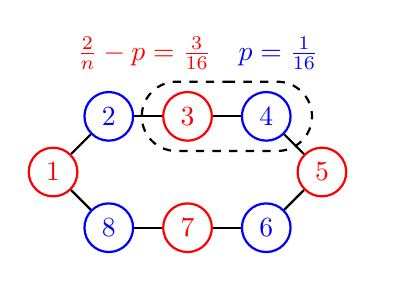
\begin{tikzpicture}[baseline=(current bounding box.north),-,auto,node distance=1cm,
                    thick,main node/.style={circle,draw,font=\sffamily\bfseries}]

  \node[main node,color=red] (1) {$1$};
  \node[main node,color=blue] (2) [above right of=1] {$2$};
  \node[main node,color=red] (3) [right of=2] {$3$};
  \node[main node,color=blue] (4) [right of=3] {$4$};
  \node[main node,color=red] (5) [below right of=4] {$5$};
  \node[main node,color=blue] (6) [below left of=5] {$6$};
  \node[main node,color=red] (7) [left of=6] {$7$};
  \node[main node,color=blue] (8) [left of=7] {$8$};
  

  \path[every node/.style={font=\sffamily}]
  (1) edge (2)
  (2) edge (3)
  (3) edge (4)
  (4) edge (5)
  (5) edge (6)
  (6) edge (7)
  (7) edge (8)
  (8) edge (1);
  
  \node (Box1) [draw,dashed,rounded rectangle,fit=(3) (4)] {};
  
  \node [shift={(-0.4cm,0.8cm)},text width=2cm,color=red] at (3) {$\frac{2}{n}-p=\frac{3}{16}$};
  \node [shift={(0.4cm,0.8cm)},text width=1.5cm,color=blue] at (4) {$p=\frac{1}{16}$};
   
\end{tikzpicture}
\end{center}
\caption{$C_{8}$ with the \textcolor{blue}{blue nodes being ``even'' nodes} started at with probability $\frac{1}{16}$ and the \textcolor{red}{red nodes being ``odd'' nodes} started at with probability $\frac{3}{16}$.}
\end{myfigure}

\begin{lemma}
When $n$ and $m$ are both even, following the ARHP gives the same lower bound as the random Hamiltonian patrol, i.e $V \geq \frac{m}{n}$.
\end{lemma}

\begin{proof}
During any attack interval $I$ which is of even length, then $W(I)$ contains $m'$ ``even'' and $m'$ ``odd'' nodes for a total of $m=2m'$ nodes. Therefore by following the Alternating Random Hamiltonian Patrol, $\pmb{\pi}_{ARHP}$, with probability $p$ at ``even'' nodes and probability $\frac{2}{n}-p$ at ``odd'' nodes. Then

\begin{align*}
&P(\bm{\pi}_{ARHP},[i,I]) \geq \underbrace{\overbrace{p}^{\text{even node}}+\overbrace{\frac{2}{n}-p}^{\text{odd node}}+p+\frac{2}{n}-p+...+p+\frac{2}{n}-p}_{m=2m' \text{ elements}} \\
&=m' p+m'(\frac{2}{n}-p)=\frac{2m'}{n}=\frac{m}{n} \quad \forall i \in N \quad \forall I \subseteq \mathcal{T}
\end{align*}
Hence as it holds for all pure attacks
$$P(\bm{\pi}_{ARHP},\bm{\phi}) \geq \frac{m}{n} \quad \forall \bm{\phi} \in \Phi$$
Hence $V \geq \frac{m}{n}$ .
\end{proof}

If $m$ is odd, say $m=2m'+1$ then in the above we get two possibilities for each node depending on the interval choice either $p+\frac{m-1}{n}$ or $\frac{m+1}{n}-p$. So choosing anything other than $p=\frac{1}{n}$ (which is the Random Hamiltonian Patrol strategy) gives a worse result for the patroller.

While not getting a better lower bound, the ARHP does give some control on how to perform optimally in a Hamiltonian graph. The idea of distributing the probability $\frac{2}{n}$ between two types of nodes can be extended to the idea of distributing the probability $\frac{k}{n}$ between $k$ types of nodes (as seen in Appendix \ref{Appendix:Generalised ARHP}).


We now look at extending the idea of the diametric attack. First we notice that we are not forced to use the graph's diameter, $\bar{d}$, and in fact we can use any distance between two selected nodes, $d$. We replace $\bar{d}$ with $d$ to get a two node distance attack, giving us a bound of $V \leq \max \{\frac{1}{2} ,\frac{m}{2d} \}$. However this cannot be a better bound than using the graph's diameter, so this is not useful.

A useful extension, would be not using two nodes but using multiple points each the same distance apart from each other mutually.

\begin{definition}[Polygonal attack]
A \textit{$d$-polygonal attack} is an attack at a set of nodes $D$ such that $d(i,i')=d \; \forall i,i' \in D$ at the time intervals $I,I+1,...,I+d-1$, for some fixed time interval $I$.
\end{definition}

We can also consider having the points at least the same distance apart, instead of the same distance apart. This construction is considered as it is less restricting on the graphical structure and still provides the same bound.

\begin{definition}[Uneven polygonal attack]
A \textit{$d$-uneven polygonal attack} is an attack at a set of nodes $D$ such that $d(i,i') \geq d \; \forall i,i' \in D$ at the time intervals $I,I+1,...,I+d-1$, for some fixed time interval $I$.
\end{definition}

We need to consider the feasibility of these attacks, due to requiring $d$ potential starting times, we need that $T \geq m-d+1$. The idea behind this attack is very similar to the timed-limited diametric attack, and the proof follows the same logic (expect with more `diametric' nodes each some distance at least $d$ away from all others).

\begin{lemma}
When $T \geq m+d-1$ and a set $D$ as in the $d$- polygonal attack, the bound $V \leq \max \{ \frac{1}{|D|} , \frac{m}{|D|d} \}$ is valid.
\end{lemma}

We conjecture that the uneven-polygonal attack also has the same bound as the polygonal one, as the idea is that any that are strictly greater are just worse for the patroller.

\subsection{Star graph solution}
As a special case of complete bipartite graph we have the star graph, $S_{n}=K_{1,n}$, that is a tree with one internal node (the centre) and $n$ leaf nodes (the external nodes). Hence $V(S_{n})=V(K_{1,n})=\frac{m}{2n}$ for $m<2n$ (by Theorem 15 (1) in \cite{Lin2013}). This is achieved by the patroller forming a patrol which alternates between different  external nodes and the centre, and embedded Hamiltonian patrol from $C_{2n}$, and the attacker attacking at all the external nodes with equal probability for a fixed time interval (or two consecutive time intervals if $m$ is odd).

\subsection{Elongating the star graph}
The line and star graphs provided a good starting point for attempting to solve the problem for a general tree graph. If a more general version of the star graph can be solved, it may provide better bounds on tree graphs. 

The idea is to extend the star graph to a more general graph, which is a mix between the line and the star, by extending the length of the branches (at first just one branch). This may better model a tightly packed region to search and another that is far away, consider the example of a small town and larger city connected by a road. 

\begin{definition}[Elongated Star Graph]
The \textit{Elongated Star Graph}, $S_{n}^{k}$ is made from $S_{n}$, by performing subdivision on one of the edges repeatedly $k$ times, so that one of the external nodes is now $k+1$ away from the centre.
\end{definition}

The labelling will be done as in figure \ref{Figure:Example of elongated labelling}, we note that $*$ nodes are symmetric and so we will be dealing with strategies that treat them as equal (see section 3.1 in \cite{Lin2013}). We will from now assume that $n \geq 3$, as otherwise we are just dealing with the line graph, however we can think of $n=2$ to get the results for the line graph for comparison.


\begin{myfigure}
\begin{center}
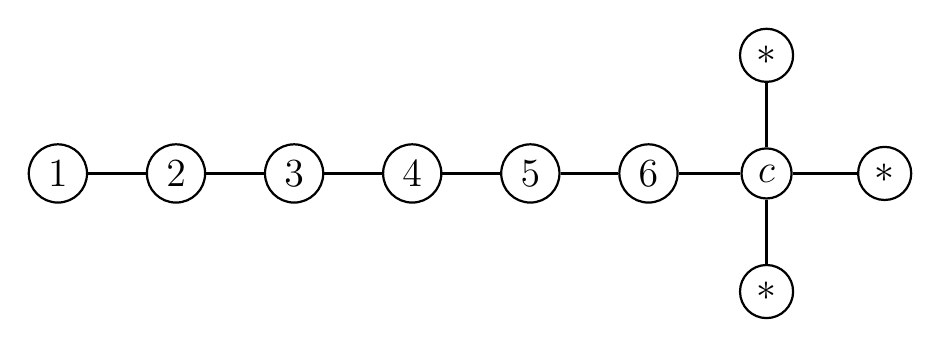
\begin{tikzpicture}[-,auto,node distance=1.5cm,
                    thick,main node/.style={circle,draw,font=\sffamily\Large\bfseries}]

  \node[main node] (1) {$1$};
  \node[main node] (2) [right of=1] {$2$};
  \node[main node] (3) [right of=2] {$3$};
  \node[main node] (4) [right of=3] {$4$};
  \node[main node] (5) [right of=4] {$5$};
  \node[main node] (6) [right of=5]  {$6$};
  \node[main node] (7) [right of=6]  {$c$};
  \node[main node] (8) [right of=7]  {$*$};
  \node[main node] (9) [above of=7]  {$*$};
  \node[main node] (10) [below of=7]  {$*$};
  

  \path[every node/.style={font=\sffamily}]
    (1) edge  (2)
    (2) edge (3)
    (3) edge (4)
    (4) edge (5)
    (5) edge (6)
    (6) edge (7)
    (7) edge (8)
     edge (9)
     edge (10);
\end{tikzpicture}
\end{center}
\caption{Labeling on the graph $S_{4}^5$.}
\label{Figure:Example of elongated labelling}
\end{myfigure}

To start our analysis of this graph, we can look at an expanded graph which can simplify down to our extended star graph. Consider the cyclic graph $C_{(2k+1)+(2n-1)}=C_{2(n+k)}$, we can simplify this graph to $S_{n}^{k}$.


\begin{myfigure}
\begin{center}
\resizebox{\textwidth}{!}{
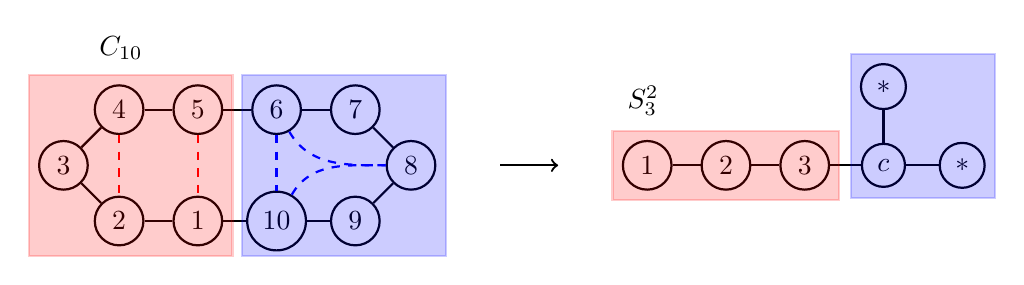
\begin{tikzpicture}[baseline=(current bounding box.north),-,auto,node distance=1cm,
                    thick,main node/.style={circle,draw,font=\sffamily\bfseries}]

  \node[main node] (1) {$3$};
  \node[main node] (2) [above right of=1] {$4$};
  \node[main node] (3) [right of=2] {$5$};
  \node[main node] (4) [right of=3] {$6$};
  \node[main node] (5) [right of=4] {$7$};
  \node[main node] (6) [below right of=5] {$8$};
  \node[main node] (7) [below right of=1] {$2$};
  \node[main node] (8) [right of=7] {$1$};
  \node[main node] (9) [right of=8] {$10$};
  \node[main node] (10) [right of=9] {$9$};
  
  \node (P1) [right of=6] {};
  \node (P2) [right of=P1] {};
  
  \node[main node] (a) [right of=P2] {$1$};
  \node[main node] (b) [right of=a] {$2$};
  \node[main node] (c) [right of=b] {$3$};
  \node[main node] (d) [right of=c] {$c$};
  \node[main node] (e) [right of=d] {$*$};
  \node[main node] (f) [above of=d] {$*$};
  
  \draw[->] (P1) edge (P2);
  

  \path[every node/.style={font=\sffamily}]
    (1) edge  (2)
    edge (7)
    (2) edge (3)
    (3) edge (4)
    (4) edge (5)
    (5) edge (6)
    (6) edge (10)
    (7) edge (8)
    (8) edge (9)
    (9) edge (10)
    (a) edge (b)
    (b) edge (c)
    (c) edge (d)
    (d) edge (e)
    edge (f);
    
     \path[dashed,red,every node/.style={font=\sffamily}]
    (2) edge  (7)
    (3) edge (8);
    
    \path[dashed,blue,every node/.style={font=\sffamily}]
    (4) edge  (9);
    
    \path[dashed,blue,out=-60,in=180,every node/.style={font=\sffamily}]
    (4) edge (6);
    
    \path[dashed,blue,out=60,in=180,every node/.style={font=\sffamily}]
    (9) edge (6);
  
  \node (Box1) [draw,thick,fit=(1) (2) (3) (7) (8),fill,red,opacity=0.2] {};
  \node (Box2) [draw,thick,fit=(4) (5) (6)  (10),fill,blue,opacity=0.2] {};
  
  \node (Box3) [draw,thick,fit=(a) (b) (c),fill,red,opacity=0.2] {}; 
  \node (Box4) [draw,thick,fit=(d) (e) (f),fill,blue,opacity=0.2] {};   
  
\node [left=0.5cm,above=0.5cm,text width=0.5cm] at (2) {$C_{10}$};
\node [left=0.5cm,above=0.5cm,text width=0.5cm] at (a) {$S_{3}^{2}$};   
\end{tikzpicture}
}
\end{center}
\caption{$C_{10}$ can be simplified to $S_{3}^{2}$ by node identifying.}
\end{myfigure}


\begin{definition}[Random Oscillation]
The simplification map from $C_{2(n+k)}$ to $S_{n}^{k}$ is a mapping form nodes $i$ and $2k+2-i$ to node $i$ for $i=1,...,k$ and $2k,2k+2,...,2k+2n-2$ to node $c$ and $2k+2j-1$ to node $*$ for $j=1,...,n-1$.

The \textit{oscillation} on $S_{n}^{k}$ is any embedded Hamiltonian patrol on $C_{2(n+k)}$ under the simplification above.

The \textit{random oscillation} on $S_{n}^{k}$ is the embedded random Hamiltonian patrol on $C_{2(n+k)}$ under the simplification above.
\end{definition}

\begin{lemma}
For $m \leq 2(n+k)$ following the Random Oscillation,
$$V(S_{n}^{k}) \geq \frac{m}{2(n+k)}$$
and if $m > 2(n+k)$ then $V(S_{n}^{k})=1$, achieved by any Oscillation.
\end{lemma}

The proof follows immediately from the simplification bound (Lemma 1 (4) in \cite{Alpern2011}) and the Hamiltonian solution (Theorem 13 (1) in \cite{Alpern2011}) i.e.

\begin{align*}
V(S_{n}^{k}) \geq V(C_{2(n+k)})=\frac{m}{2(n+k)}
\end{align*}

Hence we have the solution in $m > 2(n+k)$ , so we can now restrict ourselves to $m \leq 2(n+k)$.


\begin{note}
We have the solution for $m=2(n+k)$, but to be consistent with the regions in the line graph, we will pull this into the next region.
\end{note}

We could now consider applying the time-limited diametric attack to get bounds on the problem, $\bar{d}=n-1$ gives the bound $V \leq \max \{\frac{1}{2} , \frac{m}{2(n-1)}  \}$, however this bound is not tight with our random oscillation bound, this is because we are not utilising all $*$ type nodes.

Instead of using just one $*$ node (which by symmetry will never yield optimal) we must utilise all the $*$ nodes equally, we can use weights on the distance from the centre. However when using these weights we must spread out  the attack at each position in time, to ensure each potential attack in space and time has an equal weight.

Similiar to the proof of the bipartite graph bounds(Theorem 15 (1) in \cite{Alpern2011}), a timing issue arises when $m$ is odd, however using two fixed time intervals fixes this problem. This holds even when $m$ is even, hence to avoid the problem we will use a baseline spread of two consecutive time periods and then spread out from these according to the weight.

\begin{definition}[Time-delayed attack]
Let the \textit{time-delayed attack}, be the attack that attacks at the extended node labeled $1$ with probability $\frac{k+1}{n+k}$ and a particular normal node labeled $*$ with probability $\frac{1}{n+k}$.

If node $1$ is chosen for the attack, choose time intervals, $I,I+1,...,I+2k+1$, each with equal probability for some fixed time interval, $I$ (i.e starting attacks at $\tau, \tau+1,...,\tau+2k+1$ equiprobably). If a $*$ node is chosen for the attack, choose time intervals, $I+k,I+k+1$, each with equal probability(i.e starting at times $\tau+k,\tau+k+1$ equiprobably).
\end{definition}

A diagram showing how the potential attacks are spaced out in time can be seen in figure \ref{Figure:Time spacing of the time-delayed attack}.

\begin{myfigure}
\begin{center}
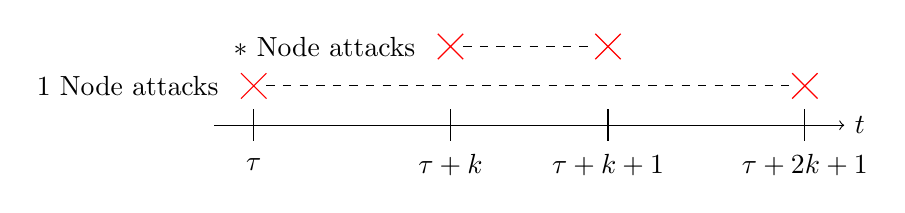
\begin{tikzpicture}
 %Drawing Bottom Axis
 \draw[->] (-4,0) -- (4,0);
 \node (timelabel) [shift={(0.2,0)}] at (4,0) {$t$};
 \draw (-3.5,0.2) -- (-3.5,-0.2);
 \draw (3.5,0.2) -- (3.5,-0.2);
 
 %Drawing Cross and lines 
 \node (labelc1) at (-3.5,-0.5) {$\tau$};
 \node (labelc2) at (3.5,-0.5) {$\tau+2k+1$};
 
 \node[cross=5pt,red] (c1) at (-3.5,0.5) {};
 \node[cross=5pt,red] (c2) at (3.5,0.5) {};
 \draw[dashed] (c1) -- (c2);
 \node (linelabel1) at (-5.1,0.5) {$1$ Node attacks};
 
 
 \draw (-1,0.2) -- (-1,-0.2);
 \draw (1,0.2) -- (1,-0.2);
 
  \node (labelc3) at (-1,-0.5) {$\tau+k$};
 \node (labelc4) at (1,-0.5) {$\tau+k+1$};
 
 \node[cross=5pt,red] (c3) at (-1,1) {};
 \node[cross=5pt,red] (c4) at (1,1) {};
 \draw[dashed] (c3) -- (c4);
 \node (linelabel1) at (-2.6,1) {$*$ Node attacks}; 

\end{tikzpicture}
\end{center}
\caption{Time spacing of the time-delayed attack, for node $1$ and $*$ nodes.}
\label{Figure:Time spacing of the time-delayed attack}
\end{myfigure}

\begin{note}
By making the spread in time proportional to the weight of attacking the node, each potential attack in space and time has the same weight.
\end{note}

\begin{lemma}
When $T \geq m+2k$, the upper bound $V \leq \max \{ \frac{k+1}{n+k} , \frac{m}{2(n+k)}   \}$  is guaranteed by the time-delayed attack.
\end{lemma}

This bound is analogous to the diametric bound, and as long as we are in the range where $m \geq 2(k+1)$ so the lemma gives $V \leq \frac{m}{2(n+k)}$.

\begin{theorem}[Solution in $m \geq 2(k+1)$]
When $T \geq m+2k$, by the attacker using the time-delayed attack and the patroller using a random oscillation patrol, we achieve the value, when $2(k+1) \leq m \leq 2(n+k)$, of
$$V=\frac{m}{2(n+k)}$$
\end{theorem}

Hence we have a solution for 2 regions $m > 2(n+k)$ and $2(k+1) \leq m \leq 2(n+k)$, which we note are analogous to regions $S_{1}$ and $S_{2}$ in the line graph. Hence prompting definitions for our regions

\begin{itemize}
\item $S_{1}' = \{(n,m,k) \, | \, m > 2(n+k) \}$ which have values $V=1$
\item $S_{2}' = \{(n,m,k) \, | \, 2(k+1) \leq m \leq 2(n+k) \}$ which have values $V=\frac{m}{2(n+k)}$
\end{itemize}

An example of these regions and the elongated star graph's value can be seen in \ref{Figure:Elongated star graph region 1 and 2 value}.

\begin{myfigure}
\begin{center}
% Created by tikzDevice version 0.10.1 on 2018-06-27 15:22:20
% !TEX encoding = UTF-8 Unicode
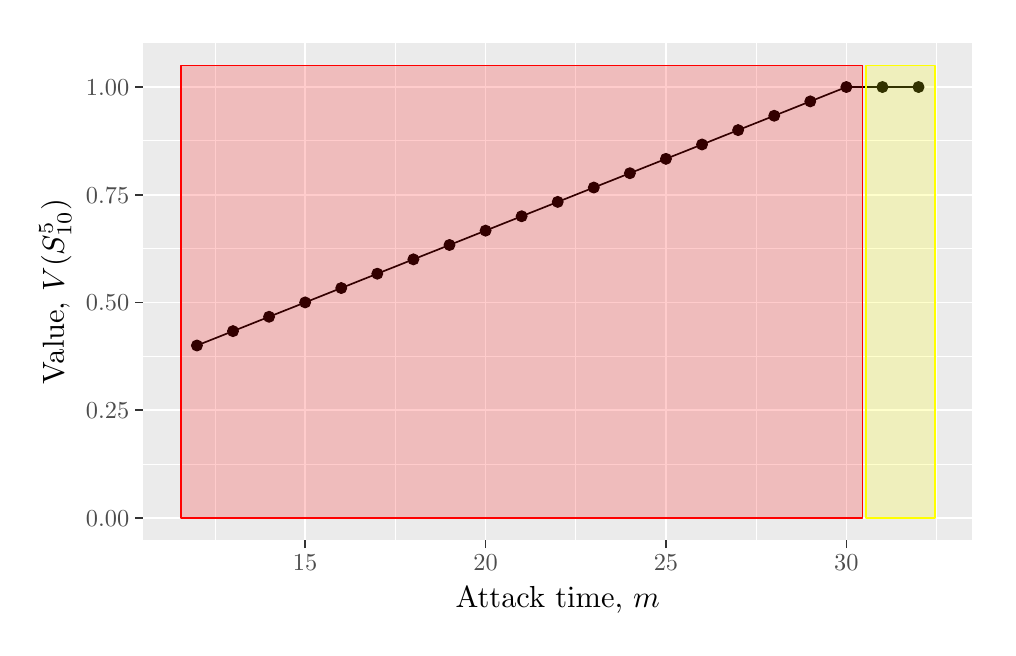
\begin{tikzpicture}[x=1pt,y=1pt]
\definecolor{fillColor}{RGB}{255,255,255}
\path[use as bounding box,fill=fillColor,fill opacity=0.00] (0,0) rectangle (346.90,216.81);
\begin{scope}
\path[clip] (  0.00,  0.00) rectangle (346.90,216.81);
\definecolor{drawColor}{RGB}{255,255,255}
\definecolor{fillColor}{RGB}{255,255,255}

\path[draw=drawColor,line width= 0.6pt,line join=round,line cap=round,fill=fillColor] (  0.00,  0.00) rectangle (346.90,216.81);
\end{scope}
\begin{scope}
\path[clip] ( 41.67, 31.53) rectangle (341.40,211.31);
\definecolor{fillColor}{gray}{0.92}

\path[fill=fillColor] ( 41.67, 31.53) rectangle (341.40,211.31);
\definecolor{drawColor}{RGB}{255,255,255}

\path[draw=drawColor,line width= 0.3pt,line join=round] ( 41.67, 59.16) --
	(341.40, 59.16);

\path[draw=drawColor,line width= 0.3pt,line join=round] ( 41.67, 98.07) --
	(341.40, 98.07);

\path[draw=drawColor,line width= 0.3pt,line join=round] ( 41.67,136.99) --
	(341.40,136.99);

\path[draw=drawColor,line width= 0.3pt,line join=round] ( 41.67,175.90) --
	(341.40,175.90);

\path[draw=drawColor,line width= 0.3pt,line join=round] ( 67.68, 31.53) --
	( 67.68,211.31);

\path[draw=drawColor,line width= 0.3pt,line join=round] (132.86, 31.53) --
	(132.86,211.31);

\path[draw=drawColor,line width= 0.3pt,line join=round] (198.05, 31.53) --
	(198.05,211.31);

\path[draw=drawColor,line width= 0.3pt,line join=round] (263.24, 31.53) --
	(263.24,211.31);

\path[draw=drawColor,line width= 0.3pt,line join=round] (328.42, 31.53) --
	(328.42,211.31);

\path[draw=drawColor,line width= 0.6pt,line join=round] ( 41.67, 39.70) --
	(341.40, 39.70);

\path[draw=drawColor,line width= 0.6pt,line join=round] ( 41.67, 78.62) --
	(341.40, 78.62);

\path[draw=drawColor,line width= 0.6pt,line join=round] ( 41.67,117.53) --
	(341.40,117.53);

\path[draw=drawColor,line width= 0.6pt,line join=round] ( 41.67,156.44) --
	(341.40,156.44);

\path[draw=drawColor,line width= 0.6pt,line join=round] ( 41.67,195.36) --
	(341.40,195.36);

\path[draw=drawColor,line width= 0.6pt,line join=round] (100.27, 31.53) --
	(100.27,211.31);

\path[draw=drawColor,line width= 0.6pt,line join=round] (165.46, 31.53) --
	(165.46,211.31);

\path[draw=drawColor,line width= 0.6pt,line join=round] (230.64, 31.53) --
	(230.64,211.31);

\path[draw=drawColor,line width= 0.6pt,line join=round] (295.83, 31.53) --
	(295.83,211.31);
\definecolor{drawColor}{RGB}{0,0,0}
\definecolor{fillColor}{RGB}{0,0,0}

\path[draw=drawColor,line width= 0.4pt,line join=round,line cap=round,fill=fillColor] (308.87,195.36) circle (  1.96);

\path[draw=drawColor,line width= 0.4pt,line join=round,line cap=round,fill=fillColor] (321.91,195.36) circle (  1.96);

\path[draw=drawColor,line width= 0.4pt,line join=round,line cap=round,fill=fillColor] ( 61.16,101.96) circle (  1.96);

\path[draw=drawColor,line width= 0.4pt,line join=round,line cap=round,fill=fillColor] ( 74.19,107.15) circle (  1.96);

\path[draw=drawColor,line width= 0.4pt,line join=round,line cap=round,fill=fillColor] ( 87.23,112.34) circle (  1.96);

\path[draw=drawColor,line width= 0.4pt,line join=round,line cap=round,fill=fillColor] (100.27,117.53) circle (  1.96);

\path[draw=drawColor,line width= 0.4pt,line join=round,line cap=round,fill=fillColor] (113.31,122.72) circle (  1.96);

\path[draw=drawColor,line width= 0.4pt,line join=round,line cap=round,fill=fillColor] (126.34,127.91) circle (  1.96);

\path[draw=drawColor,line width= 0.4pt,line join=round,line cap=round,fill=fillColor] (139.38,133.09) circle (  1.96);

\path[draw=drawColor,line width= 0.4pt,line join=round,line cap=round,fill=fillColor] (152.42,138.28) circle (  1.96);

\path[draw=drawColor,line width= 0.4pt,line join=round,line cap=round,fill=fillColor] (165.46,143.47) circle (  1.96);

\path[draw=drawColor,line width= 0.4pt,line join=round,line cap=round,fill=fillColor] (178.49,148.66) circle (  1.96);

\path[draw=drawColor,line width= 0.4pt,line join=round,line cap=round,fill=fillColor] (191.53,153.85) circle (  1.96);

\path[draw=drawColor,line width= 0.4pt,line join=round,line cap=round,fill=fillColor] (204.57,159.04) circle (  1.96);

\path[draw=drawColor,line width= 0.4pt,line join=round,line cap=round,fill=fillColor] (217.61,164.22) circle (  1.96);

\path[draw=drawColor,line width= 0.4pt,line join=round,line cap=round,fill=fillColor] (230.64,169.41) circle (  1.96);

\path[draw=drawColor,line width= 0.4pt,line join=round,line cap=round,fill=fillColor] (243.68,174.60) circle (  1.96);

\path[draw=drawColor,line width= 0.4pt,line join=round,line cap=round,fill=fillColor] (256.72,179.79) circle (  1.96);

\path[draw=drawColor,line width= 0.4pt,line join=round,line cap=round,fill=fillColor] (269.76,184.98) circle (  1.96);

\path[draw=drawColor,line width= 0.4pt,line join=round,line cap=round,fill=fillColor] (282.79,190.17) circle (  1.96);

\path[draw=drawColor,line width= 0.4pt,line join=round,line cap=round,fill=fillColor] (295.83,195.36) circle (  1.96);

\path[draw=drawColor,line width= 0.6pt,line join=round] ( 61.16,101.96) --
	( 74.19,107.15) --
	( 87.23,112.34) --
	(100.27,117.53) --
	(113.31,122.72) --
	(126.34,127.91) --
	(139.38,133.09) --
	(152.42,138.28) --
	(165.46,143.47) --
	(178.49,148.66) --
	(191.53,153.85) --
	(204.57,159.04) --
	(217.61,164.22) --
	(230.64,169.41) --
	(243.68,174.60) --
	(256.72,179.79) --
	(269.76,184.98) --
	(282.79,190.17) --
	(295.83,195.36) --
	(308.87,195.36) --
	(321.91,195.36);
\definecolor{drawColor}{RGB}{255,255,0}
\definecolor{fillColor}{RGB}{255,255,0}

\path[draw=drawColor,line width= 0.6pt,line join=round,fill=fillColor,fill opacity=0.20] (303.00, 39.70) rectangle (327.77,203.14);
\definecolor{drawColor}{RGB}{255,0,0}
\definecolor{fillColor}{RGB}{255,0,0}

\path[draw=drawColor,line width= 0.6pt,line join=round,fill=fillColor,fill opacity=0.20] ( 55.29, 39.70) rectangle (301.70,203.14);
\end{scope}
\begin{scope}
\path[clip] (  0.00,  0.00) rectangle (346.90,216.81);
\definecolor{drawColor}{gray}{0.30}

\node[text=drawColor,anchor=base east,inner sep=0pt, outer sep=0pt, scale=  0.88] at ( 36.72, 36.67) {0.00};

\node[text=drawColor,anchor=base east,inner sep=0pt, outer sep=0pt, scale=  0.88] at ( 36.72, 75.59) {0.25};

\node[text=drawColor,anchor=base east,inner sep=0pt, outer sep=0pt, scale=  0.88] at ( 36.72,114.50) {0.50};

\node[text=drawColor,anchor=base east,inner sep=0pt, outer sep=0pt, scale=  0.88] at ( 36.72,153.41) {0.75};

\node[text=drawColor,anchor=base east,inner sep=0pt, outer sep=0pt, scale=  0.88] at ( 36.72,192.33) {1.00};
\end{scope}
\begin{scope}
\path[clip] (  0.00,  0.00) rectangle (346.90,216.81);
\definecolor{drawColor}{gray}{0.20}

\path[draw=drawColor,line width= 0.6pt,line join=round] ( 38.92, 39.70) --
	( 41.67, 39.70);

\path[draw=drawColor,line width= 0.6pt,line join=round] ( 38.92, 78.62) --
	( 41.67, 78.62);

\path[draw=drawColor,line width= 0.6pt,line join=round] ( 38.92,117.53) --
	( 41.67,117.53);

\path[draw=drawColor,line width= 0.6pt,line join=round] ( 38.92,156.44) --
	( 41.67,156.44);

\path[draw=drawColor,line width= 0.6pt,line join=round] ( 38.92,195.36) --
	( 41.67,195.36);
\end{scope}
\begin{scope}
\path[clip] (  0.00,  0.00) rectangle (346.90,216.81);
\definecolor{drawColor}{gray}{0.20}

\path[draw=drawColor,line width= 0.6pt,line join=round] (100.27, 28.78) --
	(100.27, 31.53);

\path[draw=drawColor,line width= 0.6pt,line join=round] (165.46, 28.78) --
	(165.46, 31.53);

\path[draw=drawColor,line width= 0.6pt,line join=round] (230.64, 28.78) --
	(230.64, 31.53);

\path[draw=drawColor,line width= 0.6pt,line join=round] (295.83, 28.78) --
	(295.83, 31.53);
\end{scope}
\begin{scope}
\path[clip] (  0.00,  0.00) rectangle (346.90,216.81);
\definecolor{drawColor}{gray}{0.30}

\node[text=drawColor,anchor=base,inner sep=0pt, outer sep=0pt, scale=  0.88] at (100.27, 20.52) {15};

\node[text=drawColor,anchor=base,inner sep=0pt, outer sep=0pt, scale=  0.88] at (165.46, 20.52) {20};

\node[text=drawColor,anchor=base,inner sep=0pt, outer sep=0pt, scale=  0.88] at (230.64, 20.52) {25};

\node[text=drawColor,anchor=base,inner sep=0pt, outer sep=0pt, scale=  0.88] at (295.83, 20.52) {30};
\end{scope}
\begin{scope}
\path[clip] (  0.00,  0.00) rectangle (346.90,216.81);
\definecolor{drawColor}{RGB}{0,0,0}

\node[text=drawColor,anchor=base,inner sep=0pt, outer sep=0pt, scale=  1.10] at (191.53,  7.44) {Attack time, $m$};
\end{scope}
\begin{scope}
\path[clip] (  0.00,  0.00) rectangle (346.90,216.81);
\definecolor{drawColor}{RGB}{0,0,0}

\node[text=drawColor,rotate= 90.00,anchor=base,inner sep=0pt, outer sep=0pt, scale=  1.10] at ( 13.08,121.42) {Value, $V(S_{ 10 }^{ 5 })$};
\end{scope}
\end{tikzpicture}

\end{center}
\caption{Value of the elongated star graph, $S_{10}^{5}$}
\label{Figure:Elongated star graph region 1 and 2 value}
\end{myfigure}

We then seek solutions in the region $m < 2(k+1)$, however in this region we are below the random oscillation bound for the patroller and we can suggest some improvement (as in $S_{5}$ in the line graph) from the embedded Hamiltonian bound with. To see the issue and why the random oscillation can be improved we will look at the probability of interception under this patrol strategy.

If the patroller is performing a random oscillation, then for a pure attack at node $i$ the probability of capture is given by (derivation in appendix \ref{Appendix:Reason for probability of interception}),
\begin{equation}
\label{eq:Prob of Interception}
w(i)= \left\{\begin{array}{l}
 \frac{\min(m+2(i-1),2m)}{2(n+k)} \text{  , for } i \leq \frac{n+k}{2} +1, \\
 \frac{\min(m+2(n+k+1-i),2m)}{2(n+k)} \text{  , for } i > \frac{n+k}{2} +1, \\
 \frac{\min(m+2(n-1),nm)}{2(n+k)} \text{  , for } i=c, \\
 \frac{m}{2(n+k)} \text{  , for } i=*. 
\end{array} \right.
\end{equation}
We will call $w(i)$ the probability of \textit{interception} at node $i$.

\begin{myfigure}
\begin{center}
% Created by tikzDevice version 0.10.1 on 2018-06-27 15:02:47
% !TEX encoding = UTF-8 Unicode
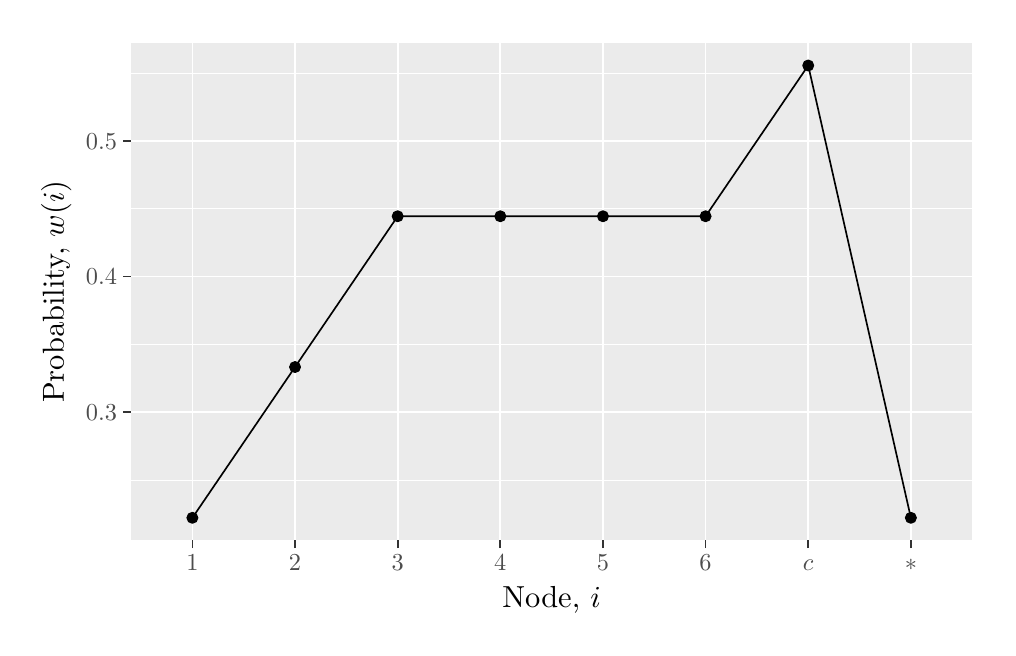
\begin{tikzpicture}[x=1pt,y=1pt]
\definecolor{fillColor}{RGB}{255,255,255}
\path[use as bounding box,fill=fillColor,fill opacity=0.00] (0,0) rectangle (346.90,216.81);
\begin{scope}
\path[clip] (  0.00,  0.00) rectangle (346.90,216.81);
\definecolor{drawColor}{RGB}{255,255,255}
\definecolor{fillColor}{RGB}{255,255,255}

\path[draw=drawColor,line width= 0.6pt,line join=round,line cap=round,fill=fillColor] (  0.00,  0.00) rectangle (346.90,216.81);
\end{scope}
\begin{scope}
\path[clip] ( 37.27, 31.53) rectangle (341.40,211.31);
\definecolor{fillColor}{gray}{0.92}

\path[fill=fillColor] ( 37.27, 31.53) rectangle (341.40,211.31);
\definecolor{drawColor}{RGB}{255,255,255}

\path[draw=drawColor,line width= 0.3pt,line join=round] ( 37.27, 53.32) --
	(341.40, 53.32);

\path[draw=drawColor,line width= 0.3pt,line join=round] ( 37.27,102.35) --
	(341.40,102.35);

\path[draw=drawColor,line width= 0.3pt,line join=round] ( 37.27,151.38) --
	(341.40,151.38);

\path[draw=drawColor,line width= 0.3pt,line join=round] ( 37.27,200.41) --
	(341.40,200.41);

\path[draw=drawColor,line width= 0.6pt,line join=round] ( 37.27, 77.84) --
	(341.40, 77.84);

\path[draw=drawColor,line width= 0.6pt,line join=round] ( 37.27,126.87) --
	(341.40,126.87);

\path[draw=drawColor,line width= 0.6pt,line join=round] ( 37.27,175.90) --
	(341.40,175.90);

\path[draw=drawColor,line width= 0.6pt,line join=round] ( 59.52, 31.53) --
	( 59.52,211.31);

\path[draw=drawColor,line width= 0.6pt,line join=round] ( 96.61, 31.53) --
	( 96.61,211.31);

\path[draw=drawColor,line width= 0.6pt,line join=round] (133.70, 31.53) --
	(133.70,211.31);

\path[draw=drawColor,line width= 0.6pt,line join=round] (170.79, 31.53) --
	(170.79,211.31);

\path[draw=drawColor,line width= 0.6pt,line join=round] (207.88, 31.53) --
	(207.88,211.31);

\path[draw=drawColor,line width= 0.6pt,line join=round] (244.96, 31.53) --
	(244.96,211.31);

\path[draw=drawColor,line width= 0.6pt,line join=round] (282.05, 31.53) --
	(282.05,211.31);

\path[draw=drawColor,line width= 0.6pt,line join=round] (319.14, 31.53) --
	(319.14,211.31);
\definecolor{drawColor}{RGB}{0,0,0}
\definecolor{fillColor}{RGB}{0,0,0}

\path[draw=drawColor,line width= 0.4pt,line join=round,line cap=round,fill=fillColor] ( 59.52, 39.70) circle (  1.96);

\path[draw=drawColor,line width= 0.4pt,line join=round,line cap=round,fill=fillColor] ( 96.61, 94.18) circle (  1.96);

\path[draw=drawColor,line width= 0.4pt,line join=round,line cap=round,fill=fillColor] (133.70,148.66) circle (  1.96);

\path[draw=drawColor,line width= 0.4pt,line join=round,line cap=round,fill=fillColor] (170.79,148.66) circle (  1.96);

\path[draw=drawColor,line width= 0.4pt,line join=round,line cap=round,fill=fillColor] (207.88,148.66) circle (  1.96);

\path[draw=drawColor,line width= 0.4pt,line join=round,line cap=round,fill=fillColor] (244.96,148.66) circle (  1.96);

\path[draw=drawColor,line width= 0.4pt,line join=round,line cap=round,fill=fillColor] (282.05,203.14) circle (  1.96);

\path[draw=drawColor,line width= 0.4pt,line join=round,line cap=round,fill=fillColor] (319.14, 39.70) circle (  1.96);

\path[draw=drawColor,line width= 0.6pt,line join=round] ( 59.52, 39.70) --
	( 96.61, 94.18) --
	(133.70,148.66) --
	(170.79,148.66) --
	(207.88,148.66) --
	(244.96,148.66) --
	(282.05,203.14) --
	(319.14, 39.70);
\end{scope}
\begin{scope}
\path[clip] (  0.00,  0.00) rectangle (346.90,216.81);
\definecolor{drawColor}{gray}{0.30}

\node[text=drawColor,anchor=base east,inner sep=0pt, outer sep=0pt, scale=  0.88] at ( 32.32, 74.81) {0.3};

\node[text=drawColor,anchor=base east,inner sep=0pt, outer sep=0pt, scale=  0.88] at ( 32.32,123.84) {0.4};

\node[text=drawColor,anchor=base east,inner sep=0pt, outer sep=0pt, scale=  0.88] at ( 32.32,172.87) {0.5};
\end{scope}
\begin{scope}
\path[clip] (  0.00,  0.00) rectangle (346.90,216.81);
\definecolor{drawColor}{gray}{0.20}

\path[draw=drawColor,line width= 0.6pt,line join=round] ( 34.52, 77.84) --
	( 37.27, 77.84);

\path[draw=drawColor,line width= 0.6pt,line join=round] ( 34.52,126.87) --
	( 37.27,126.87);

\path[draw=drawColor,line width= 0.6pt,line join=round] ( 34.52,175.90) --
	( 37.27,175.90);
\end{scope}
\begin{scope}
\path[clip] (  0.00,  0.00) rectangle (346.90,216.81);
\definecolor{drawColor}{gray}{0.20}

\path[draw=drawColor,line width= 0.6pt,line join=round] ( 59.52, 28.78) --
	( 59.52, 31.53);

\path[draw=drawColor,line width= 0.6pt,line join=round] ( 96.61, 28.78) --
	( 96.61, 31.53);

\path[draw=drawColor,line width= 0.6pt,line join=round] (133.70, 28.78) --
	(133.70, 31.53);

\path[draw=drawColor,line width= 0.6pt,line join=round] (170.79, 28.78) --
	(170.79, 31.53);

\path[draw=drawColor,line width= 0.6pt,line join=round] (207.88, 28.78) --
	(207.88, 31.53);

\path[draw=drawColor,line width= 0.6pt,line join=round] (244.96, 28.78) --
	(244.96, 31.53);

\path[draw=drawColor,line width= 0.6pt,line join=round] (282.05, 28.78) --
	(282.05, 31.53);

\path[draw=drawColor,line width= 0.6pt,line join=round] (319.14, 28.78) --
	(319.14, 31.53);
\end{scope}
\begin{scope}
\path[clip] (  0.00,  0.00) rectangle (346.90,216.81);
\definecolor{drawColor}{gray}{0.30}

\node[text=drawColor,anchor=base,inner sep=0pt, outer sep=0pt, scale=  0.88] at ( 59.52, 20.52) {$1$};

\node[text=drawColor,anchor=base,inner sep=0pt, outer sep=0pt, scale=  0.88] at ( 96.61, 20.52) {$2$};

\node[text=drawColor,anchor=base,inner sep=0pt, outer sep=0pt, scale=  0.88] at (133.70, 20.52) {$3$};

\node[text=drawColor,anchor=base,inner sep=0pt, outer sep=0pt, scale=  0.88] at (170.79, 20.52) {$4$};

\node[text=drawColor,anchor=base,inner sep=0pt, outer sep=0pt, scale=  0.88] at (207.88, 20.52) {$5$};

\node[text=drawColor,anchor=base,inner sep=0pt, outer sep=0pt, scale=  0.88] at (244.96, 20.52) {$6$};

\node[text=drawColor,anchor=base,inner sep=0pt, outer sep=0pt, scale=  0.88] at (282.05, 20.52) {$c$};

\node[text=drawColor,anchor=base,inner sep=0pt, outer sep=0pt, scale=  0.88] at (319.14, 20.52) {$*$};
\end{scope}
\begin{scope}
\path[clip] (  0.00,  0.00) rectangle (346.90,216.81);
\definecolor{drawColor}{RGB}{0,0,0}

\node[text=drawColor,anchor=base,inner sep=0pt, outer sep=0pt, scale=  1.10] at (189.33,  7.44) {Node, $i$};
\end{scope}
\begin{scope}
\path[clip] (  0.00,  0.00) rectangle (346.90,216.81);
\definecolor{drawColor}{RGB}{0,0,0}

\node[text=drawColor,rotate= 90.00,anchor=base,inner sep=0pt, outer sep=0pt, scale=  1.10] at ( 13.08,121.42) {Probability, $w(i)$};
\end{scope}
\end{tikzpicture}

\end{center}
\caption{Interception probabilities of $S^5_{4}$ when $m=4$.}
\label{Figure:Base interception probabilities}
\end{myfigure}

Looking at the function (or the figure \ref{Figure:Base interception probabilities}) it is clear that the issues are towards the end of the graph. This is because the next return under the random oscillation does not provide adequate coverage, hence we may wish to improve these end points of the graph. To do so we introduce the concepts of cycles which are played to guarantee capture of all attacks at all nodes within their cycle(\textit{covering}).

\begin{definition}[End-covering cycle]
Define a cycle of length $m$ (if even) or $m-1$ (if odd) to be \textit{end-covering} if one of the points along the cycle is a leaf node. Define the \textit{half-length} of such cycles to be $\hat{m}=\floor{\frac{m}{2}}$.
\end{definition}

In \cite{Papadaki2016} the authors improved the line graph's end nodes, which have poor interception probabilities, by introducing a end-covering cycle at each end. We shall do the same, though now more consideration needs to be taken on how to place these end-covering cycles. 

We first classify nodes into types, we partition the node set, $N=L \cup M \cup R \cup S$, where
\begin{itemize}
\item Left nodes, $L=\left\{ i \, | \, i \leq \floor{\frac{m}{2}}+1 , i \leq k+1 \right\}$, 
\item Middle nodes, $M=\left\{ i \, | \, \floor{\frac{m}{2}}+2 \leq i \leq n+k-\floor{\frac{m}{2}} , i \leq k+1 \right\}$,
\item Right nodes, $R=\left\{ i \, | \, i \geq n+k+1-\floor{\frac{m}{2}} , i \leq k+1 \right\}$,
\item Star node, $S=\{ c,* \}$.
\end{itemize}

\begin{note}
The set $R$ is empty if $\hat{m} \leq n-1$. The set $M$ is empty if $\hat{m} \geq k-1$ or $\hat{m} \geq n+k-2$.
\end{note}

Then $ V \geq w_{\min} \equiv w_{\min}^{N}=\min \left\{ w_{\min}^{L},w_{\min}^{M},w_{\min}^{R},w_{\min}^{S} \right\}$ , where $w_{\min}^{X}=\min\limits_{i \in X} w(i)$. We aim to use end-ensuring cycles to improve $w_{\min}$, which means improving the worst node sets, and hence improving the random oscillation bound.


Now from equation \ref{eq:Prob of Interception} we note some properties for each node set.
\begin{itemize}
\item $w_{min}^{L}=w(1)$, as for $i \in L$ we have that $w(i)$ is increasing in $i$.
\item $w_{min}^{M}=w(\hat{m}+2)=\frac{2m}{2(n+k)}$ , as for $i \in M $ we have that $w(i)=\frac{2m}{2(n+k)}$ $\forall i \in M$.
\item $w_{min}^{R}=w(k+1)$, as for $i \in R$ we have that $w(i)$ is decreasing in $i$.
\item $w_{min}^{S}=w(*)$, as $w(c) > w(*)$.
\end{itemize}

So as long as the improvement made on $L$ and $M$ is non-decreasing then only the nodes $1$ and $\hat{m}+2$ need be considered. Similarly if in $R$, the improvement is non-increasing then we only need to consider the node $k+1$.Finally if in $S$, the improvement improves node $c$ as good as $*$ then we only need to consider $*$. We shall only consider improving strategies of the type above so only nodes, $1,\hat{m}+2,k+1,*$(if the set is non-empty) need to be considered.

Similarly let $C_{\min}^{X} (\bm{\pi}) = \min\limits_{i \in X} P(\bm{\pi},i)$, where $P(\bm{\pi},i)=\max\limits_{ I \subset \mathcal{T}} P(\bm{\pi},[i,I])$, is the probability of capture under $\bm{\pi}$ and $C_{\min} (\bm{\pi}) \equiv C_{\min}^{N} = \min \left\{ C_{\min}^{L},  C_{\min}^{M},  C_{\min}^{R},  C_{\min}^{S} \right\}$. Then we seek to select $\bm{\pi}$ to get $C_{\min} (\bm{\pi}) > W_{\min} \equiv C_{\min}(\bm{\pi}_{0})$ , where $\bm{\pi}_{0}$ is the random oscillation strategy.

We will use $P$ to be the probability that the random oscillation is played, and $Q=1-P$, to be the probability the improvement is played. We split, $Q$ into $Q=Q_{L}+Q_{M}+Q_{R}+Q_{S}$, where $Q_{X}$ is the amount of probability used to improve the probability of intersection for the set $X$. We use $q_{X}$ to be probability that the minimum of the set is improved by, so $C_{\min}^{X}=PW_{\min}^{X}+q_{X}$.

Multiple choices for possible improvement exist, we first present the most simplest, but naive improvement. The improvement will begin by imagining the $*$ nodes are the ends of $n-1$ lines and improve as in the improvment to the line's hamiltonian bound(section 5 in \cite{Papadaki2016}). Because this approach is naive and is not fully utilising our graphical structure, we will adopt a combinatorial approach to which nodes to improve.

\textbf{A naive improvement}
Let $\bm{\pi}=\bm{\pi}_{N}(Q_{L},Q_{S})$ denote the naive improvement policy. We will play the end-ensuring cycle, $\{1,...,\hat{m}+1,...,1\}$, with probability $Q_{L}$ (a non-decreasing improvement), giving $q_{L}=Q_{L}$. We will play an end-covering cycle for each $*$ node, $\{*,c,....,k+3-\hat{m},....,c,* \}$,(a non-decreasing improvement) with total probability $Q_{S}$, giving $q_{S}=\frac{Q_{S}}{n-1}$.
 
Now we may also have improved some of the nodes in $R$, possibly up to node $k+3-\hat{m} \leq n+k+1-\hat{m}$ (as $n \geq 3$), meaning that all nodes in $R$ are in the end-covering cycle,   $\{*,c,...,k+3-\floor{\frac{m}{2}} \}$ , so the improvement is non-increasing, so $q_{R}=q_{S}$. If $M \neq \emptyset$ nodes in $M$ may be improved, but the node $\hat{m} +2$ will not be improved as  $\hat{m} +2 > \hat{m} +1$ and $\hat{m} +2 < k+3- \hat{m}$ (as $\hat{m} < k-1$ when $M \neq \emptyset$), so the improvement is non-decreasing and $q_{M}=0$.


\begin{examplefigure}
\begin{center}
\resizebox{\textwidth}{!}{
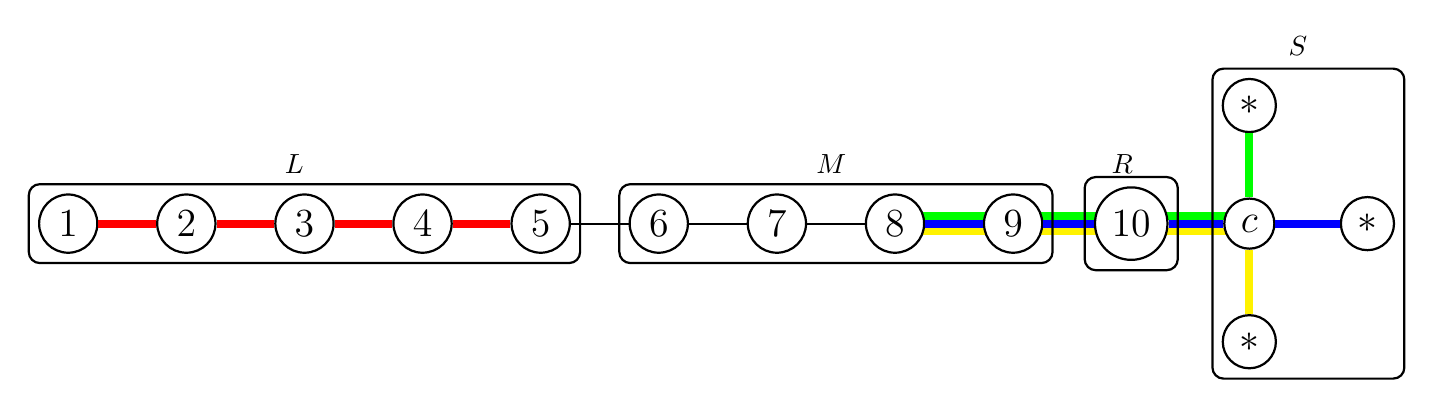
\begin{tikzpicture}[-,auto,node distance=1.5cm,
                    thick,main node/.style={circle,fill=white,draw,font=\sffamily\Large\bfseries}]

  \node[main node] (1) {$1$};
  \node[main node] (2) [right of=1] {$2$};
  \node[main node] (3) [right of=2] {$3$};
  \node[main node] (4) [right of=3] {$4$};
  \node[main node] (5) [right of=4] {$5$};
  \node[main node] (6) [right of=5]  {$6$};
  \node[main node] (7) [right of=6] {$7$};
  \node[main node] (8) [right of=7] {$8$};
  \node[main node] (9) [right of=8] {$9$};
  \node[main node] (10) [right of=9]  {$10$};
  \node[main node] (11) [right of=10]  {$c$};
  \node[main node] (12) [right of=11]  {$*$};
  \node[main node] (13) [above of=11]  {$*$};
  \node[main node] (14) [below of=11]  {$*$};
  

  \path[every node/.style={font=\sffamily}]
    (1) edge  (2)
    (2) edge (3)
    (3) edge (4)
    (4) edge (5)
    (5) edge (6)
    (6) edge (7)
    (7) edge (8)
    (8) edge (9)
    (9) edge (10)
    (10) edge (11)
    (11) edge (12)
    edge (13)
    edge (14);
      
     
   \draw[line width=1mm,color=red] (1) to (2) to (3) to (4) to (5);
   
   \draw [line width=1mm,color=blue] (11) to (12);
   \draw [line width=1mm,color=green] (11) to (13);
   \draw [line width=1mm,color=yellow] (11) to (14);
   \draw [line width=1mm,color=blue] (8) to (9) to (10) to (11);
   
   \node (LBox) [draw,rounded corners, fit= (1) (2) (3) (4) (5)] {};
   \node (MBox) [draw,rounded corners, fit= (6) (7) (8) (9)] {};
   \node (RBox) [draw,rounded corners, fit= (10)] {};
   \node (SBox) [draw,rounded corners, fit= (11) (12) (13) (14)] {};
   
   \node [above=0.5cm,text width=0.5cm] at (LBox) {$L$};
   \node [above=0.5cm,text width=0.5cm] at (MBox) {$M$};
   \node [above=0.5cm,text width=0.5cm] at (RBox) {$R$};
   \node [,above=2cm,text width=0.5cm] at (SBox) {$S$}; 
   
\begin{scope}[on background layer]
   \node[style={circle,,font=\sffamily\Large\bfseries}] (8H) at ($ (8) + (0,0.1) $) { };
   \node[style={circle,,font=\sffamily\Large\bfseries}] (9H) at ($ (9) + (0,0.1) $) { };   
   \node[style={circle,,font=\sffamily\Large\bfseries}] (10H) at ($ (10) + (0,0.1) $) { };
   \node[style={circle,,font=\sffamily\Large\bfseries}] (11H) at ($ (11) + (0,0.1) $) { };
   \draw [line width=1mm,color=green] (8H) to (9H) to (10H) to (11H);
   \node[style={circle,,font=\sffamily\Large\bfseries}] (8L) at ($ (8) + (0,-0.1) $) { };
   \node[style={circle,,font=\sffamily\Large\bfseries}] (9L) at ($ (9) + (0,-0.1) $) { };
   \node[style={circle,,font=\sffamily\Large\bfseries}] (10L) at ($ (10) + (0,-0.1) $) { };
   \node[style={circle,,font=\sffamily\Large\bfseries}] (11L) at ($ (11) + (0,-0.1) $) { };
   \draw [line width=1mm,color=yellow] (8L) to (9L) to (10L) to (11L);
\end{scope}
    
   
\end{tikzpicture}
}
\end{center}
\caption{The Naive Improvement on $S_{4}^{9}$ for $m=9$. The \textcolor{red}{red lines indicating the end-covering cycle $\{1,2,3,4,5,4,3,2,1 \}$} and the other coloured lines indicating the end-ensuring cycles, for each $*$, $\{*,c,10,9,8,9,10,c,* \}$ (as $\hat{m}=4$).}
\end{examplefigure}


Using the Naive Improvement Policy we can achieve an improvement over the random oscillation if $2(n+k) -nm \geq 0$ and get a bound of $V \geq \frac{2m}{2(n+k)+nm}$ (or $V \geq \frac{1}{n}$ if $M=\emptyset,R=\emptyset$), by choosing optimal $Q_{L}$ and $Q_{S}$ (See appendix \ref{Appendix:Naive improvement analysis} for the details).


\begin{myfigure}
\begin{center}
% Created by tikzDevice version 0.10.1 on 2018-06-27 15:02:49
% !TEX encoding = UTF-8 Unicode
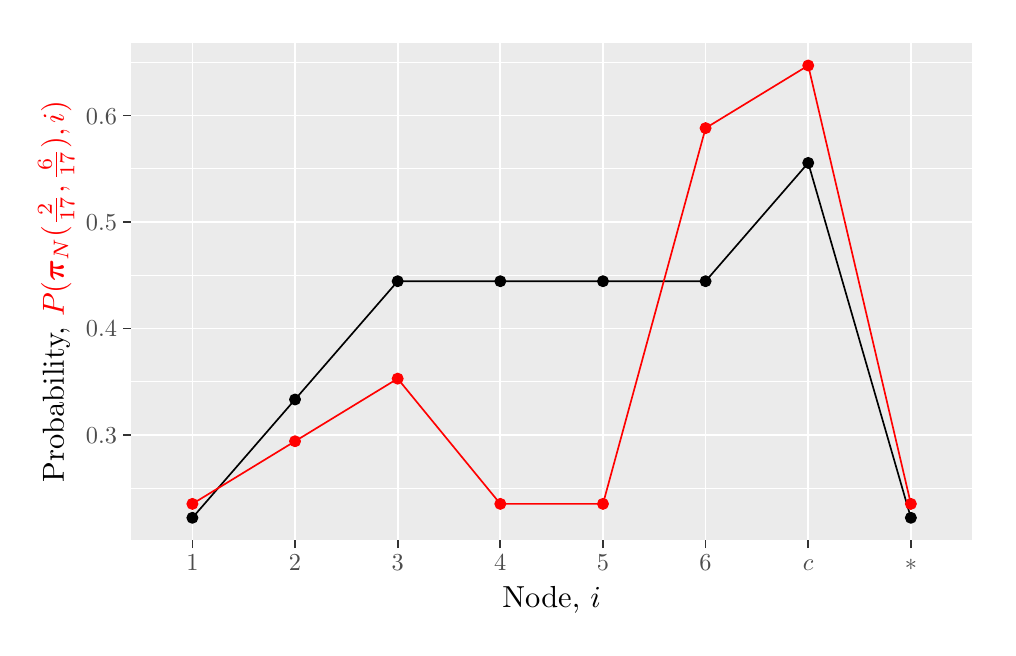
\begin{tikzpicture}[x=1pt,y=1pt]
\definecolor{fillColor}{RGB}{255,255,255}
\path[use as bounding box,fill=fillColor,fill opacity=0.00] (0,0) rectangle (346.90,216.81);
\begin{scope}
\path[clip] (  0.00,  0.00) rectangle (346.90,216.81);
\definecolor{drawColor}{RGB}{255,255,255}
\definecolor{fillColor}{RGB}{255,255,255}

\path[draw=drawColor,line width= 0.6pt,line join=round,line cap=round,fill=fillColor] (  0.00,  0.00) rectangle (346.90,216.81);
\end{scope}
\begin{scope}
\path[clip] ( 37.27, 31.53) rectangle (341.40,211.31);
\definecolor{fillColor}{gray}{0.92}

\path[fill=fillColor] ( 37.27, 31.53) rectangle (341.40,211.31);
\definecolor{drawColor}{RGB}{255,255,255}

\path[draw=drawColor,line width= 0.3pt,line join=round] ( 37.27, 50.39) --
	(341.40, 50.39);

\path[draw=drawColor,line width= 0.3pt,line join=round] ( 37.27, 88.86) --
	(341.40, 88.86);

\path[draw=drawColor,line width= 0.3pt,line join=round] ( 37.27,127.33) --
	(341.40,127.33);

\path[draw=drawColor,line width= 0.3pt,line join=round] ( 37.27,165.80) --
	(341.40,165.80);

\path[draw=drawColor,line width= 0.3pt,line join=round] ( 37.27,204.27) --
	(341.40,204.27);

\path[draw=drawColor,line width= 0.6pt,line join=round] ( 37.27, 69.62) --
	(341.40, 69.62);

\path[draw=drawColor,line width= 0.6pt,line join=round] ( 37.27,108.09) --
	(341.40,108.09);

\path[draw=drawColor,line width= 0.6pt,line join=round] ( 37.27,146.56) --
	(341.40,146.56);

\path[draw=drawColor,line width= 0.6pt,line join=round] ( 37.27,185.03) --
	(341.40,185.03);

\path[draw=drawColor,line width= 0.6pt,line join=round] ( 59.52, 31.53) --
	( 59.52,211.31);

\path[draw=drawColor,line width= 0.6pt,line join=round] ( 96.61, 31.53) --
	( 96.61,211.31);

\path[draw=drawColor,line width= 0.6pt,line join=round] (133.70, 31.53) --
	(133.70,211.31);

\path[draw=drawColor,line width= 0.6pt,line join=round] (170.79, 31.53) --
	(170.79,211.31);

\path[draw=drawColor,line width= 0.6pt,line join=round] (207.88, 31.53) --
	(207.88,211.31);

\path[draw=drawColor,line width= 0.6pt,line join=round] (244.96, 31.53) --
	(244.96,211.31);

\path[draw=drawColor,line width= 0.6pt,line join=round] (282.05, 31.53) --
	(282.05,211.31);

\path[draw=drawColor,line width= 0.6pt,line join=round] (319.14, 31.53) --
	(319.14,211.31);
\definecolor{drawColor}{RGB}{0,0,0}
\definecolor{fillColor}{RGB}{0,0,0}

\path[draw=drawColor,line width= 0.4pt,line join=round,line cap=round,fill=fillColor] ( 59.52, 39.70) circle (  1.96);

\path[draw=drawColor,line width= 0.4pt,line join=round,line cap=round,fill=fillColor] ( 96.61, 82.45) circle (  1.96);

\path[draw=drawColor,line width= 0.4pt,line join=round,line cap=round,fill=fillColor] (133.70,125.19) circle (  1.96);

\path[draw=drawColor,line width= 0.4pt,line join=round,line cap=round,fill=fillColor] (170.79,125.19) circle (  1.96);

\path[draw=drawColor,line width= 0.4pt,line join=round,line cap=round,fill=fillColor] (207.88,125.19) circle (  1.96);

\path[draw=drawColor,line width= 0.4pt,line join=round,line cap=round,fill=fillColor] (244.96,125.19) circle (  1.96);

\path[draw=drawColor,line width= 0.4pt,line join=round,line cap=round,fill=fillColor] (282.05,167.94) circle (  1.96);

\path[draw=drawColor,line width= 0.4pt,line join=round,line cap=round,fill=fillColor] (319.14, 39.70) circle (  1.96);

\path[draw=drawColor,line width= 0.6pt,line join=round] ( 59.52, 39.70) --
	( 96.61, 82.45) --
	(133.70,125.19) --
	(170.79,125.19) --
	(207.88,125.19) --
	(244.96,125.19) --
	(282.05,167.94) --
	(319.14, 39.70);
\definecolor{drawColor}{RGB}{255,0,0}
\definecolor{fillColor}{RGB}{255,0,0}

\path[draw=drawColor,line width= 0.4pt,line join=round,line cap=round,fill=fillColor] ( 59.52, 44.73) circle (  1.96);

\path[draw=drawColor,line width= 0.4pt,line join=round,line cap=round,fill=fillColor] ( 96.61, 67.36) circle (  1.96);

\path[draw=drawColor,line width= 0.4pt,line join=round,line cap=round,fill=fillColor] (133.70, 89.99) circle (  1.96);

\path[draw=drawColor,line width= 0.4pt,line join=round,line cap=round,fill=fillColor] (170.79, 44.73) circle (  1.96);

\path[draw=drawColor,line width= 0.4pt,line join=round,line cap=round,fill=fillColor] (207.88, 44.73) circle (  1.96);

\path[draw=drawColor,line width= 0.4pt,line join=round,line cap=round,fill=fillColor] (244.96,180.51) circle (  1.96);

\path[draw=drawColor,line width= 0.4pt,line join=round,line cap=round,fill=fillColor] (282.05,203.14) circle (  1.96);

\path[draw=drawColor,line width= 0.4pt,line join=round,line cap=round,fill=fillColor] (319.14, 44.73) circle (  1.96);

\path[draw=drawColor,line width= 0.6pt,line join=round] ( 59.52, 44.73) --
	( 96.61, 67.36) --
	(133.70, 89.99) --
	(170.79, 44.73) --
	(207.88, 44.73) --
	(244.96,180.51) --
	(282.05,203.14) --
	(319.14, 44.73);
\end{scope}
\begin{scope}
\path[clip] (  0.00,  0.00) rectangle (346.90,216.81);
\definecolor{drawColor}{gray}{0.30}

\node[text=drawColor,anchor=base east,inner sep=0pt, outer sep=0pt, scale=  0.88] at ( 32.32, 66.59) {0.3};

\node[text=drawColor,anchor=base east,inner sep=0pt, outer sep=0pt, scale=  0.88] at ( 32.32,105.06) {0.4};

\node[text=drawColor,anchor=base east,inner sep=0pt, outer sep=0pt, scale=  0.88] at ( 32.32,143.53) {0.5};

\node[text=drawColor,anchor=base east,inner sep=0pt, outer sep=0pt, scale=  0.88] at ( 32.32,182.00) {0.6};
\end{scope}
\begin{scope}
\path[clip] (  0.00,  0.00) rectangle (346.90,216.81);
\definecolor{drawColor}{gray}{0.20}

\path[draw=drawColor,line width= 0.6pt,line join=round] ( 34.52, 69.62) --
	( 37.27, 69.62);

\path[draw=drawColor,line width= 0.6pt,line join=round] ( 34.52,108.09) --
	( 37.27,108.09);

\path[draw=drawColor,line width= 0.6pt,line join=round] ( 34.52,146.56) --
	( 37.27,146.56);

\path[draw=drawColor,line width= 0.6pt,line join=round] ( 34.52,185.03) --
	( 37.27,185.03);
\end{scope}
\begin{scope}
\path[clip] (  0.00,  0.00) rectangle (346.90,216.81);
\definecolor{drawColor}{gray}{0.20}

\path[draw=drawColor,line width= 0.6pt,line join=round] ( 59.52, 28.78) --
	( 59.52, 31.53);

\path[draw=drawColor,line width= 0.6pt,line join=round] ( 96.61, 28.78) --
	( 96.61, 31.53);

\path[draw=drawColor,line width= 0.6pt,line join=round] (133.70, 28.78) --
	(133.70, 31.53);

\path[draw=drawColor,line width= 0.6pt,line join=round] (170.79, 28.78) --
	(170.79, 31.53);

\path[draw=drawColor,line width= 0.6pt,line join=round] (207.88, 28.78) --
	(207.88, 31.53);

\path[draw=drawColor,line width= 0.6pt,line join=round] (244.96, 28.78) --
	(244.96, 31.53);

\path[draw=drawColor,line width= 0.6pt,line join=round] (282.05, 28.78) --
	(282.05, 31.53);

\path[draw=drawColor,line width= 0.6pt,line join=round] (319.14, 28.78) --
	(319.14, 31.53);
\end{scope}
\begin{scope}
\path[clip] (  0.00,  0.00) rectangle (346.90,216.81);
\definecolor{drawColor}{gray}{0.30}

\node[text=drawColor,anchor=base,inner sep=0pt, outer sep=0pt, scale=  0.88] at ( 59.52, 20.52) {$1$};

\node[text=drawColor,anchor=base,inner sep=0pt, outer sep=0pt, scale=  0.88] at ( 96.61, 20.52) {$2$};

\node[text=drawColor,anchor=base,inner sep=0pt, outer sep=0pt, scale=  0.88] at (133.70, 20.52) {$3$};

\node[text=drawColor,anchor=base,inner sep=0pt, outer sep=0pt, scale=  0.88] at (170.79, 20.52) {$4$};

\node[text=drawColor,anchor=base,inner sep=0pt, outer sep=0pt, scale=  0.88] at (207.88, 20.52) {$5$};

\node[text=drawColor,anchor=base,inner sep=0pt, outer sep=0pt, scale=  0.88] at (244.96, 20.52) {$6$};

\node[text=drawColor,anchor=base,inner sep=0pt, outer sep=0pt, scale=  0.88] at (282.05, 20.52) {$c$};

\node[text=drawColor,anchor=base,inner sep=0pt, outer sep=0pt, scale=  0.88] at (319.14, 20.52) {$*$};
\end{scope}
\begin{scope}
\path[clip] (  0.00,  0.00) rectangle (346.90,216.81);
\definecolor{drawColor}{RGB}{0,0,0}

\node[text=drawColor,anchor=base,inner sep=0pt, outer sep=0pt, scale=  1.10] at (189.33,  7.44) {Node, $i$};
\end{scope}
\begin{scope}
\path[clip] (  0.00,  0.00) rectangle (346.90,216.81);
\definecolor{drawColor}{RGB}{0,0,0}

\node[text=drawColor,rotate= 90.00,anchor=base,inner sep=0pt, outer sep=0pt, scale=  1.10] at ( 13.08,121.42) {Probability, \textcolor{red}{$P(\bm{\pi}_{N}(\frac{2}{17},\frac{6}{17}),i)$}};
\end{scope}
\end{tikzpicture}

\end{center}
\caption{Interception probabilities of $S^5_{4}$ when $m=4$, with the \textcolor{red}{red Probabilities showing the Naive Improvement Policy $\bm{\pi}_{N}\left(\frac{2}{17},\frac{6}{17} \right)$}.}
\end{myfigure}

\textbf{Combinatorial Improvement}

\begin{definition}[Combinatorial Improvement]
Let $\bm{\pi}_{C}(Q_{L},Q_{S})$ denote the combinatorial improvement policy, which improves the sets, $L$ and $S$. An end-covering cycle, $\{ 1,...,\hat{m}+1,...,1 \}$ is played with probability $Q_{L}$, so $q_{L}=Q_{L}$. Also;

\begin{enumerate}
\item[Case i)] If $R \neq \emptyset$ then $\hat{m}=n+r$, for some excess $r$. Then form an end-covering cycle on the nodes $\{ n+k+1-\hat{m},...,k+1,c,*,c,*,...,c,*,c,k+1,...,n+k+1-\hat{m} \}$. This cycle will be played with probability $Q_{S}$ and improves all the nodes in $R$(non-increasing) and $S$($c$ is better than $*$) so $q_{R}=Q_{R}$ and $q_{S}=Q_{S}$.

\item[Case ii)] If $R = \emptyset$ then an end-covering cycle is formed by choosing $\hat{m}$ of the $*$ nodes (now labelled $*_{1},...,*_{\hat{m}}$) each with equal probability and forming a cycle $\{*_{1},c,*_{2},...,c,*_{\hat{m}},c,*_{1} \}$. This construction is performed with probability $Q_{S}$ and nodes in $S$ ($c$ is better than $*$). The actual improvement made for a $*$ node is $$q_{S}=Q_{S} \times \mathbb{P}(\text{A particular } * \text{ node is picked})=Q_{S} \times \frac{\hat{m}}{n-1} $$
\end{enumerate}
\end{definition}

We leave the exact analysis to appendix \ref{Appendix:Combinatorial improvement analysis} but are interested in the bounds: 
\begin{itemize}
\item If $M=\emptyset$,$R=\emptyset$ then $V \geq \frac{\hat{m}}{\hat{m}+n-1}$.
\item If $M \neq \emptyset$,$R=\emptyset$ then $V \geq \frac{2m}{2(n+k)+m(1+\frac{n-1}{\hat{m}})}$.
\item If $M \neq \emptyset$,$R \neq \emptyset$ then $V \geq \frac{2m}{2(n+k+m)}$.
\end{itemize}

\begin{myfigure}
\begin{center}
% Created by tikzDevice version 0.10.1 on 2018-06-27 15:03:08
% !TEX encoding = UTF-8 Unicode
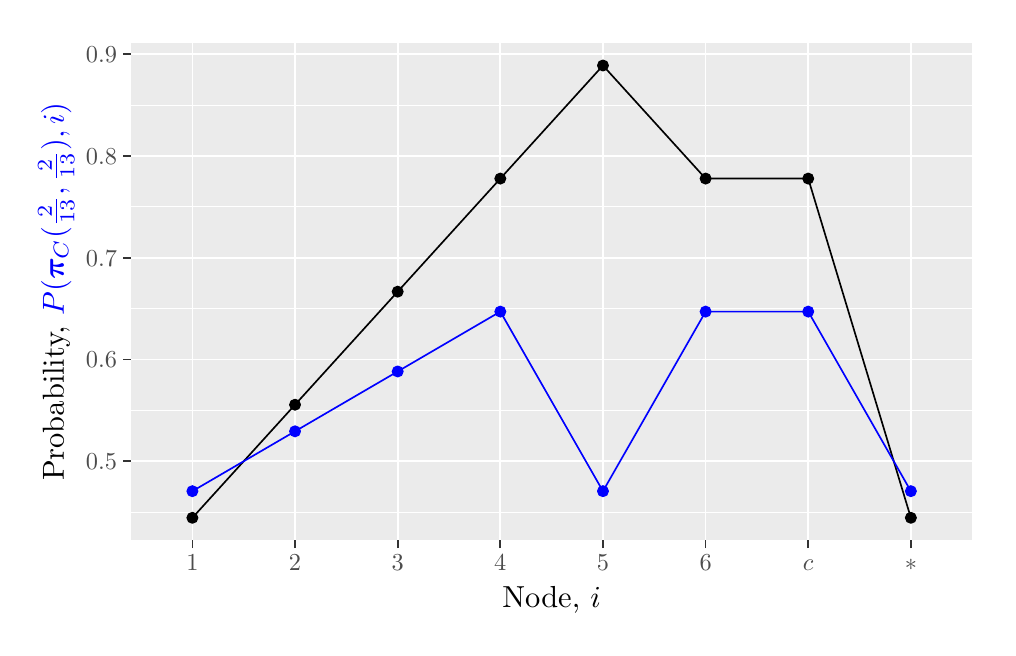
\begin{tikzpicture}[x=1pt,y=1pt]
\definecolor{fillColor}{RGB}{255,255,255}
\path[use as bounding box,fill=fillColor,fill opacity=0.00] (0,0) rectangle (346.90,216.81);
\begin{scope}
\path[clip] (  0.00,  0.00) rectangle (346.90,216.81);
\definecolor{drawColor}{RGB}{255,255,255}
\definecolor{fillColor}{RGB}{255,255,255}

\path[draw=drawColor,line width= 0.6pt,line join=round,line cap=round,fill=fillColor] (  0.00,  0.00) rectangle (346.90,216.81);
\end{scope}
\begin{scope}
\path[clip] ( 37.27, 31.53) rectangle (341.40,211.31);
\definecolor{fillColor}{gray}{0.92}

\path[fill=fillColor] ( 37.27, 31.53) rectangle (341.40,211.31);
\definecolor{drawColor}{RGB}{255,255,255}

\path[draw=drawColor,line width= 0.3pt,line join=round] ( 37.27, 41.75) --
	(341.40, 41.75);

\path[draw=drawColor,line width= 0.3pt,line join=round] ( 37.27, 78.52) --
	(341.40, 78.52);

\path[draw=drawColor,line width= 0.3pt,line join=round] ( 37.27,115.29) --
	(341.40,115.29);

\path[draw=drawColor,line width= 0.3pt,line join=round] ( 37.27,152.06) --
	(341.40,152.06);

\path[draw=drawColor,line width= 0.3pt,line join=round] ( 37.27,188.84) --
	(341.40,188.84);

\path[draw=drawColor,line width= 0.6pt,line join=round] ( 37.27, 60.13) --
	(341.40, 60.13);

\path[draw=drawColor,line width= 0.6pt,line join=round] ( 37.27, 96.90) --
	(341.40, 96.90);

\path[draw=drawColor,line width= 0.6pt,line join=round] ( 37.27,133.68) --
	(341.40,133.68);

\path[draw=drawColor,line width= 0.6pt,line join=round] ( 37.27,170.45) --
	(341.40,170.45);

\path[draw=drawColor,line width= 0.6pt,line join=round] ( 37.27,207.22) --
	(341.40,207.22);

\path[draw=drawColor,line width= 0.6pt,line join=round] ( 59.52, 31.53) --
	( 59.52,211.31);

\path[draw=drawColor,line width= 0.6pt,line join=round] ( 96.61, 31.53) --
	( 96.61,211.31);

\path[draw=drawColor,line width= 0.6pt,line join=round] (133.70, 31.53) --
	(133.70,211.31);

\path[draw=drawColor,line width= 0.6pt,line join=round] (170.79, 31.53) --
	(170.79,211.31);

\path[draw=drawColor,line width= 0.6pt,line join=round] (207.88, 31.53) --
	(207.88,211.31);

\path[draw=drawColor,line width= 0.6pt,line join=round] (244.97, 31.53) --
	(244.97,211.31);

\path[draw=drawColor,line width= 0.6pt,line join=round] (282.05, 31.53) --
	(282.05,211.31);

\path[draw=drawColor,line width= 0.6pt,line join=round] (319.14, 31.53) --
	(319.14,211.31);
\definecolor{drawColor}{RGB}{0,0,0}
\definecolor{fillColor}{RGB}{0,0,0}

\path[draw=drawColor,line width= 0.4pt,line join=round,line cap=round,fill=fillColor] ( 59.52, 39.70) circle (  1.96);

\path[draw=drawColor,line width= 0.4pt,line join=round,line cap=round,fill=fillColor] ( 96.61, 80.56) circle (  1.96);

\path[draw=drawColor,line width= 0.4pt,line join=round,line cap=round,fill=fillColor] (133.70,121.42) circle (  1.96);

\path[draw=drawColor,line width= 0.4pt,line join=round,line cap=round,fill=fillColor] (170.79,162.28) circle (  1.96);

\path[draw=drawColor,line width= 0.4pt,line join=round,line cap=round,fill=fillColor] (207.88,203.14) circle (  1.96);

\path[draw=drawColor,line width= 0.4pt,line join=round,line cap=round,fill=fillColor] (244.97,162.28) circle (  1.96);

\path[draw=drawColor,line width= 0.4pt,line join=round,line cap=round,fill=fillColor] (282.05,162.28) circle (  1.96);

\path[draw=drawColor,line width= 0.4pt,line join=round,line cap=round,fill=fillColor] (319.14, 39.70) circle (  1.96);

\path[draw=drawColor,line width= 0.6pt,line join=round] ( 59.52, 39.70) --
	( 96.61, 80.56) --
	(133.70,121.42) --
	(170.79,162.28) --
	(207.88,203.14) --
	(244.97,162.28) --
	(282.05,162.28) --
	(319.14, 39.70);
\definecolor{drawColor}{RGB}{0,0,255}
\definecolor{fillColor}{RGB}{0,0,255}

\path[draw=drawColor,line width= 0.4pt,line join=round,line cap=round,fill=fillColor] ( 59.52, 49.32) circle (  1.96);

\path[draw=drawColor,line width= 0.4pt,line join=round,line cap=round,fill=fillColor] ( 96.61, 70.95) circle (  1.96);

\path[draw=drawColor,line width= 0.4pt,line join=round,line cap=round,fill=fillColor] (133.70, 92.58) circle (  1.96);

\path[draw=drawColor,line width= 0.4pt,line join=round,line cap=round,fill=fillColor] (170.79,114.21) circle (  1.96);

\path[draw=drawColor,line width= 0.4pt,line join=round,line cap=round,fill=fillColor] (207.88, 49.32) circle (  1.96);

\path[draw=drawColor,line width= 0.4pt,line join=round,line cap=round,fill=fillColor] (244.97,114.21) circle (  1.96);

\path[draw=drawColor,line width= 0.4pt,line join=round,line cap=round,fill=fillColor] (282.05,114.21) circle (  1.96);

\path[draw=drawColor,line width= 0.4pt,line join=round,line cap=round,fill=fillColor] (319.14, 49.32) circle (  1.96);

\path[draw=drawColor,line width= 0.6pt,line join=round] ( 59.52, 49.32) --
	( 96.61, 70.95) --
	(133.70, 92.58) --
	(170.79,114.21) --
	(207.88, 49.32) --
	(244.97,114.21) --
	(282.05,114.21) --
	(319.14, 49.32);
\end{scope}
\begin{scope}
\path[clip] (  0.00,  0.00) rectangle (346.90,216.81);
\definecolor{drawColor}{gray}{0.30}

\node[text=drawColor,anchor=base east,inner sep=0pt, outer sep=0pt, scale=  0.88] at ( 32.32, 57.10) {0.5};

\node[text=drawColor,anchor=base east,inner sep=0pt, outer sep=0pt, scale=  0.88] at ( 32.32, 93.87) {0.6};

\node[text=drawColor,anchor=base east,inner sep=0pt, outer sep=0pt, scale=  0.88] at ( 32.32,130.65) {0.7};

\node[text=drawColor,anchor=base east,inner sep=0pt, outer sep=0pt, scale=  0.88] at ( 32.32,167.42) {0.8};

\node[text=drawColor,anchor=base east,inner sep=0pt, outer sep=0pt, scale=  0.88] at ( 32.32,204.19) {0.9};
\end{scope}
\begin{scope}
\path[clip] (  0.00,  0.00) rectangle (346.90,216.81);
\definecolor{drawColor}{gray}{0.20}

\path[draw=drawColor,line width= 0.6pt,line join=round] ( 34.52, 60.13) --
	( 37.27, 60.13);

\path[draw=drawColor,line width= 0.6pt,line join=round] ( 34.52, 96.90) --
	( 37.27, 96.90);

\path[draw=drawColor,line width= 0.6pt,line join=round] ( 34.52,133.68) --
	( 37.27,133.68);

\path[draw=drawColor,line width= 0.6pt,line join=round] ( 34.52,170.45) --
	( 37.27,170.45);

\path[draw=drawColor,line width= 0.6pt,line join=round] ( 34.52,207.22) --
	( 37.27,207.22);
\end{scope}
\begin{scope}
\path[clip] (  0.00,  0.00) rectangle (346.90,216.81);
\definecolor{drawColor}{gray}{0.20}

\path[draw=drawColor,line width= 0.6pt,line join=round] ( 59.52, 28.78) --
	( 59.52, 31.53);

\path[draw=drawColor,line width= 0.6pt,line join=round] ( 96.61, 28.78) --
	( 96.61, 31.53);

\path[draw=drawColor,line width= 0.6pt,line join=round] (133.70, 28.78) --
	(133.70, 31.53);

\path[draw=drawColor,line width= 0.6pt,line join=round] (170.79, 28.78) --
	(170.79, 31.53);

\path[draw=drawColor,line width= 0.6pt,line join=round] (207.88, 28.78) --
	(207.88, 31.53);

\path[draw=drawColor,line width= 0.6pt,line join=round] (244.97, 28.78) --
	(244.97, 31.53);

\path[draw=drawColor,line width= 0.6pt,line join=round] (282.05, 28.78) --
	(282.05, 31.53);

\path[draw=drawColor,line width= 0.6pt,line join=round] (319.14, 28.78) --
	(319.14, 31.53);
\end{scope}
\begin{scope}
\path[clip] (  0.00,  0.00) rectangle (346.90,216.81);
\definecolor{drawColor}{gray}{0.30}

\node[text=drawColor,anchor=base,inner sep=0pt, outer sep=0pt, scale=  0.88] at ( 59.52, 20.52) {$1$};

\node[text=drawColor,anchor=base,inner sep=0pt, outer sep=0pt, scale=  0.88] at ( 96.61, 20.52) {$2$};

\node[text=drawColor,anchor=base,inner sep=0pt, outer sep=0pt, scale=  0.88] at (133.70, 20.52) {$3$};

\node[text=drawColor,anchor=base,inner sep=0pt, outer sep=0pt, scale=  0.88] at (170.79, 20.52) {$4$};

\node[text=drawColor,anchor=base,inner sep=0pt, outer sep=0pt, scale=  0.88] at (207.88, 20.52) {$5$};

\node[text=drawColor,anchor=base,inner sep=0pt, outer sep=0pt, scale=  0.88] at (244.97, 20.52) {$6$};

\node[text=drawColor,anchor=base,inner sep=0pt, outer sep=0pt, scale=  0.88] at (282.05, 20.52) {$c$};

\node[text=drawColor,anchor=base,inner sep=0pt, outer sep=0pt, scale=  0.88] at (319.14, 20.52) {$*$};
\end{scope}
\begin{scope}
\path[clip] (  0.00,  0.00) rectangle (346.90,216.81);
\definecolor{drawColor}{RGB}{0,0,0}

\node[text=drawColor,anchor=base,inner sep=0pt, outer sep=0pt, scale=  1.10] at (189.33,  7.44) {Node, $i$};
\end{scope}
\begin{scope}
\path[clip] (  0.00,  0.00) rectangle (346.90,216.81);
\definecolor{drawColor}{RGB}{0,0,0}

\node[text=drawColor,rotate= 90.00,anchor=base,inner sep=0pt, outer sep=0pt, scale=  1.10] at ( 13.08,121.42) {Probability, \textcolor{blue}{$P(\bm{\pi}_{C}(\frac{2}{13},\frac{2}{13}),i)$}};
\end{scope}
\end{tikzpicture}

\end{center}
\caption{Interception probabilities of $S^5_{4}$ when $m=8$, with the \textcolor{blue}{blue Probabilities showing the Choosing Improvement Policy $\bm{\pi}_{C} \left(\frac{2}{13},\frac{2}{13} \right)$}.}
\end{myfigure}

\begin{myfigure}
\begin{center}
% Created by tikzDevice version 0.10.1 on 2018-06-27 15:02:51
% !TEX encoding = UTF-8 Unicode
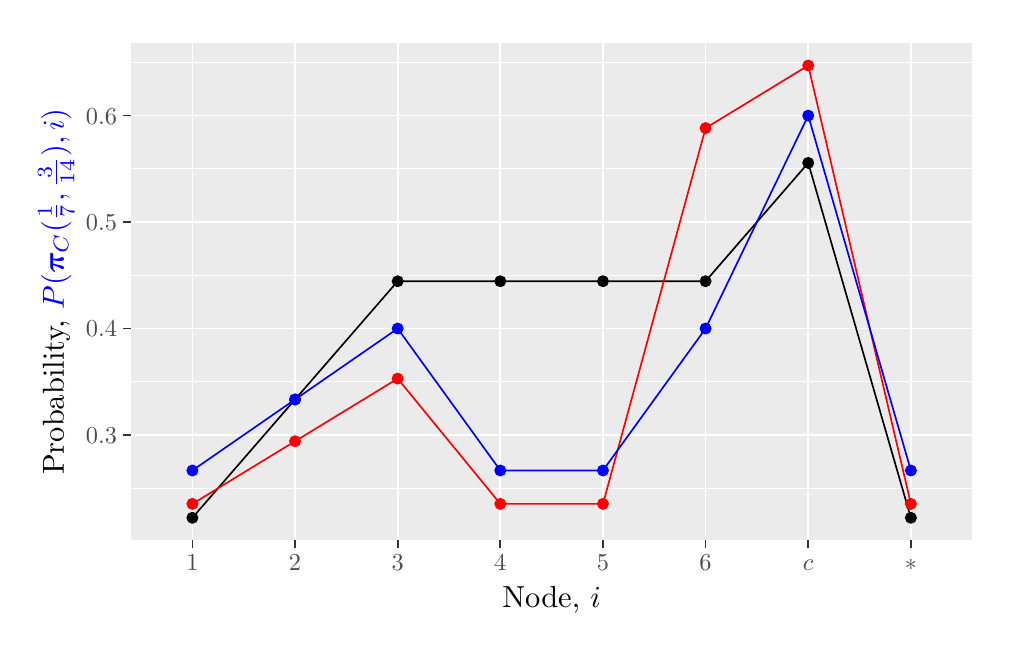
\begin{tikzpicture}[x=1pt,y=1pt]
\definecolor{fillColor}{RGB}{255,255,255}
\path[use as bounding box,fill=fillColor,fill opacity=0.00] (0,0) rectangle (346.90,216.81);
\begin{scope}
\path[clip] (  0.00,  0.00) rectangle (346.90,216.81);
\definecolor{drawColor}{RGB}{255,255,255}
\definecolor{fillColor}{RGB}{255,255,255}

\path[draw=drawColor,line width= 0.6pt,line join=round,line cap=round,fill=fillColor] (  0.00,  0.00) rectangle (346.90,216.81);
\end{scope}
\begin{scope}
\path[clip] ( 37.27, 31.53) rectangle (341.40,211.31);
\definecolor{fillColor}{gray}{0.92}

\path[fill=fillColor] ( 37.27, 31.53) rectangle (341.40,211.31);
\definecolor{drawColor}{RGB}{255,255,255}

\path[draw=drawColor,line width= 0.3pt,line join=round] ( 37.27, 50.39) --
	(341.40, 50.39);

\path[draw=drawColor,line width= 0.3pt,line join=round] ( 37.27, 88.86) --
	(341.40, 88.86);

\path[draw=drawColor,line width= 0.3pt,line join=round] ( 37.27,127.33) --
	(341.40,127.33);

\path[draw=drawColor,line width= 0.3pt,line join=round] ( 37.27,165.80) --
	(341.40,165.80);

\path[draw=drawColor,line width= 0.3pt,line join=round] ( 37.27,204.27) --
	(341.40,204.27);

\path[draw=drawColor,line width= 0.6pt,line join=round] ( 37.27, 69.62) --
	(341.40, 69.62);

\path[draw=drawColor,line width= 0.6pt,line join=round] ( 37.27,108.09) --
	(341.40,108.09);

\path[draw=drawColor,line width= 0.6pt,line join=round] ( 37.27,146.56) --
	(341.40,146.56);

\path[draw=drawColor,line width= 0.6pt,line join=round] ( 37.27,185.03) --
	(341.40,185.03);

\path[draw=drawColor,line width= 0.6pt,line join=round] ( 59.52, 31.53) --
	( 59.52,211.31);

\path[draw=drawColor,line width= 0.6pt,line join=round] ( 96.61, 31.53) --
	( 96.61,211.31);

\path[draw=drawColor,line width= 0.6pt,line join=round] (133.70, 31.53) --
	(133.70,211.31);

\path[draw=drawColor,line width= 0.6pt,line join=round] (170.79, 31.53) --
	(170.79,211.31);

\path[draw=drawColor,line width= 0.6pt,line join=round] (207.88, 31.53) --
	(207.88,211.31);

\path[draw=drawColor,line width= 0.6pt,line join=round] (244.96, 31.53) --
	(244.96,211.31);

\path[draw=drawColor,line width= 0.6pt,line join=round] (282.05, 31.53) --
	(282.05,211.31);

\path[draw=drawColor,line width= 0.6pt,line join=round] (319.14, 31.53) --
	(319.14,211.31);
\definecolor{drawColor}{RGB}{0,0,0}
\definecolor{fillColor}{RGB}{0,0,0}

\path[draw=drawColor,line width= 0.4pt,line join=round,line cap=round,fill=fillColor] ( 59.52, 39.70) circle (  1.96);

\path[draw=drawColor,line width= 0.4pt,line join=round,line cap=round,fill=fillColor] ( 96.61, 82.45) circle (  1.96);

\path[draw=drawColor,line width= 0.4pt,line join=round,line cap=round,fill=fillColor] (133.70,125.19) circle (  1.96);

\path[draw=drawColor,line width= 0.4pt,line join=round,line cap=round,fill=fillColor] (170.79,125.19) circle (  1.96);

\path[draw=drawColor,line width= 0.4pt,line join=round,line cap=round,fill=fillColor] (207.88,125.19) circle (  1.96);

\path[draw=drawColor,line width= 0.4pt,line join=round,line cap=round,fill=fillColor] (244.96,125.19) circle (  1.96);

\path[draw=drawColor,line width= 0.4pt,line join=round,line cap=round,fill=fillColor] (282.05,167.94) circle (  1.96);

\path[draw=drawColor,line width= 0.4pt,line join=round,line cap=round,fill=fillColor] (319.14, 39.70) circle (  1.96);

\path[draw=drawColor,line width= 0.6pt,line join=round] ( 59.52, 39.70) --
	( 96.61, 82.45) --
	(133.70,125.19) --
	(170.79,125.19) --
	(207.88,125.19) --
	(244.96,125.19) --
	(282.05,167.94) --
	(319.14, 39.70);
\definecolor{drawColor}{RGB}{255,0,0}
\definecolor{fillColor}{RGB}{255,0,0}

\path[draw=drawColor,line width= 0.4pt,line join=round,line cap=round,fill=fillColor] ( 59.52, 44.73) circle (  1.96);

\path[draw=drawColor,line width= 0.4pt,line join=round,line cap=round,fill=fillColor] ( 96.61, 67.36) circle (  1.96);

\path[draw=drawColor,line width= 0.4pt,line join=round,line cap=round,fill=fillColor] (133.70, 89.99) circle (  1.96);

\path[draw=drawColor,line width= 0.4pt,line join=round,line cap=round,fill=fillColor] (170.79, 44.73) circle (  1.96);

\path[draw=drawColor,line width= 0.4pt,line join=round,line cap=round,fill=fillColor] (207.88, 44.73) circle (  1.96);

\path[draw=drawColor,line width= 0.4pt,line join=round,line cap=round,fill=fillColor] (244.96,180.51) circle (  1.96);

\path[draw=drawColor,line width= 0.4pt,line join=round,line cap=round,fill=fillColor] (282.05,203.14) circle (  1.96);

\path[draw=drawColor,line width= 0.4pt,line join=round,line cap=round,fill=fillColor] (319.14, 44.73) circle (  1.96);

\path[draw=drawColor,line width= 0.6pt,line join=round] ( 59.52, 44.73) --
	( 96.61, 67.36) --
	(133.70, 89.99) --
	(170.79, 44.73) --
	(207.88, 44.73) --
	(244.96,180.51) --
	(282.05,203.14) --
	(319.14, 44.73);
\definecolor{drawColor}{RGB}{0,0,255}
\definecolor{fillColor}{RGB}{0,0,255}

\path[draw=drawColor,line width= 0.4pt,line join=round,line cap=round,fill=fillColor] ( 59.52, 56.80) circle (  1.96);

\path[draw=drawColor,line width= 0.4pt,line join=round,line cap=round,fill=fillColor] ( 96.61, 82.45) circle (  1.96);

\path[draw=drawColor,line width= 0.4pt,line join=round,line cap=round,fill=fillColor] (133.70,108.09) circle (  1.96);

\path[draw=drawColor,line width= 0.4pt,line join=round,line cap=round,fill=fillColor] (170.79, 56.80) circle (  1.96);

\path[draw=drawColor,line width= 0.4pt,line join=round,line cap=round,fill=fillColor] (207.88, 56.80) circle (  1.96);

\path[draw=drawColor,line width= 0.4pt,line join=round,line cap=round,fill=fillColor] (244.96,108.09) circle (  1.96);

\path[draw=drawColor,line width= 0.4pt,line join=round,line cap=round,fill=fillColor] (282.05,185.03) circle (  1.96);

\path[draw=drawColor,line width= 0.4pt,line join=round,line cap=round,fill=fillColor] (319.14, 56.80) circle (  1.96);

\path[draw=drawColor,line width= 0.6pt,line join=round] ( 59.52, 56.80) --
	( 96.61, 82.45) --
	(133.70,108.09) --
	(170.79, 56.80) --
	(207.88, 56.80) --
	(244.96,108.09) --
	(282.05,185.03) --
	(319.14, 56.80);
\end{scope}
\begin{scope}
\path[clip] (  0.00,  0.00) rectangle (346.90,216.81);
\definecolor{drawColor}{gray}{0.30}

\node[text=drawColor,anchor=base east,inner sep=0pt, outer sep=0pt, scale=  0.88] at ( 32.32, 66.59) {0.3};

\node[text=drawColor,anchor=base east,inner sep=0pt, outer sep=0pt, scale=  0.88] at ( 32.32,105.06) {0.4};

\node[text=drawColor,anchor=base east,inner sep=0pt, outer sep=0pt, scale=  0.88] at ( 32.32,143.53) {0.5};

\node[text=drawColor,anchor=base east,inner sep=0pt, outer sep=0pt, scale=  0.88] at ( 32.32,182.00) {0.6};
\end{scope}
\begin{scope}
\path[clip] (  0.00,  0.00) rectangle (346.90,216.81);
\definecolor{drawColor}{gray}{0.20}

\path[draw=drawColor,line width= 0.6pt,line join=round] ( 34.52, 69.62) --
	( 37.27, 69.62);

\path[draw=drawColor,line width= 0.6pt,line join=round] ( 34.52,108.09) --
	( 37.27,108.09);

\path[draw=drawColor,line width= 0.6pt,line join=round] ( 34.52,146.56) --
	( 37.27,146.56);

\path[draw=drawColor,line width= 0.6pt,line join=round] ( 34.52,185.03) --
	( 37.27,185.03);
\end{scope}
\begin{scope}
\path[clip] (  0.00,  0.00) rectangle (346.90,216.81);
\definecolor{drawColor}{gray}{0.20}

\path[draw=drawColor,line width= 0.6pt,line join=round] ( 59.52, 28.78) --
	( 59.52, 31.53);

\path[draw=drawColor,line width= 0.6pt,line join=round] ( 96.61, 28.78) --
	( 96.61, 31.53);

\path[draw=drawColor,line width= 0.6pt,line join=round] (133.70, 28.78) --
	(133.70, 31.53);

\path[draw=drawColor,line width= 0.6pt,line join=round] (170.79, 28.78) --
	(170.79, 31.53);

\path[draw=drawColor,line width= 0.6pt,line join=round] (207.88, 28.78) --
	(207.88, 31.53);

\path[draw=drawColor,line width= 0.6pt,line join=round] (244.96, 28.78) --
	(244.96, 31.53);

\path[draw=drawColor,line width= 0.6pt,line join=round] (282.05, 28.78) --
	(282.05, 31.53);

\path[draw=drawColor,line width= 0.6pt,line join=round] (319.14, 28.78) --
	(319.14, 31.53);
\end{scope}
\begin{scope}
\path[clip] (  0.00,  0.00) rectangle (346.90,216.81);
\definecolor{drawColor}{gray}{0.30}

\node[text=drawColor,anchor=base,inner sep=0pt, outer sep=0pt, scale=  0.88] at ( 59.52, 20.52) {$1$};

\node[text=drawColor,anchor=base,inner sep=0pt, outer sep=0pt, scale=  0.88] at ( 96.61, 20.52) {$2$};

\node[text=drawColor,anchor=base,inner sep=0pt, outer sep=0pt, scale=  0.88] at (133.70, 20.52) {$3$};

\node[text=drawColor,anchor=base,inner sep=0pt, outer sep=0pt, scale=  0.88] at (170.79, 20.52) {$4$};

\node[text=drawColor,anchor=base,inner sep=0pt, outer sep=0pt, scale=  0.88] at (207.88, 20.52) {$5$};

\node[text=drawColor,anchor=base,inner sep=0pt, outer sep=0pt, scale=  0.88] at (244.96, 20.52) {$6$};

\node[text=drawColor,anchor=base,inner sep=0pt, outer sep=0pt, scale=  0.88] at (282.05, 20.52) {$c$};

\node[text=drawColor,anchor=base,inner sep=0pt, outer sep=0pt, scale=  0.88] at (319.14, 20.52) {$*$};
\end{scope}
\begin{scope}
\path[clip] (  0.00,  0.00) rectangle (346.90,216.81);
\definecolor{drawColor}{RGB}{0,0,0}

\node[text=drawColor,anchor=base,inner sep=0pt, outer sep=0pt, scale=  1.10] at (189.33,  7.44) {Node, $i$};
\end{scope}
\begin{scope}
\path[clip] (  0.00,  0.00) rectangle (346.90,216.81);
\definecolor{drawColor}{RGB}{0,0,0}

\node[text=drawColor,rotate= 90.00,anchor=base,inner sep=0pt, outer sep=0pt, scale=  1.10] at ( 13.08,121.42) {Probability, \textcolor{blue}{$P(\bm{\pi}_{C}(\frac{1}{7},\frac{3}{14}),i)$}};
\end{scope}
\end{tikzpicture}

\end{center}
\caption{Interception probabilities of $S^5_{4}$ when $m=4$, with the \textcolor{red}{red Probabilities showing the Naive Improvement Policy $\bm{\pi}_{N} \left(\frac{2}{17},\frac{6}{17} \right)$} and the \textcolor{blue}{blue Probabilities showing the Choosing Improvement Policy $\bm{\pi}_{C} \left(\frac{1}{7},\frac{3}{14} \right)$}.}
\end{myfigure}

It is conjectured in our future work (see section \ref{Section:Further solutions for elongated trees}) that the bound $V \geq \frac{2m}{2(n+k)+m(1+\frac{n-1}{\hat{m}})}$ is used in the region of $m < 2(k+1)$. When $m$ is even this bound becomes $V \geq \frac{2m}{2(2n+k-1)+m}$ which we will conjecture is tight with a multitude of attack strategies, however when $m$ is odd due to the half-length, $\hat{m} \equiv \floor{\frac{m}{2}}$, it makes the bound higher than when $m$ is even, which will not be tight. We suggest some slight alteration when $m$ is odd, but have to drop the use of end-covering cycles (we leave this idea to section \ref{Section:Further solutions for elongated trees})

We will now deal with the case of $m \leq 2(n-1)$, so that all $*$'s nodes cannot be covered in one end-covering cycle. First looking at the $m=2k+1,2k$,  we notice that by simplification of $S^{k}_{n}$ into $L_{k+1}$ and $S_{n-1}$ we get the bound $V \geq \frac{1}{1+\frac{2(n-1)}{m}}=\frac{m}{m+2(n-1)}$.

When $m=2k+1$ we can propose an attack that `augments' the time-delayed which simply removes one attack placed at $1$. That is to place attacks at node $1$ starting at times, $\tau,...,\tau+2k$ and $*$ nodes starting at times $\tau+k,\tau+k+1$ (equally we could use $\tau+k-1,\tau+k$) all with equal probability. Similarly if $m=2k$ we augment it to node $1$ at times $\tau,...,\tau+2k-1$ and $*$ nodes at times $\tau+k-1,\tau+k$ all with equal probability.

\begin{lemma}
Using the `augmented' time-delayed we propose the attacker can get a bound of $V \leq \frac{m}{m+2(n-1)}$ and hence $V(S_{n}^{k})=\frac{m}{m+2(n-1)}$ for $m=2k+1,2k$
\end{lemma}

The idea of the proof for the `augmented' time-delayed attack is the same as the time-delayed attack, but with a reduced number of attacks at node $1$, to make sure the patroller can only get $m$ by waiting here. No significant alteration to the proof takes place.

We leave the rest of the idea to solve in the region $m < 2(k+1)$ to \ref{Section:Further solutions for elongated trees}, but respect that it may be difficult and careful consideration of attacker strategies may need to be taken when the random oscillation is not the best strategy for the patroller. This is analagous to the situtation in the region of $S_{5}$ for the line (see section 5 in \cite{Lin2013}).

\subsection{Generalising the star graph}
For now we will set aside the difficulty with the elongated star and look at generalising it, in which we can solve for values of $m$ which match the random oscillation. We generalise further by allowing a general star graph to have all external nodes any distance from the centre node, again performed by subdivision of the edge an appropriate number of times.

\begin{definition}[General star graph]
The \textit{general star graph}, $S^{\bm{k}}_{n}$ ($\bm{k} \in \mathbb{N}^{h}$) is made from $S_{n}$, by performing subdivision on $h$ of the  initial edges each repeated $k_{i}$ for each edge for $i=1,...,h$ . 
\end{definition}

\begin{note}
For ease of notation we will use the above format, but will understand that using $k_{i}=0$ is a valid construction, so we can imagine that $\bm{k} \in \mathbb{N}^n$.
For ease of notation we will also define define $ |\bm{k}| \equiv \sum\limits_{i=0}^{i=h} k_{i}$ and $ k_{\max} \equiv \max\limits_{i=1,2,..,h} k_{i}$.
\end{note}

The labelling will be done as in figure \ref{Figure:Example of generalised labelling} and note that all nodes with the same label are symmetric and must be treated as such. We will refer to the branch made by $k_{i}$ subdivisions of the edge as the $i$\textsuperscript{th} branch, which is made up of the nodes $n_{j,i}$ for $j=1,...,k_{i}+1$, so $n_{j,i}$ is $j$\textsuperscript{th} node on $i$\textsuperscript{th} branch).

\begin{myfigure}
\begin{center}
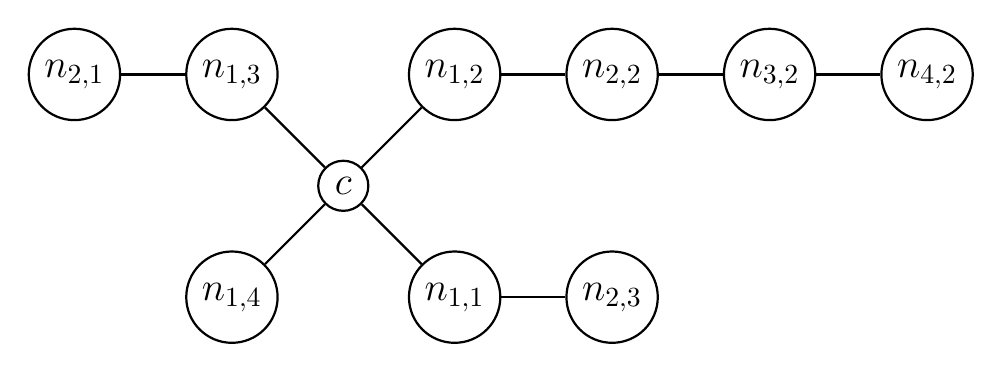
\begin{tikzpicture}[-,auto,node distance=2cm,
                    thick,main node/.style={circle,draw,font=\sffamily\Large\bfseries}]

  \node[main node] (1) {$c$};
  \node[main node] (2) [below left of=1] {$n_{1,4}$};
  \node[main node] (3) [below right of=1] {$n_{1,1}$};
  \node[main node] (4) [above left of=1] {$n_{1,3}$};
  \node[main node] (5) [above right of=1] {$n_{1,2}$};
  \node[main node] (6) [right of=5]  {$n_{2,2}$};
  \node[main node] (7) [right of=6]  {$n_{3,2}$};
  \node[main node] (8) [right of=7]  {$n_{4,2}$};
  \node[main node] (9) [left of=4] {$n_{2,1}$};
  \node[main node] (10) [right of=3] {$n_{2,3}$};
  
  \path[every node/.style={font=\sffamily}]
    (1) edge  (2)
    edge(3)
    edge(4)
    edge(5)
    (5) edge (6)
    (6) edge (7)
    (7) edge (8)
    (9) edge (4)
    (10) edge (3);
    
\end{tikzpicture}
\end{center}
\caption{Labelling of $S^{1,3,1}_{4}$.}
\label{Figure:Example of generalised labelling}
\end{myfigure}

To start our analysis of this graph, we will look at an expanded graph which can be simplified down to our general star graph. Consider the cyclic graph $C_{2(n+|k|)}$, this can simplified to $S^{\bm{k}}_{n}$ by node identification. The identification mapping is analogous to that of the elongated star graph's simplification from a cyclic graph; Internal branch nodes are seen twice and the centre node is seen on every return, so the cycle graph can be made from this construction as in the example in figure \ref{Figure:Example of simplification to general star graph}.

The mapping is done as such:
\begin{itemize}
\item The centre is identified from nodes $1,1+2(k_{1}+1),1+2(\sum\limits_{i=1}^{2} (k_{i}+1)),...,1+2(\sum\limits_{i=1}^{h}(k_{i}+1),1+2(|k|+h)+2),...,1+2(|k|+h)+2(n-h)$

\item The first branch is identified from the nodes between $2$ and $2(k_{1}+1)$ (Inclusive). $n_{1,i}$ for $i=1,...,k_{1}$ are identified by the two nodes $i+1$ and $2k_{1}+3-i$ , the node $n_{1,k_{1}+1}$ is identified by the one node $k_{1}+2$.

\item The $j$\textsuperscript{th} branch is identified from nodes between $2(\sum\limits_{i=1}^{j-1} (k_{i}+1)))$ and $2(\sum\limits_{i=1}^{j} (k_{i}+1)))$ (Inclusive). $n_{j,i}$ for $i=1,....,k_{j}$ are identified by the two nodes $2(\sum\limits_{i=1}^{j-1} (k_{i}+1)))+(i-1)$ and $2(\sum\limits_{i=1}^{j} (k_{i}+1)))-(i-1)$ , the node $n_{j,k_{j}+1}$ is identified by the one node $2(\sum\limits_{i=1}^{j-1} (k_{i}+1)))+k_{j}$.
\end{itemize}

This simplification mapping gives rise to the general random oscillation strategy (analogous to random oscillation on the elongated star).

\begin{definition}[General random oscillation]
The \textit{oscillation} on $S^{\bm{k}}_{n}$ is any embedded Hamiltonian patrol on $C_{2(n+|k|)}$ under the simplification above. The \textit{random oscillation} on $S^{\bm{k}}_{n}$ is the embedded random Hamiltonian patrol on $C_{2(n+|k|)}$ under the simplification above.
\end{definition}

\begin{lemma}
For $m < 2(n+|k|)$ following the random oscillation
$$V(S^{\bm{k}}_{n}) \geq V(C_{2(n+|k|)})=\frac{m}{2(n+|k|)}$$
and if $m \geq 2(n+|k|)$ then $V(S^{\bm{k}}_{n})=1$, achieved by any oscillation. 
\end{lemma}

The proof is straight forward by the application of the simplification (Lemma 1 (4) in \cite{Alpern2011}) and the Hamiltonian solution(Theorem 13 (1) in \cite{Alpern2011}).

\begin{myfigure}
\begin{center}
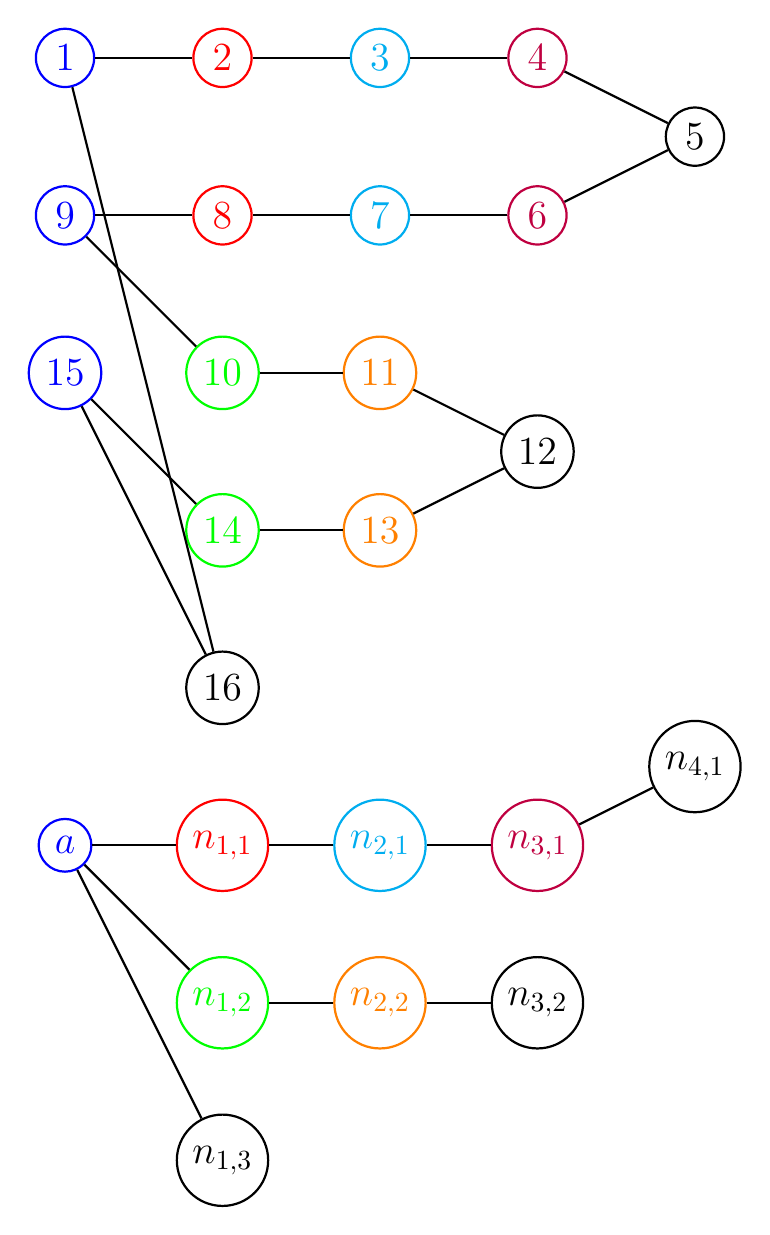
\begin{tikzpicture}[-,auto,node distance=2cm,
                    thick,main node/.style={circle,draw,font=\sffamily\Large\bfseries}]

  \node[main node,color=blue] (1) {$1$};
  \node[main node,color=blue] (2) [below of=1] {$9$};
  \node[main node,color=blue] (3) [below of=2] {$15$};
  \node[main node,color=red] (4) [right of=1] {$2$};
  \node[main node,color=red] (5) [right of=2]  {$8$};
  \node[main node,color=green] (6) [right of=3]  {$10$};
  \node[main node,color=green] (7) [below of=6]  {$14$};
  \node[main node] (13) [below of=7] {$16$};
  \node[main node,color=cyan] (8) [right of=4]  {$3$};
  \node[main node,color=purple] (9) [right of=8]  {$4$};
  \node[main node,color=cyan] (10) [right of=5]  {$7$};
  \node[main node,color=purple] (11) [right of=10]  {$6$};
  \node[main node] at (8,-1) (12)  {$5$};
  \node[main node,color=orange] (14) [right of=6] {$11$};
  \node[main node,color=orange] (15) [right of=7] {$13$};
  \node[main node] at (6,-5) (16) {$12$};

  \path[every node/.style={font=\sffamily}]
    (1) edge  (4)
    (2) edge  (5)
        edge  (6)
    (3) edge  (7)
    
    (4) edge (8)
    (13) edge (3)
    (13) edge (1)
    (8) edge (9)
    (9) edge (12)
    (12) edge (11)
    (11) edge (10)
    (10) edge (5)
    (6) edge (14)
    (7) edge (15)
    (14) edge (16)
    (15) edge (16);
  
  \node[main node,color=blue] (13) [below of=3,node distance=6cm] {$a$};
  \node[main node,color=red] (14) [right of=13] {$n_{1,1}$};
  \node[main node,color=green] (15) [below of=14] {$n_{1,2}$};
  \node[main node] (16) [below of=15] {$n_{1,3}$};
  \node[main node,color=cyan] (17) [right of=14] {$n_{2,1}$};
  \node[main node,color=purple] (18) [right of=17] {$n_{3,1}$};
  \node[main node] at (8,-9) (19) {$n_{4,1}$};      
  \node[main node,color=orange] (20) [right of=15] {$n_{2,2}$};
  \node[main node] (21) [right of=20] {$n_{3,2}$}; 
   
   \path[every node/.style={font=\sffamily}]
   (13) edge (14)
   edge (15)
   edge (16)
   (14) edge (17)
   (17) edge (18)
   (18) edge (19)
   (15) edge (20)
   (20) edge (21);
  
\end{tikzpicture}
\end{center}
\caption{Simplification of $C_{16}$ to $S^{3,2}_{3}$.}
\label{Figure:Example of simplification to general star graph}
\end{myfigure}

We will match the oscillation bound of $\frac{m}{2(n+|k|)}$, by further extending the time-delayed attack into the type-delayed attack, which will consider the length of the branches as the key to spacing out the attacks in time.

\begin{definition}[Node types]
A \textit{type} $i$ node, is an external node which has been extended $i$ times, that is the branch length. Then $k_{\max}$ is the maximum node type for $S_{n}^{\bm{k}}$.
\end{definition}

\begin{definition}[Type-delayed attack]
Let the \textit{type-delayed attack}, be the attack that attacks at a type $i$ node with probability $\frac{i+1}{\denominator}$ $\forall \, i$. For a fixed attack interval $I$, the attacks at a type $i$ node choose an interval from the following with equal probability: $I+(k_{max}-i),I+(k_{max}-i)+1,...,I+k_{max}+i+1$ $\forall \, i$ (i.e starting attacks at a type $i$ node at times $\tau+(k_{max}-i)+1,...,\tau+(k_{max}+i)+1$).
\end{definition}

A diagram showing how potential attacks are spaced out in time, for each node of a given type, can be seen in figure \ref{Figure:Time spacing of the type-delayed attack}.

\begin{myfigure}
\begin{center}
\resizebox{\linewidth}{!}{
\begin{tikzpicture}
 %Drawing Bottom Axis
 \draw[->] (-7,0) -- (7,0);
 \node (timelabel) [shift={(0.2,0)}] at (7,0) {$t$};
 
 
 \draw (-6.5,0.2) -- (-6.5,-0.2);
 \draw (6.5,0.2) -- (6.5,-0.2);
 
 \node (labelc1) at (-6.5,-0.5) {$\tau$};
 \node (labelc2) at (6.5,-0.5) {$\tau+2k_{max}+1$};
 
 \node[cross=5pt,red] (c1) at (-6.5,0.5) {};
 \node[cross=5pt,red] (c2) at (6.5,0.5) {};
 \draw[dashed] (c1) -- (c2);
 \node (linelabel1) at (-8,0.5) {Type $k_{max}$};
 
 
  \draw (-6,0.2) -- (-6,-0.2);
 \draw (6,0.2) -- (6,-0.2);
 
 %\node (labelc1) at (-5.5,-0.5) {$\tau+1$};
 %\node (labelc2) at (5.5,-0.5) {$\tau+2k_{max}-1$};
 
 \node[cross=5pt,red] (c1) at (-6,1.5) {};
 \node[cross=5pt,red] (c2) at (6,1.5) {};
 \draw[dashed] (c1) -- (c2);
 \node (linelabel1) at (-7.5,1.5) {Type $k_{max}-1$};
 
 
 
 \draw[decorate sep={2mm}{4mm},fill] (0,3.5) -- (0,2);

  \draw (-1.5,0.2) -- (-1.5,-0.2);
 \draw (1.5,0.2) -- (1.5,-0.2);
 
 %\node (labelc1) at (-5.5,-0.5) {$\tau+1$};
 %\node (labelc2) at (5.5,-0.5) {$\tau+2k_{max}-1$};
 
 \node[cross=5pt,red] (c1) at (-1.5,4) {};
 \node[cross=5pt,red] (c2) at (1.5,4) {};
 \draw[dashed] (c1) -- (c2);
 \node (linelabel1) at (-2.3,4) {Type $1$};
 
 \draw (-1,0.2) -- (-1,-0.2);
 \draw (1,0.2) -- (1,-0.2);
 
  \node (labelc3) at (-1,-0.5) {$\tau+k_{max}$};
 \node (labelc4) at (1,-0.5) {$\tau+k_{max}+1$};
 
 \node[cross=5pt,red] (c3) at (-1,5) {};
 \node[cross=5pt,red] (c4) at (1,5) {};
 \draw[dashed] (c3) -- (c4);
 \node (linelabel1) at (-1.9,5) {Type $0$}; 

\end{tikzpicture}
}
\end{center}
\caption{Time spacing of the type-delayed attack.}
\label{Figure:Time spacing of the type-delayed attack}
\end{myfigure}

\begin{theorem}
When $T \geq m+2k_{max}$, the upper bound is
$$V(S_{n}^{\bm{k}}) \leq \max \left\{ \frac{k_{max}+1}{\denominator} , \frac{m}{2 \left( \denominator \right)} \right\}$$
guaranteed by the type-delayed attack.
\end{theorem}

We leave the proof of this

\begin{corollary}[Solution in $m \geq 2(k_{max}+1)$]
When $T \geq m+2k_{max}$, by the attack using the type-delayed attack and the patroller using the random oscillation we achieve the value, when $2(k_{max}+1) \leq m \leq 2(n+|\bm{k}|)$,
$$V= \frac{m}{2(n+|\bm{k}|)} $$
and when $m > 2(n+|\bm{k}|)$ then $V=1$.
\end{corollary}

\begin{myfigure}
\begin{center}
% Created by tikzDevice version 0.10.1 on 2018-06-27 15:40:42
% !TEX encoding = UTF-8 Unicode
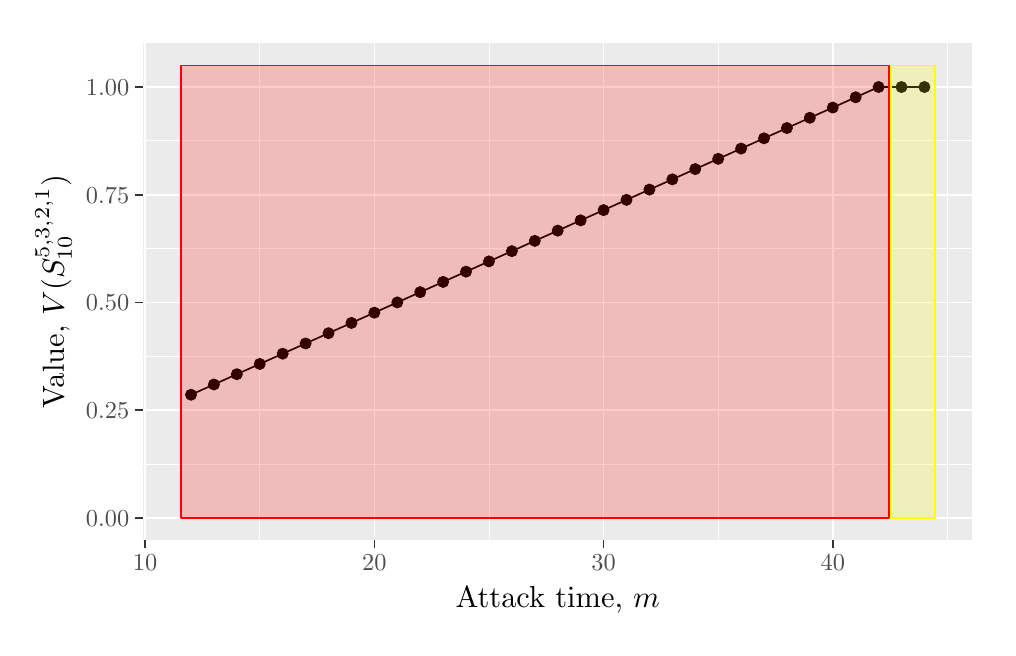
\begin{tikzpicture}[x=1pt,y=1pt]
\definecolor{fillColor}{RGB}{255,255,255}
\path[use as bounding box,fill=fillColor,fill opacity=0.00] (0,0) rectangle (346.90,216.81);
\begin{scope}
\path[clip] (  0.00,  0.00) rectangle (346.90,216.81);
\definecolor{drawColor}{RGB}{255,255,255}
\definecolor{fillColor}{RGB}{255,255,255}

\path[draw=drawColor,line width= 0.6pt,line join=round,line cap=round,fill=fillColor] (  0.00,  0.00) rectangle (346.90,216.81);
\end{scope}
\begin{scope}
\path[clip] ( 41.67, 31.53) rectangle (341.40,211.31);
\definecolor{fillColor}{gray}{0.92}

\path[fill=fillColor] ( 41.67, 31.53) rectangle (341.40,211.31);
\definecolor{drawColor}{RGB}{255,255,255}

\path[draw=drawColor,line width= 0.3pt,line join=round] ( 41.67, 59.16) --
	(341.40, 59.16);

\path[draw=drawColor,line width= 0.3pt,line join=round] ( 41.67, 98.07) --
	(341.40, 98.07);

\path[draw=drawColor,line width= 0.3pt,line join=round] ( 41.67,136.99) --
	(341.40,136.99);

\path[draw=drawColor,line width= 0.3pt,line join=round] ( 41.67,175.90) --
	(341.40,175.90);

\path[draw=drawColor,line width= 0.3pt,line join=round] ( 83.86, 31.53) --
	( 83.86,211.31);

\path[draw=drawColor,line width= 0.3pt,line join=round] (166.68, 31.53) --
	(166.68,211.31);

\path[draw=drawColor,line width= 0.3pt,line join=round] (249.51, 31.53) --
	(249.51,211.31);

\path[draw=drawColor,line width= 0.3pt,line join=round] (332.33, 31.53) --
	(332.33,211.31);

\path[draw=drawColor,line width= 0.6pt,line join=round] ( 41.67, 39.70) --
	(341.40, 39.70);

\path[draw=drawColor,line width= 0.6pt,line join=round] ( 41.67, 78.62) --
	(341.40, 78.62);

\path[draw=drawColor,line width= 0.6pt,line join=round] ( 41.67,117.53) --
	(341.40,117.53);

\path[draw=drawColor,line width= 0.6pt,line join=round] ( 41.67,156.44) --
	(341.40,156.44);

\path[draw=drawColor,line width= 0.6pt,line join=round] ( 41.67,195.36) --
	(341.40,195.36);

\path[draw=drawColor,line width= 0.6pt,line join=round] ( 42.45, 31.53) --
	( 42.45,211.31);

\path[draw=drawColor,line width= 0.6pt,line join=round] (125.27, 31.53) --
	(125.27,211.31);

\path[draw=drawColor,line width= 0.6pt,line join=round] (208.10, 31.53) --
	(208.10,211.31);

\path[draw=drawColor,line width= 0.6pt,line join=round] (290.92, 31.53) --
	(290.92,211.31);
\definecolor{drawColor}{RGB}{0,0,0}
\definecolor{fillColor}{RGB}{0,0,0}

\path[draw=drawColor,line width= 0.4pt,line join=round,line cap=round,fill=fillColor] (315.76,195.36) circle (  1.96);

\path[draw=drawColor,line width= 0.4pt,line join=round,line cap=round,fill=fillColor] (324.04,195.36) circle (  1.96);

\path[draw=drawColor,line width= 0.4pt,line join=round,line cap=round,fill=fillColor] ( 59.02, 84.17) circle (  1.96);

\path[draw=drawColor,line width= 0.4pt,line join=round,line cap=round,fill=fillColor] ( 67.30, 87.88) circle (  1.96);

\path[draw=drawColor,line width= 0.4pt,line join=round,line cap=round,fill=fillColor] ( 75.58, 91.59) circle (  1.96);

\path[draw=drawColor,line width= 0.4pt,line join=round,line cap=round,fill=fillColor] ( 83.86, 95.29) circle (  1.96);

\path[draw=drawColor,line width= 0.4pt,line join=round,line cap=round,fill=fillColor] ( 92.15, 99.00) circle (  1.96);

\path[draw=drawColor,line width= 0.4pt,line join=round,line cap=round,fill=fillColor] (100.43,102.70) circle (  1.96);

\path[draw=drawColor,line width= 0.4pt,line join=round,line cap=round,fill=fillColor] (108.71,106.41) circle (  1.96);

\path[draw=drawColor,line width= 0.4pt,line join=round,line cap=round,fill=fillColor] (116.99,110.12) circle (  1.96);

\path[draw=drawColor,line width= 0.4pt,line join=round,line cap=round,fill=fillColor] (125.27,113.82) circle (  1.96);

\path[draw=drawColor,line width= 0.4pt,line join=round,line cap=round,fill=fillColor] (133.56,117.53) circle (  1.96);

\path[draw=drawColor,line width= 0.4pt,line join=round,line cap=round,fill=fillColor] (141.84,121.24) circle (  1.96);

\path[draw=drawColor,line width= 0.4pt,line join=round,line cap=round,fill=fillColor] (150.12,124.94) circle (  1.96);

\path[draw=drawColor,line width= 0.4pt,line join=round,line cap=round,fill=fillColor] (158.40,128.65) circle (  1.96);

\path[draw=drawColor,line width= 0.4pt,line join=round,line cap=round,fill=fillColor] (166.68,132.35) circle (  1.96);

\path[draw=drawColor,line width= 0.4pt,line join=round,line cap=round,fill=fillColor] (174.97,136.06) circle (  1.96);

\path[draw=drawColor,line width= 0.4pt,line join=round,line cap=round,fill=fillColor] (183.25,139.77) circle (  1.96);

\path[draw=drawColor,line width= 0.4pt,line join=round,line cap=round,fill=fillColor] (191.53,143.47) circle (  1.96);

\path[draw=drawColor,line width= 0.4pt,line join=round,line cap=round,fill=fillColor] (199.81,147.18) circle (  1.96);

\path[draw=drawColor,line width= 0.4pt,line join=round,line cap=round,fill=fillColor] (208.10,150.88) circle (  1.96);

\path[draw=drawColor,line width= 0.4pt,line join=round,line cap=round,fill=fillColor] (216.38,154.59) circle (  1.96);

\path[draw=drawColor,line width= 0.4pt,line join=round,line cap=round,fill=fillColor] (224.66,158.30) circle (  1.96);

\path[draw=drawColor,line width= 0.4pt,line join=round,line cap=round,fill=fillColor] (232.94,162.00) circle (  1.96);

\path[draw=drawColor,line width= 0.4pt,line join=round,line cap=round,fill=fillColor] (241.22,165.71) circle (  1.96);

\path[draw=drawColor,line width= 0.4pt,line join=round,line cap=round,fill=fillColor] (249.51,169.41) circle (  1.96);

\path[draw=drawColor,line width= 0.4pt,line join=round,line cap=round,fill=fillColor] (257.79,173.12) circle (  1.96);

\path[draw=drawColor,line width= 0.4pt,line join=round,line cap=round,fill=fillColor] (266.07,176.83) circle (  1.96);

\path[draw=drawColor,line width= 0.4pt,line join=round,line cap=round,fill=fillColor] (274.35,180.53) circle (  1.96);

\path[draw=drawColor,line width= 0.4pt,line join=round,line cap=round,fill=fillColor] (282.63,184.24) circle (  1.96);

\path[draw=drawColor,line width= 0.4pt,line join=round,line cap=round,fill=fillColor] (290.92,187.94) circle (  1.96);

\path[draw=drawColor,line width= 0.4pt,line join=round,line cap=round,fill=fillColor] (299.20,191.65) circle (  1.96);

\path[draw=drawColor,line width= 0.4pt,line join=round,line cap=round,fill=fillColor] (307.48,195.36) circle (  1.96);

\path[draw=drawColor,line width= 0.6pt,line join=round] ( 59.02, 84.17) --
	( 67.30, 87.88) --
	( 75.58, 91.59) --
	( 83.86, 95.29) --
	( 92.15, 99.00) --
	(100.43,102.70) --
	(108.71,106.41) --
	(116.99,110.12) --
	(125.27,113.82) --
	(133.56,117.53) --
	(141.84,121.24) --
	(150.12,124.94) --
	(158.40,128.65) --
	(166.68,132.35) --
	(174.97,136.06) --
	(183.25,139.77) --
	(191.53,143.47) --
	(199.81,147.18) --
	(208.10,150.88) --
	(216.38,154.59) --
	(224.66,158.30) --
	(232.94,162.00) --
	(241.22,165.71) --
	(249.51,169.41) --
	(257.79,173.12) --
	(266.07,176.83) --
	(274.35,180.53) --
	(282.63,184.24) --
	(290.92,187.94) --
	(299.20,191.65) --
	(307.48,195.36) --
	(315.76,195.36) --
	(324.04,195.36);
\definecolor{drawColor}{RGB}{255,255,0}
\definecolor{fillColor}{RGB}{255,255,0}

\path[draw=drawColor,line width= 0.6pt,line join=round,fill=fillColor,fill opacity=0.20] (312.04, 39.70) rectangle (327.77,203.14);
\definecolor{drawColor}{RGB}{255,0,0}
\definecolor{fillColor}{RGB}{255,0,0}

\path[draw=drawColor,line width= 0.6pt,line join=round,fill=fillColor,fill opacity=0.20] ( 55.29, 39.70) rectangle (311.21,203.14);
\end{scope}
\begin{scope}
\path[clip] (  0.00,  0.00) rectangle (346.90,216.81);
\definecolor{drawColor}{gray}{0.30}

\node[text=drawColor,anchor=base east,inner sep=0pt, outer sep=0pt, scale=  0.88] at ( 36.72, 36.67) {0.00};

\node[text=drawColor,anchor=base east,inner sep=0pt, outer sep=0pt, scale=  0.88] at ( 36.72, 75.59) {0.25};

\node[text=drawColor,anchor=base east,inner sep=0pt, outer sep=0pt, scale=  0.88] at ( 36.72,114.50) {0.50};

\node[text=drawColor,anchor=base east,inner sep=0pt, outer sep=0pt, scale=  0.88] at ( 36.72,153.41) {0.75};

\node[text=drawColor,anchor=base east,inner sep=0pt, outer sep=0pt, scale=  0.88] at ( 36.72,192.33) {1.00};
\end{scope}
\begin{scope}
\path[clip] (  0.00,  0.00) rectangle (346.90,216.81);
\definecolor{drawColor}{gray}{0.20}

\path[draw=drawColor,line width= 0.6pt,line join=round] ( 38.92, 39.70) --
	( 41.67, 39.70);

\path[draw=drawColor,line width= 0.6pt,line join=round] ( 38.92, 78.62) --
	( 41.67, 78.62);

\path[draw=drawColor,line width= 0.6pt,line join=round] ( 38.92,117.53) --
	( 41.67,117.53);

\path[draw=drawColor,line width= 0.6pt,line join=round] ( 38.92,156.44) --
	( 41.67,156.44);

\path[draw=drawColor,line width= 0.6pt,line join=round] ( 38.92,195.36) --
	( 41.67,195.36);
\end{scope}
\begin{scope}
\path[clip] (  0.00,  0.00) rectangle (346.90,216.81);
\definecolor{drawColor}{gray}{0.20}

\path[draw=drawColor,line width= 0.6pt,line join=round] ( 42.45, 28.78) --
	( 42.45, 31.53);

\path[draw=drawColor,line width= 0.6pt,line join=round] (125.27, 28.78) --
	(125.27, 31.53);

\path[draw=drawColor,line width= 0.6pt,line join=round] (208.10, 28.78) --
	(208.10, 31.53);

\path[draw=drawColor,line width= 0.6pt,line join=round] (290.92, 28.78) --
	(290.92, 31.53);
\end{scope}
\begin{scope}
\path[clip] (  0.00,  0.00) rectangle (346.90,216.81);
\definecolor{drawColor}{gray}{0.30}

\node[text=drawColor,anchor=base,inner sep=0pt, outer sep=0pt, scale=  0.88] at ( 42.45, 20.52) {10};

\node[text=drawColor,anchor=base,inner sep=0pt, outer sep=0pt, scale=  0.88] at (125.27, 20.52) {20};

\node[text=drawColor,anchor=base,inner sep=0pt, outer sep=0pt, scale=  0.88] at (208.10, 20.52) {30};

\node[text=drawColor,anchor=base,inner sep=0pt, outer sep=0pt, scale=  0.88] at (290.92, 20.52) {40};
\end{scope}
\begin{scope}
\path[clip] (  0.00,  0.00) rectangle (346.90,216.81);
\definecolor{drawColor}{RGB}{0,0,0}

\node[text=drawColor,anchor=base,inner sep=0pt, outer sep=0pt, scale=  1.10] at (191.53,  7.44) {Attack time, $m$};
\end{scope}
\begin{scope}
\path[clip] (  0.00,  0.00) rectangle (346.90,216.81);
\definecolor{drawColor}{RGB}{0,0,0}

\node[text=drawColor,rotate= 90.00,anchor=base,inner sep=0pt, outer sep=0pt, scale=  1.10] at ( 13.08,121.42) {Value, $V(S_{ 10 }^{ 5, 3, 2, 1 })$};
\end{scope}
\end{tikzpicture}

\end{center}
\caption{The value of the general star graph, $S_{10}^{5,3,2,1}$.}
\end{myfigure}

Just like in the elognated star graph, we have solved the problem for the analogous regions to $S_{1}$ and $S_{2}$ for the line. As in the elongated star graph we expect a multitude of issues moving to the region of $m < 2(k_{\max}+1)$, so for now we shall move onto an even more general result.

\subsection{Joining star graphs by centralised connections}

We now look at connecting by their centres the generalised star (with branches).

\begin{definition}
We define the \textit{multi general p-star graph}, $(s_{n_{1}}^{\bm{k}_{p}},...,S_{n_{}}^{\bm{k}_{p}}) \equiv \bigodot\limits_{i=1}^{p} S_{n_{i}}^{\bm{k}_{i}}$, to be the p star graphs, $S_{n_{i}}^{\bm{k}_{i}}$ initially with disconnected centres which are now made adjacent by the introduction of connections between each combination of centres (i.e the complete graph of centres).
\end{definition}

\begin{myfigure}
\begin{center}
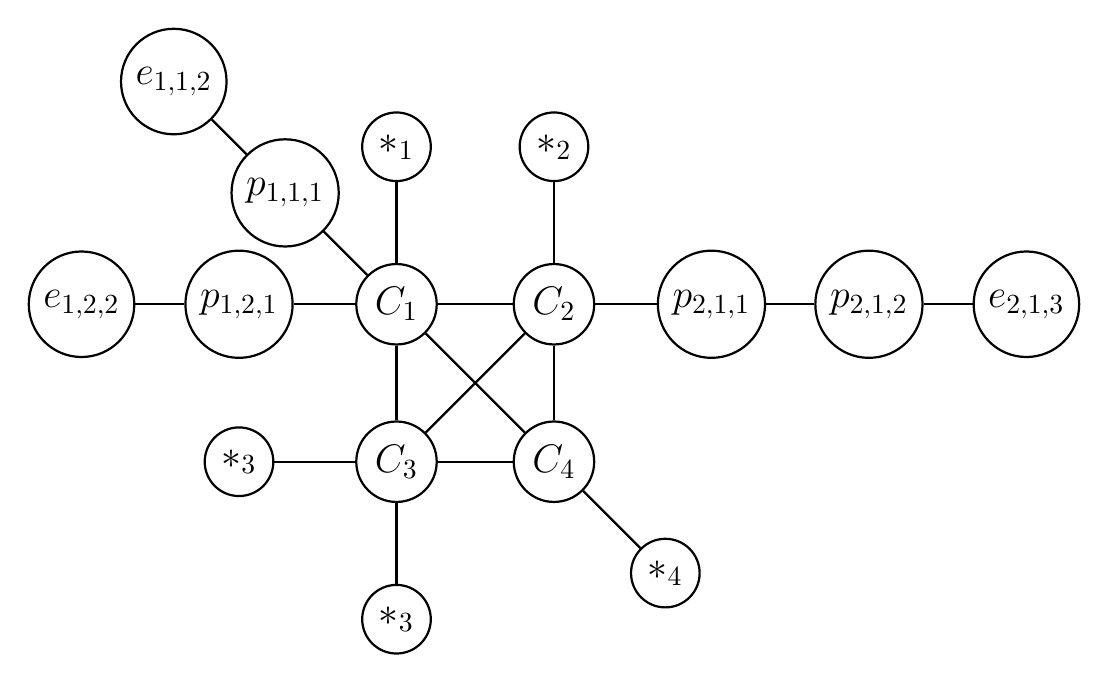
\begin{tikzpicture}[-,auto,node distance=2cm,
                    thick,main node/.style={circle,draw,font=\sffamily\Large\bfseries}]

 \node[main node] (c1) {$C_{1}$};
 \node[main node] (1) [above of=c1] {$*_{1}$};
 \node[main node] (2) [above left of=c1] {$p_{1,1,1}$};
 \node[main node] (3) [left of=c1] {$p_{1,2,1}$};
 \node[main node] (4) [above left of=2] {$e_{1,1,2}$};
 \node[main node] (5) [left of=3] {$e_{1,2,2}$};
  
 \path
 (c1) edge (1)
      edge (2)
      edge (3)
  (2) edge (4)
  (3) edge (5);
 
 \node[main node] (c2) [right of=c1] {$C_{2}$};
 \node[main node] (6) [above of=c2] {$*_{2}$};
 \node[main node] (7) [right of=c2] {$p_{2,1,1}$};
 \node[main node] (8) [right of=7] {$p_{2,1,2}$};
 \node[main node] (9) [right of=8] {$e_{2,1,3}$};
 
  \path
 (c2) edge (6)
      edge (7)
  (7) edge (8)
  (8) edge (9);
      
 \node[main node] (c3) [below of=c1] {$C_{3}$};
 \node[main node] (10) [below of=c3] {$*_{3}$};
 \node[main node] (11) [left of=c3] {$*_{3}$};
 
  \path
 (c3) edge (10)
      edge (11);
      
 \node[main node] (c4) [below of=c2] {$C_{4}$};
 \node[main node] (12) [below right of=c4] {$*_{4}$};
 
  \path
 (c4) edge (12);            
  
 \path
 (c1) edge (c2)
      edge (c3)
      edge (c4)
 (c2) edge (c3)
      edge (c4)
 (c3) edge (c4);
 
        
  
\end{tikzpicture}
\end{center}
\caption{Example of labelling on $(S_{3}^{1,1},S_{2}^{2},S_{2},S_{1})$.}
\label{myfigure: Example of labeling on multi general star graph}
\end{myfigure}

Because we have just joined graphs we know some solutions to, we can use decomposition for the patrollers strategy, and simplification for the attackers strategy.

\begin{theorem}[Separable solution]
\

For $ 2(K_{\text{max}}+1) \leq m \leq 2 \min\limits_{i=1,...,p} \{n_{i}+\sum\limits_{j=1}^{h_{i}} (\bm{k}_{i})_{j} \}$,

\begin{align*}
V = \frac{m}{2 \sum\limits_{i=1}^{p} \left(n_{i}+\sum\limits_{j=1}^{h_{i}} (\bm{k}_{i})_{j}\right)}
\equiv \frac{m}{2(|\bm{n}|+|\bm{K}|)}
\end{align*}
where $\bm{K}$ is the concatenation of all the $\bm{k}_{i}$ vectors for $i=1,...,p$, with $K_{\text{max}}=\max{\bm{K}}$ and $\bm{n}=(n_{1},...,n_{p})$.
\end{theorem}

\begin{proof}
Under decomposition with the Hamiltonian bound for the general star graphs, as $m \leq 2 \min\limits_{i=1,...,p} \{n_{i}+\sum\limits_{j=1}^{h_{i}} (\bm{k}_{i})_{j} \}$
 
$$V \geq \frac{1}{\sum\limits_{i=1}^{k} \frac{2(n_{i}+|\bm{k}_{i}|)}{m}}=\frac{m}{2 \sum\limits_{i=1}^{k} (n_{i}+|\bm{k}_{i}|)}$$

Now under simplification of the centre's, i.e $\bigodot\limits_{i=1}^{p} S_{n_{i}}^{\bm{k}_{i}}$ to $S_{|\bm{n}|}^{\bm{K}}$, as $m \geq 2(K_{\text{max}}+1)$

$$V \leq \frac{m}{2( |\bm{n}| + |\bm{K}|)}$$

So we have a tight upper and lower bound.
\end{proof}



\begin{myfigure}
\begin{center}
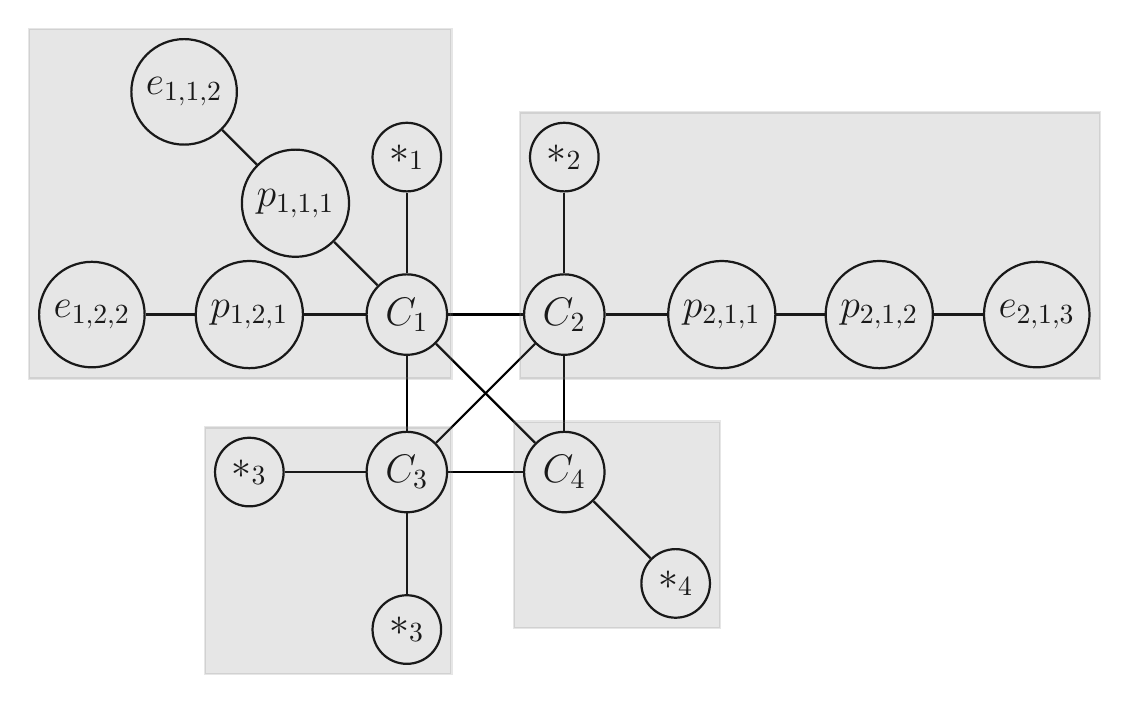
\begin{tikzpicture}[-,auto,node distance=2cm,
                    thick,main node/.style={circle,draw,font=\sffamily\Large\bfseries}]

 \node[main node] (c1) {$C_{1}$};
 \node[main node] (1) [above of=c1] {$*_{1}$};
 \node[main node] (2) [above left of=c1] {$p_{1,1,1}$};
 \node[main node] (3) [left of=c1] {$p_{1,2,1}$};
 \node[main node] (4) [above left of=2] {$e_{1,1,2}$};
 \node[main node] (5) [left of=3] {$e_{1,2,2}$};
  
 \path
 (c1) edge (1)
      edge (2)
      edge (3)
  (2) edge (4)
  (3) edge (5);
 
 \node[main node] (c2) [right of=c1] {$C_{2}$};
 \node[main node] (6) [above of=c2] {$*_{2}$};
 \node[main node] (7) [right of=c2] {$p_{2,1,1}$};
 \node[main node] (8) [right of=7] {$p_{2,1,2}$};
 \node[main node] (9) [right of=8] {$e_{2,1,3}$};
 
  \path
 (c2) edge (6)
      edge (7)
  (7) edge (8)
  (8) edge (9);
      
 \node[main node] (c3) [below of=c1] {$C_{3}$};
 \node[main node] (10) [below of=c3] {$*_{3}$};
 \node[main node] (11) [left of=c3] {$*_{3}$};
 
  \path
 (c3) edge (10)
      edge (11);
      
 \node[main node] (c4) [below of=c2] {$C_{4}$};
 \node[main node] (12) [below right of=c4] {$*_{4}$};
 
  \path
 (c4) edge (12);            
  
 \path
 (c1) edge (c2)
      edge (c3)
      edge (c4)
 (c2) edge (c3)
      edge (c4)
 (c3) edge (c4);  
 
   \node (Box1) [draw,thick,fit=(1) (2) (3) (4) (5),fill,gray,opacity=0.2] {};
   
      \node (Box2) [draw,thick,fit=(6) (7) (8) (9),fill,gray,opacity=0.2] {};
      
         \node (Box3) [draw,thick,fit=(10) (11),fill,gray,opacity=0.2] {};
         
            \node (Box4) [draw,thick,fit=(c4) (12),fill,gray,opacity=0.2] {};
        
  
\end{tikzpicture}
\end{center}
\caption{Example of decomposition on $(S_{3}^{1,1},S_{2}^{2},S_{2},S_{1})$.}
\label{myfigure: Example of decomposition on multi general star graph}
\end{myfigure}


\begin{myfigure}
\begin{center}
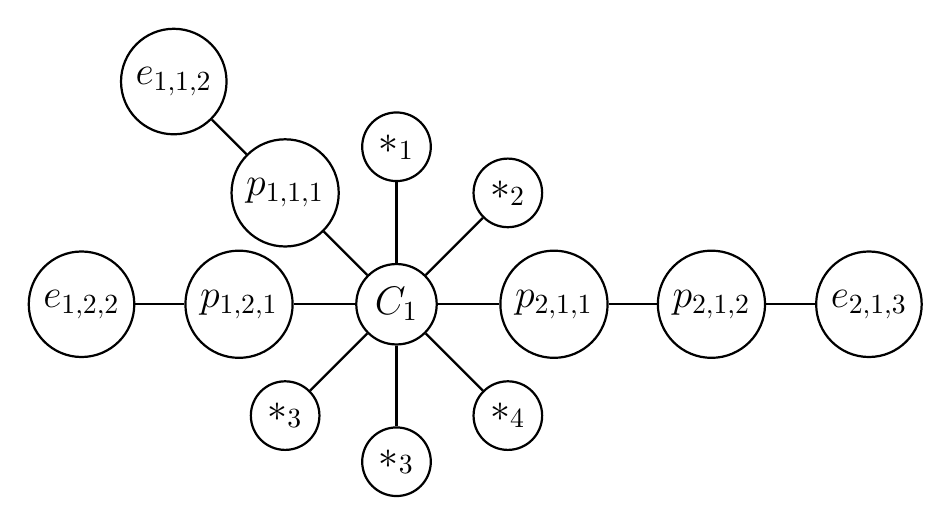
\begin{tikzpicture}[-,auto,node distance=2cm,
                    thick,main node/.style={circle,draw,font=\sffamily\Large\bfseries}]

 \node[main node] (c1) {$C_{1}$};
 \node[main node] (1) [above of=c1] {$*_{1}$};
 \node[main node] (2) [above left of=c1] {$p_{1,1,1}$};
 \node[main node] (3) [left of=c1] {$p_{1,2,1}$};
 \node[main node] (4) [above left of=2] {$e_{1,1,2}$};
 \node[main node] (5) [left of=3] {$e_{1,2,2}$};
  
 \path
 (c1) edge (1)
      edge (2)
      edge (3)
  (2) edge (4)
  (3) edge (5);
 
 \node[main node] (6) [above right of=c1] {$*_{2}$};
 \node[main node] (7) [right of=c1] {$p_{2,1,1}$};
 \node[main node] (8) [right of=7] {$p_{2,1,2}$};
 \node[main node] (9) [right of=8] {$e_{2,1,3}$};
 
  \path
 (c1) edge (6)
      edge (7)
  (7) edge (8)
  (8) edge (9);
      
 \node[main node] (10) [below of=c1] {$*_{3}$};
 \node[main node] (11) [below left of=c1] {$*_{3}$};
 
  \path
 (c1) edge (10)
      edge (11);
      
 \node[main node] (12) [below right of=c1] {$*_{4}$};
 
  \path
 (c1) edge (12);            
 
  
\end{tikzpicture}
\end{center}
\caption{Example of simplification on $(S_{3}^{1,1},S_{2}^{2},S_{2},S_{1})$ to $S_{8}^{2,1,1}$.}
\label{myfigure: Example of simplification on multi general star graph}
\end{myfigure}

\begin{note}
We note that this is not the Hamiltonian bound for such a graph and the Hamiltonian bound would be,
$$V=\frac{m}{2(|\bm{n}|+|\bm{K}|) + p}$$
\end{note}

\begin{note}
The idea of requiring the complete graph of connection between centres is not needed for the separable solution.
\end{note}

\appendix


\section{Examples}
\subsection{Example of decomposition}
\label{Appendix:Example of deocmposition}
\begin{example}
For $Q$ as seen in Figure \ref{Figure:Q decompisition example}. Consider when $m=3$, the decomposition of $Q$ into the graphs $Q_{1} \equiv L_{2}$ and $Q_{2} \equiv L_{3}$. $V_{1}=V(L_{2})=1$ as alternating between $1$ and $2$ can catch every attack. $V_{2}=V(L_{3})=\frac{3}{4}$ (as seen in \cite{Alpern2011}). 

Then we can get the bound $V \geq \frac{1}{\frac{1}{V_{1}}+\frac{1}{V_{2}}} = \frac{1}{\frac{1}{1}+\frac{3}{4}}=\frac{4}{7}$.
\end{example}

\begin{myfigure}
\begin{center}
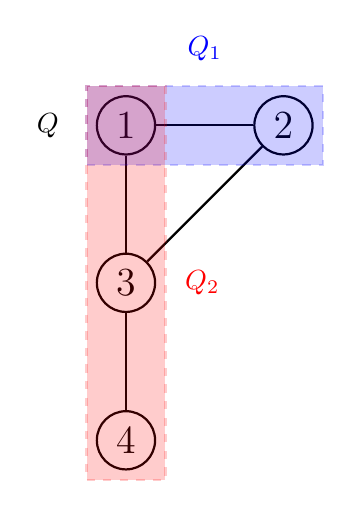
\begin{tikzpicture}[baseline=(current bounding box.north),-,auto,node distance=2cm,
                    thick,main node/.style={circle,draw,font=\sffamily\Large\bfseries}]

  \node[main node] (1) {$1$};
  \node[main node] (2) [right of=1] {$2$};
  \node[main node] (3) [below of=1] {$3$};
  \node[main node] (4) [below of=3] {$4$};

  \path[every node/.style={font=\sffamily}]
    (1) edge  (2)
    edge (3)
    (2) edge (3)
    (3) edge (4);
  
  \node (Box1) [draw=blue,dashed,thick,fit=(1) (2),fill=blue,opacity=0.2] {};  
  \node (Box2) [draw=red,dashed,thick,fit=(1) (3) (4),fill=red,opacity=0.2] {};
  
  \node [yshift=3.0ex, blue] at (Box1.north) {$Q_{1}$};
  \node [xshift=3.0ex, red] at (Box2.east) {$Q_{2}$};  
\node [left=0.5cm,text width=0.5cm] at (1)
{
$Q$
};   
\end{tikzpicture}
\end{center}
\caption{Decomposition of Q into \textcolor{blue}{$Q_{1}$} and \textcolor{red}{$Q_{2}$}.}
\label{Figure:Q decompisition example}
\end{myfigure}

\subsection{Example of simplification}
\label{Appendix:Example of simplification}
\begin{example}
For $Q$ as seen in Figure \ref{Figure:Q simplification example}, when $m=3$, the simplification of the graph by identifying nodes $1$ and $2$ simplifies $Q$ to $Q'=L_{3}$. Hence we can get the bound that $V(L_{3}) \geq  V(Q)$ so $V(Q) \leq \frac{3}{4} $.
\end{example}

\begin{myfigure}
\begin{center}
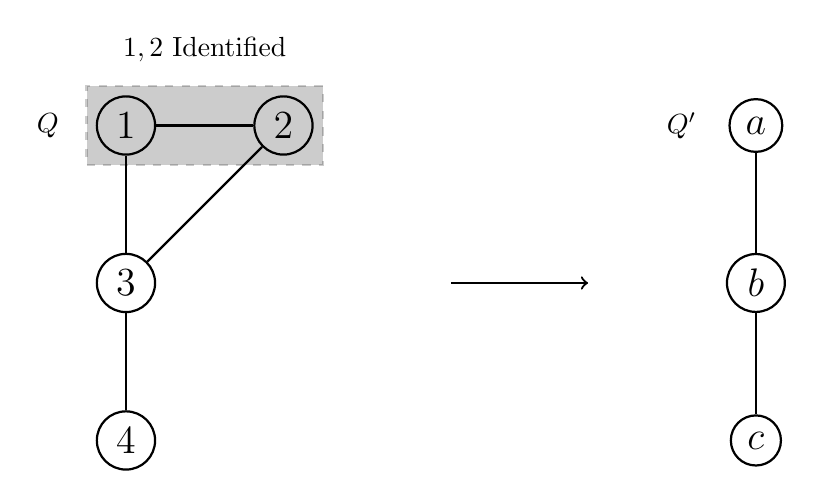
\begin{tikzpicture}[baseline=(current bounding box.north),-,auto,node distance=2cm,
                    thick,main node/.style={circle,draw,font=\sffamily\Large\bfseries}]

  \node[main node] (1) {$1$};
  \node[main node] (2) [right of=1] {$2$};
  \node[main node] (3) [below of=1] {$3$};
  \node[main node] (4) [below of=3] {$4$};
  
  \node (P1) [below of=2] {};
  \node (P2) [right of=P1] {};
  \node (P3) [right of=P2] {};
  
  \draw[->] (P2) edge (P3);
  
  \node[main node] (b) [right of=P3] {$b$};
  \node[main node] (a) [above of=b] {$a$};
  \node[main node] (c) [below of=b] {$c$};

  \path[every node/.style={font=\sffamily}]
    (1) edge  (2)
    edge (3)
    (2) edge (3)
    (3) edge (4)
    (a) edge (b)
    (b) edge (c);
  
  \node (Box1) [draw,dashed,thick,fit=(1) (2),fill,opacity=0.2] {};  
  
  \node [yshift=3.0ex] at (Box1.north) {$1,2$ Identified};  
\node [left=0.5cm,text width=0.5cm] at (1) {$Q$};
\node [left=0.5cm,text width=0.5cm] at (a) {$Q'$};   
\end{tikzpicture}
\end{center}
\caption{Simplifcation of $Q$ to $Q'$ by identification.}
\label{Figure:Q simplification example}
\end{myfigure}

\section{Patrolling games}
\subsection{Proof of diametric waiting time}
\label{Appendix:Proof of diametric waiting time}

Consider visit $i$ to a end node capturing $C_{i}$ of the attacks placed by the diametric attack, then the total number of attacks captured is $C=\sum\limits_{i=0}^{\floor{\frac{T-1}{\bar{d}}}} C_{i}$.

Then leaving the initial node at time $t$ gives us, $C_{0}=\min(t,T-m+1)$ , $C_{i}=\pospart{\min(t+i \bar{d},m,T-(t+i \bar{d})}$ for $i \neq 0$.

We first note that $C_{0}$ is increasing in the region $t \leq T-m$ and constant for $t \geq T-m+1$. So $C_{0}$ is concave. Due to this being increasing, and therefore its only possible to have others increasing if $t \leq T-m$, we will make this an assumption.

Now we look at $C_{i}$ and see it is increasing for the region $t \leq m-1-i\bar{d}$, constant for $m-i\bar{d} \leq t \leq T-1-m-i \bar{d}$ and decreasing for $ T-m-i \bar{d} \leq t \leq T-i \bar{d}-1$. So $C_{i}$ is concave. Hence $C$ is concave and so finding the best choice for $t$ is when the net increase is constant (or decreasing for the first time).

We see that $C_{0}$ always improves, contributing $1$ to the net increase. $C_{i}$ however is only increasing, and contributes $1$, if $i \leq \frac{m-1-t}{\bar{d}} < 2$ (as $m \leq 2\bar{d}$), so only $C_{1}$ can possibly contribute an increase when $t \leq m-\bar{d}-1$.

$C_{i}$ is decreasing, contributing $-1$ if $\frac{T-m-t}{\bar{d}} \leq i \leq \frac{T-1-t}{\bar{d}}$, with at most $2$ $C_{i}$'s being decreased (as the gap is $\frac{m}{2 \bar{d}}$ and $\bar{d} < m \leq 2 \bar{d}$).

This worst issue occurs when $\frac{T-m-t}{\bar{d}}$ or $\frac{T-1-t}{\bar{d}}$ are integers, meaning we have chosen $t=T-m-k\bar{d}$ or $t=T-1-k\bar{d}$ for some $k \in \mathbb{Z}$.

So overall increasing $t$ to $t+1$, with $t \leq m-\bar{d}-1$, gives us a net increase of $1$ when we have non-integers, $0$ when we have integers  and $-1$ if $t > m- \bar{d}-1$.

So we pick the upper concave region, as its about to go from increasing to decreasing, giving us a choice of $t=m-\bar{d}$.
 
Note. $t=m-\bar{d}-1$ is not net decreasing, but $t=m-\bar{d}-1$ is net decreasing, so $t=m-\bar{d}$ is a choice for the maximum.

\subsection{Proof of conditions on T for diametric attack}
\label{Appendix:Proof of conditions on T for diametric attack}

We first justify the counting formula,

\begin{align*}
&\underbrace{m-\bar{d}}_{\text{Waiting initially}} + \underbrace{\pospart{m \times \left( M +1 \right)}}_{\text{Visits which get exactly } m \text{ attacks}} \\
&+ \underbrace{\pospart{T- \left( m-1 + \left(M +1 \right) \bar{d} \right)}+\pospart{T- \left( m-1 + \left(M +2 \right) \bar{d} \right)}}_{\text{Penultimate and final node visits}} 
\end{align*}

Where $M=\floor{\frac{T-2m+1}{\bar{d}}}$.

Initially by waiting till time $m-\bar{d}-1$ the patroller collect $m-\bar{d}$ potential attacks, they then leave and hit the next diametric node at time $m-1$ getting them $m$ potential attacks.

Then we notice that the last time we can arrive at diametric node to get $m$ potential attacks is at time $T-m$. so how many diametric nodes do we get exactly $m$ at , the initial one (at time $m-1$) and then $\floor{\frac{T-m-(m-1)}{\bar{d}}} = \floor{\frac{T-2m+1}{\bar{d}}}=M$ additional ones. This is the second piece of the equation.

For the final piece we consider the times we are a diametric node, after we get $m$, we will be there at times $m-1+(M+1)\bar{d} , m-1+(M+2)\bar{d}, ...$, getting us $T-m+1-(M+1)\bar{d},T-m+1-(M+2)\bar{d},...$. As we know that $T-m+1-(M+1)\bar{d} < m \implies T-m+1-(M+3)\bar{d},T-m+1-(M+4),...<0$, so we only have possibly the penultimate and final node visits.

Hence the result is as above.

\begin{proof}
Using $T=m-1+(k+1)\bar{d}$ in the formula gives,
$M=\floor{\frac{(k+1) \bar{d}-m}{\bar{d}}}=(k+1)+\floor{\frac{-m}{\bar{d}}}=(k+1)-2=(k-1)$ (the final part is because $2>\frac{-m}{\bar{d}} \geq -1$ and we will assume that $m > \bar{d}$ here otherwise waiting at one node is just as good as the bound we are trying to achieve).

$m-\bar{d}+\pospart{m + m(k-1)} + \pospart{m-1-(m-1+(k-1+1)\bar{d})}+\pospart{m-1-(m-1+(k+1)\bar{d})}$

which is $m-\bar{d}+\pospart{mk} + \pospart{(k+1)\bar{d}-k\bar{d}}+\pospart{(k+1)\bar{d}-(k+1)\bar{d}}$
giving $m-\bar{d}+mk+ \pospart{\bar{d}}+\pospart{0}=m(k+1)$.
Giving the fraction of $\frac{m(k+1)}{2(k+1)\bar{d}}=\frac{m}{2 \bar{d}}$.


For the second part, first we seek to prove that within the choice of $T$ from $m-1+(k+1)\bar{d}+r$ where $0 \leq r < \bar{d}$ is the maximum when $r=m-\bar{d}$ (i.e $T=2m-1+k\bar{d}$).

As the choice of $r$ only affects the final 3 parts (middle and ends values), we can just look at considering these values and seeing what the maximal choice is.

Upon substitution we get that:
$M=\floor{\frac{(k+1)\bar{d}+r-m}{\bar{d}}}=(k+1)+\floor{\frac{r-m}{\bar{d}}}$

Then we notice two cases:

\begin{itemize}
\item[1.] If $0 \leq r < m-\bar{d}$ then $M=k-1$ and we get a fraction of potential attacks caught of $\frac{m(k+1)+2r}{2((k+1)\bar{d}+r)}$

\item[2.] If $m-\bar{d} \leq r < \bar{d}$ then $M=k$ and we get a fraction of potential attacks caught of $\frac{m(k+1)+r+m-\bar{d}}{2((k+1)\bar{d}+r)}$ 
\end{itemize}

Hence the best in the first case is $r=m-\bar{d}-1$ for $\frac{m(k+3)-2\bar{d}-2}{2(k\bar{d}+m-1)}$ and in the second case $r=m-\bar{d}$ for $\frac{m(k+3)-2\bar{d}}{2(k\bar{d}+m)}$, hence it is clear the best is $r=m-\bar{d}$.

Then we show that the maximal subsequence tends to the bound as $T \rightarrow \infty$, i.e as $k \rightarrow \infty$. Well the maximal subsequence is $\frac{m(k+3)-2 \bar{d}}{2(k \bar{d}+m)} \rightarrow \frac{m}{2 \bar{d}}$ as $k \rightarrow \infty$, hence as the maximal subsequence tends down to the bound, it implies the result stated.
\end{proof}

\subsection{Proof of time-limited diametric attack}
\label{Appendix:Proof of time-limited diametric attack}

\begin{proof}
First consider all the pure patrolling strategies, $W_{i} \in \mathcal{W}$, Then as the attacker is only attacking two ends, henceforth called $n_{1}$ and $n_{\bar{d}}$, any patrol not starting at $n_{1}$ or $n_{\bar{d}}$ is dominated by one that does.
This is because the patrol will not capture any attacks until they visit either $n_{1}$ or $n_{\bar{d}}$, and then capture a set of attacks that started there previously. The patrol might as well wait there up until this point and do at least as good as arriving there for the first time.

Formally, assume that $n_{1}$ is the end node first reached by a patrol, $W(t)$ at time, $t_{1}=\min \set{t}{W(t)=n_{1}}$, then we can form the patrol, $U(t)= \left\{ \begin{array}{l}
n_{1} \text{ for } t \leq t_{1}, \\
W(t) \text{ for } t>t_{1}. \\
\end{array} \right.$
and $P(U,\phi) \geq P(W,\phi)$ where $\phi$ is the timed diametric attack (or infact the normal diametric attack.

Now we are restricted to patrols starting at end points, it is similar to see when leaving an end point, there is no other decision as you must travel to the other end point, assumed to be $n_{\bar{d}}$. Hence the question becomes when to leave $n_{1}$ and travel to $n_{\bar{d}}$. Obviously it should only be undertaken if the journey can be made and more attacks can be caught by doing so.

WLOG assume that $\tau=0$ (other just wait longer initially, as attacks haven't started), then our choice is what leaving time (last time before moving): $t_{l} \in \{0,1,...,m-2 \}$, to pick to maximize the number of attacks caught; or $t_{L}=\infty$, never leaving to get $\bar{d}$ attacks.

\begin{itemize}
\item[Leaving:]Choosing $t_{L} \in \{0,1,...,m-2 \}$ gives the patroller $\frac{m}{2\bar{d}}$ as,

Leaving at $t_{L}$ gives us $\min(t_{L}+1,\bar{d})$ attacks caught at $n_{L}$, and $\min(m+\bar{d}-2-(t_{L}+\bar{d})+1,\bar{d})=\min(m-1-t_{L},\bar{d})$.

Now choosing $t_{L} > \bar{d}-1$, doesn't improve the first value and possibly lowers the second value. Hence we restrict ourselves to leave if we catch all attacks, i.e $t_{L} \leq \bar{d}-1$. Now in this region lowering $t_{L}$ lowers it by $1$ and raises it only raises the second on by $1$ if $m-1-t_{L} \leq \bar{d}$ (i.e $t_{L} \geq m-1-\bar{d}$ or any $t_{L}$ if $m-1-\bar{d} \leq 0$). Hence any choice of $\pospart{m-1-\bar{d}} \leq t_{L} \leq \bar{d}-1$ is equally as good. This gives a number of attacks caught as $t_{L}+1+m-1-t_{L}=m$ out of $2\bar{d}$ placed attacks. Hence giving $V \leq \frac{m}{2\bar{d}}$.

\item[Staying:]Choosing $t_{L}=\infty$ gives the patroller $\frac{1}{2}$
\end{itemize}

Hence as the patroller can pick from these two options, it gives $V \leq \max\{\frac{1}{2} , \frac{m}{2\bar{d}} \}$. More explicity it gives $V \leq \frac{1}{2}$ if $m < \bar{d}$, and $V \leq \frac{m}{2\bar{d}}$ is $m \geq \bar{d}$.
\end{proof}

\subsection{Proof of time-delayed attack}
\label{Appendix:Proof of time-delayed attack}

\begin{proof}
First Consider a patrolling strategy that is at a $*$ node at time $t \geq k$ (i.e $*$ node attacks have begun) and seek to show that staying amongst the $*$ nodes until the attacks end is at least as good as moving to node $1$ and waiting, and possibly returning to $*$ (if time allows).

We will consider two cases of $m \leq 2(k+1)$ and $m > 2(k+1)$.
\begin{itemize}
\item[1.] In this case we will first show that returning to $*$ type nodes is never an option once it is left, consider leaving at $t$, then the first possible return would be $t+2(k+2) \geq k + 2(k+2) > k+m$ and hence all the attacks would be caught and there would be no point returning. Hence the only option in this scenario is whether it is worth it leave at this point $t$ and go to node $1$ and wait until the end of the game.

If she was to stay around the end nodes then from this point onwards (not including the node we are at , at time $t$) we would get a payoff of $\frac{k+m-t-1}{2(n+k)}$.

This is becuase we either get:
\begin{itemize}
\item[$k+m$ odd] $\underbrace{\frac{1}{n+k}+...+\frac{1}{n+k}}_{\frac{k+m-t}{2} \text{times}}$
\item[$k+m$ even] $\underbrace{\frac{1}{n+k}+...+\frac{1}{n+k}}_{\frac{k+m-1-t}{2}-1 \text{times}} +\frac{1}{2(n+k)}$
\end{itemize}

In either case the payoff for moving about at the $*$ type nodes is as above.

Now consider moving away to $1$, which will be reached at time $t+k+2$ and as we must wait here the payoff depends on a few things. It is 
$$\frac{\min (m,t+k+2,m-(t+k+2-(2k+1))}{2(k+1)} \times \frac{k+1}{n+k} =
\frac{\min (m,t+k+2,k+m-t-1)}{2(n+k)}$$

now note as $t \geq k \implies m > k+m-t-1$ and as $m \leq 2(k+1) \implies t+k+2 \geq m$. Moreover this implies we will be in the final stretch of attacks and no new attacks will be taking place, so no more attacks will be claimed by waiting here (though moving back is just as fruitless).

Hence in this case the payoff is $\frac{k+m-t-1}{2(n+k)}$. The exact same benefit as to staying around the $*$ nodes, hence both moving and staying are equally as good, so once left a $*$ node she will have to wait at $1$ (and in fact the game will be over) and we have no incentive not to do it (IN FACT IF THE CONDITION ABOUT LIMITED number of $*$ nodes is brought up it is in fact the best option).

Hence for any $t \geq k$ when we are at a $*$ node we might as well move to $1$ and end the game.


Now consider being at $*$ for some time $s \leq k-1$, then we can decide to wait to time $k$ and then make the decision as above and move to $1$ or we can move immediately to $1$.

Waiting to time $k$ gives us $\frac{1}{2(n+k)} + \frac{k+m-k-1}{2(n+k)}=\frac{m}{2(n+k)}$.

Now leaving at time $s$ means we arrive at $1$ at time $s+k+2$ , however, if this is the plan then it is clear that starting at $1$ is optimal (which we will deal with next).

Now starting at $1$ at time $0$, consider the decision to move to $1$ at time $q$ (under which the decision will complete the game, as moving get us there at time $q+k+2 \geq k$ so the decision to move back immediately is chosen), This means we get a payoff of

$$ \frac{q+1}{2(n+k)} +\frac{1}{n+k} + \frac{m-(q+2(k+2)-(2k+1))}{2(n+k)}
=\frac{q+1}{2(n+k)}+\frac{1}{n+k}+\frac{m-q-3}{2(n+k)}=\frac{m}{2(n+k)} $$

With the knowledge that the choice of $q$'s choice to achieve this, if $q \geq m-2$ is chosen it is worse than the sum as, not as good on arriving and nothing gained on coming back, hence it only achieves $\frac{q+1}{2(n+k)}$, so $q=2k+1$ might as well be chosen for $\frac{k+1}{n+k}$ (note. here that $q=2k+1$ is always in this zone as $m \leq 2(k+1)$)

Hence it is best to wait for all time at node $1$ and achieve $\frac{k+1}{n+k} \geq \frac{m}{2(n+k)}$ (for $m \leq 2(k+1)$)

\item[2.] When $m > 2(k+1)$, we shall again first consider starting at a $*$ at time $t \geq k$, however now it is not possible to state that once it is left that it can never be returned to.
We care about what to do between $t$ and $k+m$, now we will first seek to show that moving and waiting at $1$ is just as good as moving around $*$ types.

Moving purely around $*$ nodes will get us as before $\frac{k+m-t-1}{2(n+k)}$.
Moving and waiting at $1$ gets us $\frac{2(k+1)-(t-m+k+1)_{+}}{2(k+1)} \times \frac{k+1}{n+k}=\frac{k+m-t-1}{2(n+k)}$. (or $\frac{2(k+1)}{2(n+k)}=\frac{k+1}{n+k}$ , if they go early enough to catch all attacks).

The only idea that could possibly be better is to move to $1$ and then wait for period of time, say $q$ times waiting, and then move back. This would yield.

$$\frac{q+ \min(2(k+1),t+k+2,t+k+2-(t-m+k+1))}{2(k+1)} \times \frac{k+1}{n+k} =\frac{q+2(k+1)}{2(n+k)} $$ ($+\frac{1}{n+k}$ or $+\frac{1}{2(n+k)}$ if arriving before all attacks at $*$ have completed) from being there for a period and then remake the decision of what to do from $t+q+2(k+2)$. During this time period between $t$ and $t+q+2(k+2)$ (assuming the game at $*$ is not over yet) then we will get

$$\underbrace{\frac{1}{n+k}+...+\frac{1}{n+k}}_{\frac{q+2k+2}{2} \text{times}}=\frac{q+2k+2}{2(n+k)}$$ ($+\frac{1}{n+k}$ or $+\frac{1}{2(n+k)}$
at end)

Hence it is better to move and wait at $1$ then return if we want to, however returning serves no purpose as we will leave immediately. Hence moving to $1$ and waiting is the best option if $t \geq k$. Hence consider starting at a $*$, it would be either wait till $k$ and move back or move earlier. Moving earlier would mean that she might as well have started at node $1$.

Hence the only option for starting at node $*$ is to get $\frac{1}{2(n+k)}+\frac{k+m-t-1}{2(n+k)}$ (or $\frac{1}{2(n+k)}+\frac{k+1}{n+k}$ if all attacks are caught at node $1$ at time $2k+2$ (i.e $m > 2k+3$)).

So starting at $*$ means getting $\frac{k+1}{n+k}+\frac{1}{2(n+k)}$ 

\end{itemize}


Let $m=2(k+1)+r$ for $r \in \mathbb{N}$.
Then considering starting at $*$ nodes, then we must decide to move to $1$ or wait till $k$ then make a decision. However deciding to move to $1$ , means we might as well have started at $1$.

If we are at a $*$ node at some time $t \geq k$ (let $t=k+t_{e}$), then we can decide to (wait only if $t=k$ until $t=k+1$) move to another $*$ node arriving at $t+2$ or move to $1$ arriving at $t+k+2$. Now we aim to show that the option of moving to another $*$ node is not strictly better. Assume it is then it is a repeated action until time $k+m-2=3k+r$ or $k+m-1=3k+r+1$ (depending on which parity we are in).

We will get a payoff of $\frac{3k+r-t}{2(n+k)}=\frac{k+m-2-t}{2(n+k)}$ or $\frac{3k+r+1-t}{2(n+k)}=\frac{k+m-1-t}{2(n+k)}$ (depending on parity). Then it will have to move to node $1$ arriving at $2k+2+m$ (and the game will be over).

Now consider moving to $1$ and waiting , arrive at time $t+k+2=2k+2+t_{e}$. Then the payoff is $\frac{\min(2(k+1),k+m-t-1)}{2(n+k)}$. Which of these is chosen as the minimum will be decided by whether they still arrive in time to collect the first few attacks (i.e it depends on the second part $k+m-t-1=2k+r-t_{e}+1$ which means if its greater than $2k+2$ i.e depending on the distant between $r-1-t_{e}$).

More explicitly the term $k+m-t-1 \geq 2k+2$ if $r-1-t_{e} \geq 0$, in this case however it is possible to make up the difference of $r-1-t-{e}$ by only waiting till $2k+1$ (we will be there at $t+k+2 \geq 2(k+1)$, so will leave immediately back) then returning to the $*$ at $3k+4$. This is in comparison to $k+m=3k+2+r$ meaning that we get an additional payoff depending on $r$'s parity.
If $r$ is odd then we gain $\frac{1}{2(n+k)}+\frac{r-2}{2(n+k)}=\frac{r-1}{2(n+k)}$.
If $r$ is even then we gain $\frac{r-1}{2(n+k)}$.

So we will be on $\frac{2(k+1)+r-1}{2(n+k)}=\frac{m-1}{2(n+k)}$ which is better than $\frac{k+m-1-t}{2(n+k)}$ and hence moving to $1$ and moving back at $2k+2$ (arriving back at $3k+4$) is better.

Similarly in the case of $2k+2> k+m-t-1$ if $r-1-t_{e} < 0$, then we can still do better by moving off, as we hit here at time $2k+2+t_{e}$ (so all attacks that are catchable have been caught), so leave and get back to star at $*$ nodes at $3k+4+t_{e}$ in comparison to $k+m=3k+2+r$ means an additional payoff depending on $r$'s parity with $t_{e}$.
In either case we get $\frac{r-t_{e}-1}{2(n+k)}$. But as this is negative it really means that all the attacks have already ended here, as $*$ attacks end at $k+m=3k+2+r$ and as we arrive at $3k+4+t_{e}$ (and $r-1-t_{e} < 0$). 
Hence no additional values can be given and an overall value of $\frac{k+m-t-1}{2(n+k)}$ is given for this case.

But in both given scenarios it is still better than waiting and playing round all the  $*$'s to end the game.

Hence it is at least as good to follow this strategy rather than repeatedly move between $*$ nodes. This means it is better than a single choice and therefore is the best thing to do in such a position.

Meaning the only option for starting at a $*$ node is to wait until $t=k$, the first real decision and decided to move to $1$ getting a payoff of either
$\frac{1}{2(n+k)}+\frac{m-1}{2(n+k)}=\frac{m}{2(n+k)}$.


If we start at $1$, then we can choose when to leave and visit $*$, say leave at time $q$ and arrive at $*$ at $q+k+2 \geq k$ as we know that from this position she will move back immediately (arriving back at $q+2(k+2)$ and hence will only get one of the nodes value of $\frac{1}{n+k}$ , once back at $1$ we will travel back to $*$, as all attacks here are over (arriving at $q+3(k+2)$). This type of strategy will get her a payoff of
$$\frac{q+1}{2(k+1)} \times \frac{k+1}{n+k} +\frac{1}{k+1} +\frac{2(k+1)-(q+1)}{2(k+1)} \times \frac{k+1}{n+k} +\frac{\pospart{r-q-3}}{2(n+k)} =\frac{k+2+\pospart{r-q-3}}{n+k} $$.

The other choice is not to visit in the middle and get all the attacks at $1$, then move across, suggest $q=2k+1$, now there is an opportunity to move to capture $*$ still occuring at $k+m=3k+2+r$ when we arrive at $3k+3$. (The complete sum depends on the parity of $r$)
We will get $\frac{r}{2(n+k)}$.
Meaning the overall payoff for playing this strategy is $\frac{k+1}{n+k}+\frac{r}{2(n+k)}=\frac{m}{2(n+k)}$.

In the case of $r-q-3 \geq 0$ then we are comparing $\frac{k+r-q-1}{2(n+k)} < \frac{m}{2(n+k)}$.

In the case of $r-q-3 < 0 $ then we are comparing $\frac{k+2}{2(n+k)} < \frac{m}{2(n+k)}=\frac{2k+2+r}{2(n+k)}$.

Hence the available strategy to her if starting at $1$ is to wait until $2k+1$ and move to the $*$ nodes claiming $\frac{m}{2(n+k)}$. If starting at $*$ has to wait until $k$ then move to $1$ and then back to $*$ claiming a payoff of $\frac{m}{2(n+k)}$.

Hence the best she can do in this situation is to follow one of the strategies.  
\end{proof}

It would be `recommended' to follow the wait at $1$ until time $2k+1$ and then move as it is also optimal for all cases of $m$, whereas starting at $*$ is only valid for $m > 2(k+1)$. 

\textbf{Altered proof below:}

\begin{proof}
We shall first consider the case of $m \leq 2(k+1)$. Consider starting at a $*$ node then the options for any time $t<k$ is wait (one time period and reconsider moving then) or move to another $*$ node or move to node $1$.

Now immediately we can remove moving to another $*$ node as this is dominated by just waiting for two time periods. Now if waiting is the dominant strategy then we must continue to wait until time $k$ upon which attacks at $*$ nodes begin.

Now consider being at a $*$ node for a time $k \leq t \leq k+m$ (when attacks are commencing), then the options are to move to another $*$ node claiming some benefit (if $t<k+m-1$, otherwise there is no point in moving and in fact the game is over at this point) or moving to $1$ (arriving at $t+k+2$) and catching some attacks there hopefully (if $t < k+m-1$, otherwise there is no point in moving and in fact the game is over).

Note. The special case of $t=k$ in which she can wait for one time period will be covered later.

Now consider that if moving to another $*$ node dominates moving to $1$ then it will be done for all time (as the generated payoff is the same, for all time, apart from possibly, from time $t=k+m-2$ in which the generated payoff either way will be $\frac{1}{2(n+k)}$).

Now moving around the star nodes from time $t$ until time $k+m-1$ or $k+m$ (depending on the parity of these values i.e $t=6$ $k+m-1=10$ (even parity) or $t=7$ $k+m=11$ (odd parity)) gives us a payoff of exactly $\frac{1}{2(n+k)}$ per unit time, or more concretely
$$\frac{k+m-1-t}{2} \times \frac{1}{n+k}=\frac{k+m-1-t}{2(n+k)} $$
or
$$\frac{k+m-2-t}{2} \times \frac{1}{n+k}+\frac{1}{2(n+k)}=\frac{k+m-1-t}{2(n+k)}$$
In either case the same value is given (note. the initial payoff for being at a $*$ node at time $t$ is not counted here).

The other decision to move to $1$ and then make a decision, means arriving at $1$ at time $t+k+2 \geq 2k+2=2(k+1)$ meaning all attacks have already begun here (and in fact it is impossible to decide to move back as return to $*$ at $t+2(k+2) \geq 3k+4 > k+m$). This means that a payoff of
$$\frac{2k+m-(t+k+2)+1}{2(k+1)} \times \frac{k+1}{n+k}=\frac{k+m-1-t}{2(n+k)}.$$
Hence it is easy to see that it is not strictly dominating the alternative strategy.

For $t=k$ we can perform the additional strategy of wait one time period to gain $\frac{1}{2(n+k)}$ then we can decide to move to $1$ getting $\frac{k+m-1-(k+1)}{2(n+k)}$, getting in total $\frac{m-1}{2(n+k)}=\frac{k+m-t-1}{2(n+k)}$, the same as above.

Now for starting at $*$ if it is before $k$ then considering moving to $1$ is dominated by just starting at $1$, so the only option is to wait until $k$ and then move to $1$ (or move around $1$ nodes, but they may not be enough) giving a total payoff of $\frac{m}{2(n+k)}$.

Now consider starting at node $1$, we could consider waiting forever and getting $\frac{k+1}{2(n+k)}$, or we could consider moving to $*$ at some point in time say $q$.

Now doing the latter, will mean we arrive at $q+k+2 \geq k$ (now assuming $q+k+2 \leq k+m-1$ i.e $q \leq m-3$) then we will catch something as following the strategy for being at $*$ after time $k$.
Meaning we get
$$\frac{q+1}{2(k+1)} \times \frac{k+1}{n+k}+\frac{1}{n+k}+\frac{k+m-1-(q+k+2)}{2(n+k)}=\frac{m}{2(n+k)}$$
(or worse if we don't arrive in time to catch attacks).

As $m \leq 2(k+1)$ it is clear that the option to wait at $1$ and catch all attacks is better giving us in this case $\frac{k+1}{n+k}$.

Now for the case of $m > 2(k+1)$ , let $m=2(k+1)+r$ (where $r \geq 1$)
\end{proof}

\begin{lemma}
The payoff for being at a $*$ node at a time $k \leq t \leq k+m-1$ is
$$\frac{\pospart{k+m-t-1}}{2(n+k)}$$
As long as [Missing condition for being in the `middle of game']
\end{lemma}
Note. This payoff does not affect the initial payoff for being at $*$ at $t$, only future decisions

\begin{proof}
We will first cover $t \geq k+1$ (and later cover $t=k$ as a special case). Now the options are to go to another star arriving at $t+2$ (then remake a decision) or to move to $1$.

Let us first look at moving to $1$, then we arrive at $1$ at time $t+k+2$ (and as $t \geq k$, it means all attacks occurring at $1$ have begun) so we claim a payoff of
$$\frac{\min\{2(k+1)-x,\pospart{2k+m-(t+k+2)+1-x)}\}}{2(k+1)} \times \frac{k+1}{n+k}=\frac{\min\{2(k+1),\pospart{k+m-t-1-x}\}}{2(n+k)}$$
Where $x \geq 0$ is the overlap with attacks already caught.

Now choosing to move to $s$ $*$ nodes before moving to $1$ gives a payoff of
$$s \times \frac{1}{n+k} + \frac{\min \{2(k+1)-\pospart{x},\pospart{k+m-t-2s-1-\pospart{x-2s}} \}}{2(n+k)}$$.

So it is best to move to all the $*$ nodes, which haven't been visited before, before moving to $1$.

In the case of $m \leq 2(k+1)$, it is impossible to get any overlap as the time to leave and return is at least $2(k+2) > m$, so in this case $x=0$. Also $\pospart{k+m-t-1} \leq m-1 < 2(k+1)$, so the payoff from moving to $1$ immediately becomes
$$\frac{k+m-t-1}{2(n+k)}$$
Similarly the other case becomes
$$s \times \frac{1}{n+k} + \frac{k+m-t-1-2s}{2(n+k)}=\frac{k+m-1-t}{2(n+k)}$$

In the case of $m > 2(k+1)$ (let $m=2(k+1)+r$), overlap is definitely possible if $1$ has been visited before. Now the game ends if she is at a $*$ at any time past $k+m = 3k+2+r$ or at $1$ at any time past $2k+m = 4k+2+r$.

If $1$ hasn't been visited before then $x=0$ $\pospart{k+m-t-2s-1-\pospart{x-2s}}=\pospart{k+m-t-2s-1}=\pospart{3k+1+r-t-2s} \leq \pospart{2k+1+r-2s}$,the payoff becomes either

$$s \times \frac{1}{n+k} +\frac{k+1}{n+k}=\frac{k+s+1}{n+k}$$ if $3k+1+r-t-2s > 2k+2$ (i.e $k-1+r-t-2s > 0$, so $2s<k+r-1-t$)
\\
or
$$s \times \frac{1}{n+k} +\frac{3k+1+r-t-2s}{2(n+k)}=\frac{k+m-t-1}{2(n+k)}$$ otherwise.

Examining the first part gives us
$$\frac{k+s+1}{n+k}=\frac{2(k+1)+2s}{2(n+k)} < \frac{2(k+1)+k+r-1-t}{2(n+k)}< \frac{k+m-1-t}{2(n+k)}$$.
We will end at $1$ at time $t+2s+k+2$, meaning we might as well choose $s=0$ and arrive as early as possible getting $\frac{k+m-t-1}{2(n+k)}$.

If there is some overlap then we will get the above if $x-2s \leq 0$ (except the first part will be even worse with $-x$ in the numerator).

If $x > 2s$ though then we will get either
$$s \times \frac{1}{n+k} + \frac{2(k+1)-x}{2(n+k)}=\frac{2(k+1)+2s-x}{n+k}$$ if $3k+1+r-t-2s-(x-2s) > 2k+2$ (i.e $k+1+r-t-x > 0$ ,

$$s \times \frac{1}{n+k} + \frac{3k+1-t-2s-(x-2s)}{2(n+k)}=\frac{3k+1-t-x+2s}{2(n+k)}=\frac{k+m-1-t-x+2s}{2(n+k)} $$

Hence in this case the best we can do is pick the highest $s$ to try not to overlap as much.

In any case the best she can do from this position is $\frac{k+m-t-1}{2(n+k)}$.
\end{proof}

\begin{proof}
We will first deal with the case that $t \geq k+1$. We will also first assume that there is no initial overlap of attacks at $1$ caught, that is if we arrive at node $1$ at $t+k+2$ we will not be there at a time when attacks we previously caught would still be happening.
Let the overlap be denoted by $x$, so first look at $x=0$. Now our only choice from node $*$ is to move to $s$ other $*$ nodes that we haven't yet visited and then move to $1$ (in the hope of catching some attacks).

The payoff for doing this gives us
\begin{align*}
&s \times \frac{1}{n+k} +\frac{\min \{ 2(k+1), \pospart{2k+m-(t+2s+k+2)+1-x} \}}{2(k+1)} \times \frac{k+1}{n+k} \\
&=\frac{2s}{(n+k)} +\frac{\min \{ 2(k+1), \pospart{k+m-t-1-2s-x} \}}{2(n+k)} 
\end{align*}
and as $x=0$
\begin{align*}
\frac{2s}{2(n+k)} +\frac{\min \{ 2(k+1), \pospart{k+m-t-1-2s} \}}{2(n+k)} 
\end{align*}
From this it should be clear that the payoff is non-decreasing in $s$ and so choosing $s$ as the maximum would seem to be a logical choice.

Now for a moment we will consider the future when we are at $1$, as we will arrive at time $t+k+2+2s \geq 2k+2+2s \geq 2k+2$ all attacks occuring at $1$ have been and we should no longer consider waiting or returning to this node, also moving away brings us back to $*$ nodes (arriving at time $t+2(k+2)+2s \geq 2k+4+2s$ , when the attacks end at $k+m-1$ or $k+m$), now as before all attacks have begun but they may not have ended. Hence we could consider moving around these $*$ nodes until the game ends. This means we actually get a payoff of

\begin{align*}
&\frac{2s}{2(n+k)}+\frac{\min \{ 2(k+1), \pospart{k+m-t-1-2s} \}}{2(n+k)} +\frac{\pospart{\frac{k+m-1-(t+2(k+2)+2s)}{2}}}{n+k} \\
&=\frac{2s}{2(n+k)}+\frac{\min \{ 2(k+1), \pospart{k+m-t-1-2s} \}}{2(n+k)} +\frac{\pospart{m-k-5-t-2s}}{2(n+k)} 
\end{align*}
or
\begin{align*}
&\frac{2s}{2(n+k)}+\frac{\min \{ 2(k+1), \pospart{k+m-t-1-2s} \}}{2(n+k)} +\frac{\pospart{\frac{k+m-2-(t+2(k+2)+2s)}{2}}}{n+k}+\frac{1}{2(n+k)} \\
&=\frac{2s}{2(n+k)}+\frac{\min \{ 2(k+1), \pospart{k+m-t-1-2s} \}}{2(n+k)} +\frac{\pospart{m-k-5-t-2s}}{2(n+k)} 
\end{align*}
So we only need to worry about this is $m-k-5-t-2s >0$.
If $m=2(k+1)+r$ then $m-k-5-t-2s=2(k+1)+r-k-5-t-2s=k+r-3-t-2s$
So if $k+r-3-t-2s> 0$ then we will worry about this possibility of doing the movement at the ends.
However if $k+r-3-t-2s >0 \implies 3k+1+r-t-2s>2(k+1) \implies k+m-t-1-2s>2(k+1)$, meaning that the payoff actually becomes
\begin{align*}
\frac{2s}{2(n+k)}+\frac{2(k+1)}{2(n+k)} +\frac{m-k-5-t-2s}{2(n+k)}
=\frac{k+m-t-3}{2(n+k)}
\end{align*}
So in this case, the choice of $s$ is irrelevant.
Hence we might as well pick $s$ to be the highest possible, call it $s_{max}=\min \{ n-1-y,\frac{k+m-1-t}{2} \}$ (if odd parity) or $s_{max}=\min \{ n-1-y, \frac{k+m-t}{2} \}$ (if even parity)(Note. In even parity we will get the starting payoff slightly differently).
Where $y$ is the number of currently visited $*$ nodes at time $t$.

For each type of parity let us cover the two cases,
\begin{itemize}
\item[Odd Parity:]
\begin{itemize}
\item[1.]Let $n-1-y \geq \frac{k+m-1-t}{2}$ then the payoff we get becomes
\begin{align*}
&\frac{\frac{k+m-1-t}{2}}{n+k}+\frac{\min \{ 2(k+1),\pospart{k+m-t-2 \times \frac{k+m-1-t}{2}-1} \}}{2(n+k)} \\
&=\frac{k+m-1-t}{2(n+k)} +\frac{\min \{ 2(k+1),0 \}}{2(n+k)}
=\frac{k+m-1-t}{2(n+k)}
\end{align*}
\item[2.]Let $n-1-y < \frac{k+m-1-t}{2}$ then the payoff we get becomes
\begin{align*}
\frac{n-1-y}{n+k}+\frac{\min \{ 2(k+1),\pospart{k+m-t-2(n-1-y)-1} \}}{2(n+k)}
\end{align*}
Further split into subcases
\begin{itemize}
\item[a)]Let $k+m-t-2(n-1-y)-1<0$ then the payoff becomes
\begin{align*}
\frac{n-1-y}{n+k}<\frac{k+m-t-1}{2(n+k)}
\end{align*}
\item[b)]Let $0 \leq k+m-t-2(n-1-y)-1 \leq 2(k+1)$ then the payoff becomes
\begin{align*}
\frac{n-1-y}{n+k} +\frac{k+m-t-2(n-1-y)-1}{2(n+k)}=\frac{k+m-t-1}{2(n+k)}
\end{align*}
\item[c)]Let $k+m-t-2(n-1-y)-1 > 2(k+1)$ then the payoff becomes
\begin{align*}
&\frac{n-1-y}{n+k}+\frac{2(k+1)}{2(n+k)}
&=\frac{n+k-y}{n+k} < \frac{k+m-t-1}{2(n+k)}
\end{align*}
As $k+m-t-2(n-1-y)-1 > 2(k+1) \implies k+m-t-1 > 2(n-1-y+k+1)=2(n+k-y)$
\end{itemize}
\end{itemize}

\item[Even Parity:]
\begin{itemize}
\item[1.]Let $n-1-y \geq \frac{k+m-t}{2}$ then the payoff we get becomes
\begin{align*}
&\frac{\frac{k+m-t}{2}-1}{n+k}+ +\frac{1}{2(n+k)}+\frac{\min \{ 2(k+1),\pospart{k+m-t-2 \times \frac{k+m-t}{2} -1} \}}{2(n+k)} \\
&=\frac{k+m-1-t}{2(n+k)} +\frac{\min \{ 2(k+1),\pospart{-1} \}}{2(n+k)}
=\frac{k+m-1-t}{2(n+k)}
\end{align*}
\item[2.]Let $n-1-y < \frac{k+m-t}{2}$ then the payoff we get becomes
\begin{align*}
\frac{n-1-y}{n+k}+\frac{\min \{ 2(k+1),\pospart{k+m-t-2(n-1-y)-1} \}}{2(n+k)}
\end{align*}
Note. In this case, the `problem' with having a final time only pick up $\frac{1}{2(n+k)}$ is not possible as we will have left before this time.
Further split into subcases
\begin{itemize}
\item[a)]Let $k+m-t-2(n-1-y)-1<0$ then the payoff becomes
\begin{align*}
\frac{n-1-y}{n+k}<\frac{k+m-t-1}{2(n+k)}
\end{align*}
\item[b)]Let $0 \leq k+m-t-2(n-1-y)-1 \leq 2(k+1)$ then the payoff becomes
\begin{align*}
\frac{n-1-y}{n+k} +\frac{k+m-t-2(n-1-y)-1}{2(n+k)}=\frac{k+m-t-1}{2(n+k)}
\end{align*}
\item[c)]Let $k+m-t-2(n-1-y)-1 > 2(k+1)$ then the payoff becomes
\begin{align*}
&\frac{n-1-y}{n+k}+\frac{2(k+1)}{2(n+k)}
&=\frac{n+k-y}{n+k} < \frac{k+m-t-1}{2(n+k)}
\end{align*}
As $k+m-t-2(n-1-y)-1 > 2(k+1) \implies k+m-t-1 > 2(n-1-y+k+1)=2(n+k-y)$
\end{itemize}
\end{itemize}
\end{itemize}

Now let us consider that there is some initial overlap, being more concretely $x=x(s)=\pospart{x(0)-2s}=\pospart{x_{0}-2s}$. Then if $x-2s\ leq 0$ we get the same as above.
Otherwise if $x geq 1$ then the payoff is
\begin{align*}
&\frac{s}{n+k}+\frac{\min \{ 2(k+1),\pospart{k+m-t-1-2s-(x_{0}-2s)} \}}{2(n+k)}\\
&=\frac{s}{n+k}+\frac{\min \{ 2(k+1),\pospart{k+m-t-1-x_{0}} \}}{2(n+k)}
\end{align*}
And again the payoff is non-decreasing in s, so again $s_{max}$ is the best choice.
We can follow a similar idea to the above when there was no overlap, though has the chance of being lower. Hence it will only harm the values.

The exact algebra follows the same process except now the second term in the visiting of node $1$ has a subtraction and is therefore less rewarding. 

Hence from this position the best the patroller can do is get a payoff of $\frac{k+m-t-1}{2(n+k)}$ and the best patroller strategy is to travel amongst as many $*$ nodes that have not already been visited and then head off to $1$.

Now consider the special case of being at a $*$ at $t=k$, then the above can be followed to achieve no better than $\frac{m-1}{2(n+k)}$ or we can wait and pick up $\frac{1}{2(n+k)}$ by catching the second attack and then proceed to follow the above at $t=k+1$ getting $\frac{m-2}{2(n+k)}$. Either strategy yields the same payoff, so we shall suggest just strictly following the above.
\end{proof}

\begin{theorem}[Lower Bound]
$$V \leq \max \left\{ \frac{k+1}{n+k} , \frac{m}{2(n+k)} \right\}$$
\end{theorem}

\begin{proof}
Suppose the patroller starts at a $*$ node at time $t \leq k-1$, then the options are to move to node $1$ which is dominated by just starting at node $1$ and waiting till $t+k+2$ (as no attacks are picked up at $*$ nodes. Or she can wait till time $t$ and follow the above lemma getting a payoff of
$$\frac{1}{2(n+k)}+\frac{m-1}{2(n+k)}=\frac{m}{2(n+k)}$$. So starting at $*$ provides a payoff of at most $\frac{m}{2(n+k)}$
Now consider starting at node $1$ at time $0$ then if we leave and want to return we can only do so once (as upon the first return the time will be at least $2(k+2)$ so all attacks will have begun).

Now split the solution into two regions for $m=2(k+1)+r$, for $-2(k+1)+1 \leq r \leq 0$ and $r \geq 1$.
Consider waiting until time $q$ and then leaving, as you will hit a $*$ node at time $q+k+2$ meaning we can use the lemma to generate the max payoff here. For a total payoff of
\begin{itemize}
\item[1.] If $q+k+2 > k+m=3k+2+r$
\begin{align*}
&\frac{q+1}{2(k+1)} \times \frac{k+1}{n+k} + \frac{\pospart{k+m-(q+k+2)-1}}{2(n+k)} \\
&= \frac{q+1}{2(n+k)}  
\end{align*}
\item[2.] If $q+k+2=k+m=3k+2+r$
\begin{align*}
&\frac{q+1}{2(k+1)} \times \frac{k+1}{n+k}+\frac{1}{2(n+k)}
+\frac{\pospart{k+m-(q+k+2)-1}}{2(n+k)}\\
&= \frac{q+2}{2(n+k)}  
\end{align*}
\item[3.] If $q+k+2 \leq k+m=3k+2+r$
\begin{align*}
&\frac{q+1}{2(k+1)} \times \frac{k+1}{n+k}+\frac{1}{n+k}+\frac{\pospart{k+m-(q+k+2)-1}}{2(n+k)} \\
&= \frac{m}{2(n+k)}  
\end{align*}
\end{itemize}
So as these are non-decreasing in $q$ we pick $q=2k+1$.
Then we get 
\begin{itemize}
\item[1.] If $3k+3 > 3k+2+r$ i.e $r \leq 0$
\begin{align*}
\frac{2k+1+1}{2(n+k)}=\frac{k+1}{n+k}  
\end{align*}
\item[2.] If $3k+3=3k+2+r$ i.e $r=1$
\begin{align*}
\frac{2k+1+2}{2(n+k)}=\frac{2(k+1)+1}{2(n+k)}=\frac{m}{2(n+k)}  
\end{align*}
\item[3.] If $q+k+2 \leq k+m=3k+2+r$ i.e $r \geq 2$
\begin{align*}
\frac{m}{2(n+k)}  
\end{align*}
\end{itemize}

Hence if $m \leq 2(k+1)$ (i.e $r \leq 0$) then we get $\frac{k+1}{n+k}$ and if $m > 2(k+1)$ (i.e $r \geq 1 $) we get $\frac{m}{2(n+k)}$ and hence the result.
\end{proof}

\subsection{Proof of type-delayed attack}
\label{Appendix:Proof of type-delayed attack}
We begin with a lemma used in the proof
\begin{lemma}
When $k_{max}-i \leq t \leq k_{max}+i$ we get that
$$\frac{\pospart{k_{max}+1+i-t}}{2 \left( \denominator \right)} + \frac{\pospart{m-2(i+1)}}{2 \left( \denominator \right)} \geq \frac{\pospart{k_{max}-i+m-t-1}}{2 \left( \denominator \right)} $$
\end{lemma}

\begin{proof}
If $m \geq 2(i+1)$, then we get
$$\frac{k_{max}+1+i-t+m-2(i-1)}{2 \left( \denominator \right)}=\frac{k_{max}-i+m-t-1}{2 \left( \denominator \right)} \geq \frac{\pospart{k_{max}-i+m-t-1}}{2 \left( \denominator \right)}$$

If $m \leq 2(i+1)$, then we get
$$\frac{k_{max}+1+i-t}{2 \left( \denominator \right)} \geq \frac{\pospart{k_{max}+1+i-t+m-2(i+1)}}{2 \left( \denominator \right)} =\frac{\pospart{k_{max}-i+m-t-1}}{2 \left( \denominator \right)}$$
\end{proof}

The main proof of the attack lemma's future payoff

Note. The difference in future payoffs depends on whether the patroller has the option to wait (till the last attack at the type $i$ node) or whether they have no option but to move.

Remark. It is worth noting that the game essentially ends at time $t=2k_{max}+m$, so this is really the last time we could possibly care about. Further as a type $i$ node attacks finish at $t=k_{max}+i+m$, and so a movement to a type $j$ node means arriving at $t=k_{max}+2i+2+j+m \geq k_{max}+j+m$ $\forall \, j$, meaning that no future attacks can be caught if at a type $i$ node at $t=k_{max}+i+m$, and this means this is the artificial end for the game at a type $i$ node.

\begin{lemma}
When the Type-delayed attack is possible, then the future payoff for being at a type $i$ node at time $t$ is given by:
\begin{align*}
&\frac{\pospart{k_{max}+1+i-t}}{2 \left( \denominator \right)} + \frac{\pospart{m-2(i+1)}}{2 \left( \denominator \right)} \text{  if } k_{max}-i \leq t \leq k_{max}+i \\
&\frac{\pospart{k_{max}-i+m-t-1}}{2 \left( \denominator \right)} \text{  if } t \geq k_{max}+i+1
\end{align*}
\end{lemma}

\begin{proof}
We will first prove the statement for when $t \geq k_{max}+i+1$, by the use of strong backwards induction.

\textbf{Base Case:}
\\
For $t=k_{max}+i+m$, as above it is known that no future attacks can be caught (and the game is over) as arriving at a type $j$ means arriving at $k_{max}+2i+j+2+m \geq k_{max}+j+m$ meaning all attacks are over ($\forall \, j$). Hence the future payoff is $0$.
Now the formula gives $$\frac{\pospart{k_{max}-i+m-(k_{max}+i+m)-1}}{2 \left( \denominator \right)}=\frac{\pospart{-2i-1}}{2 \left( \denominator \right)}=0$$
Hence it is true for $t=k_{max}+i+m$.

\textbf{Induction hypothesis:}
\\
For some $t_{1} \geq k_{max}+i+1$ assume that the formula for $t \geq k_{max}+i+1$ is true for all $t \geq t_{1} +1$.

\textbf{Induction step:}
\\
At a type $i$ node at time $t_{1} \geq k_{max}+i+1$, all attacks have begun at this node so waiting is not really an option (i.e it is clearly dominated by moving immediately). So moving to a type $j$ means arriving at $t_{1}+i+2+j$ giving an immediate payoff and meaning (under the Induction hypothesis) a future payoff is received. Giving at best a total payoff of
\begin{align*}
&\underbrace{\frac{\min (2(j+1), \pospart{k_{max}+j+m-(t_{1}+i+2+j)+1})}{2(j+1)} \times \frac{j+1}{\denominator}}_{\text{Immediate reward at type } j} \\
&+\underbrace{\frac{\pospart{k_{max}-j+m-(t_{1}+i+2+j)-1}}{2 \left( \denominator \right)}}_{\text{Future reward from type } j} \\
&=\frac{\min (2(j+1), \pospart{k_{max}+m-t_{1}-i-1})}{2 \left( \denominator \right)}
+\frac{\pospart{k_{max}-i+m-t_{1}-2j-3}}{2 \left( \denominator \right)}
\end{align*}
Now we will split it into the subcase of $2(j+1) \geq k_{max}+m-t_{1}-i-1$. This means $k_{max}+m-t_{1}-3-2j \leq 0$, then the payoff becomes
\begin{align*}
\frac{\pospart{k_{max}+m-t_{1}-i-1})}{2 \left( \denominator \right)}
\end{align*}
Otherwise if $2(j+1) < k_{max}+m-t_{1}-i-1$. This means $k_{max}+m-t_{1}-i-3-2j > 0$, then the payoff becomes
\begin{align*}
&\frac{2(j+1)+k_{max}-i+m-t_{1}-2j-3}{2 \left( \denominator \right)}=\frac{k_{max}-i+m-t_{1}-1}{2 \left( \denominator \right)} \\
&=\frac{\pospart{k_{max}-i+m-t_{1}-1}}{2 \left( \denominator \right)}
\end{align*}

Hence by mathematical induction it is true for $t \geq k_{max}+i+1$ and the form is correct.

Next we seek to prove the formula for the values of $t \leq k_{max}+i$, again using strong backwards induction.

\textbf{Base case:}
\\
For $t=k_{max}+i$, we have the option to wait for one unit of time (to catch the final attack at this node) and then claim the reward for this and the future rewards, or can move immediately to some type $j$ node (arriving at $k_{max}+2i+2+j$ and claim the reward and future rewards.

Waiting gives
\begin{align*}
&\frac{1}{2(i+1)} \times \frac{i+1}{\denominator} +\frac{\pospart{k_{max}-i+m-(k_{max}+i+1)-1}}{2 \left( \denominator \right)} \\
&=\frac{1}{2 \left( \denominator \right)}+\frac{\pospart{m-2(i+1)}}{2 \left( \denominator \right)}
\end{align*}
Moving gives
\begin{align*}
&\frac{\min (2(j+1), \pospart{k_{max}+j+m-(k_{max}+2i+2+j)+1})}{2 \left( \denominator \right)} \\
&+\frac{\pospart{k_{max}-j+m-(k_{max}+2i+2+j)-1}}{2 \left( \denominator \right)} \\
&=\frac{\min (2(j+1),\pospart{m-2i-1})+\pospart{m-2i-2j-3}}{2 \left( \denominator \right)}
\end{align*}
When moving it will depend on if $2(j+1) \geq m-2i-1$, which means $m-2i-2j-3 \leq 0$
giving $\frac{\pospart{m-2i-1}}{2 \left( \denominator \right)}$

Or if $2(j+1) < m-2i-1$, meaning $m-2i-2j-3 >0$ gives $\frac{2(j+1)+m-2i-2j-3}{2 \left( \denominator \right)}=\frac{m-2i-1}{2 \left( \denominator \right)}=\frac{1}{2 \left( \denominator \right)}+\frac{\pospart{m-2(i+1)}}{2 \left( \denominator \right)}$ (Note. Here $m-2(i+1) > 1$)

Hence with either option the best that the patroller can do is
$\frac{1}{2 \left( \denominator \right)}+\frac{\pospart{m-2(i+1)}}{2 \left( \denominator \right)}$, which is the correct form of the formula.

\textbf{Induction hypothesis:}
\\
Assume that the formula for $k_{max}-i \leq t \leq k_{max}+i$ is true for all $t \geq t_{1}+1$.

\textbf{Induction step:}
\\
At a type $i$ node at time $k_{max}-i \leq t_{1} \leq k_{max}+i-1$, the options is to wait for some period of time, say $q$ periods, and then move to a type $j$ node and claim future rewards (which will depends on which case the arrival time falls into), this decision means we will arrive at the type $j$ node at $t_{1}+q+i+2+j \geq k_{max}+q+2+j$ meaning we will always fall into the second category for future rewards.

This means the future payoff for such a decision will be
\begin{align*}
&\frac{q}{2(i+1)} \times \frac{i+1}{\denominator} +\frac{\min(m,2(j+1),\pospart{k_{max}+j+m-(t_{1}+q+i+2+j)+1})}{2(j+1)} \times \frac{j+1}{\denominator} \\
&+ \frac{\pospart{k_{max}-i+m-(t_{1}+i+2+j)-1}}{2 \left( \denominator \right)} \\
&=\frac{q+\min (2(j+1),\pospart{k_{max}-i+m-t_{1}-1-q})+\pospart{k_{max}-j+m-(t_{1}+q+i+2+j)-1}}{2 \left( \denominator \right)} \\
&=\frac{q+\min (m,2(j+1), \pospart{k_{max}-i+m-t_{1}-1-q}) +\pospart{k_{max}-i-2j+m-t_{1}-3-q}}{2 \left( \denominator \right)} \\
&=\frac{q+\min(m,2(j+1), \pospart{k_{max}-i+m-t_{1}-1-q})+\pospart{k_{max}-i+m-t_{1}-1-q-2(j+1)}}{2 \left( \denominator \right)}
\end{align*}
Now if $m \geq 2(j+1) \geq k_{max}-i+m-t_{1}-1-q \geq 0$ then we get
$$\frac{q+k_{max}-i+m-t_{1}-1-q}{2 \left( \denominator \right)}=\frac{k_{max}-i+m-t_{1}-1}{2 \left( \denominator \right)}$$

If $m \geq 2(j+1) \geq k_{max}-i+m-t_{1}-1-q$ and $k_{max}-i+m-t_{1}-1-q \leq 0$ then we get
$\frac{q}{2 \left( \denominator \right)}$

If $m \geq k_{max}-i+m-t_{1}-1-q \geq 2(j+1)$ then we get
$\frac{q+2(j+1)+k_{max}-i+m-t_{1}-1-q-2(j+1)}{2 \left( \denominator \right)}=\frac{k_{max}-i+m-t_{1}-1}{2 \left( \denominator \right)}$

If $k_{max}-i+m-t_{1}-1-q \geq m \geq 2(j+1)$ then we get
$\frac{q+2(j+1)+k_{max}-i+m-t_{1}-1-q-2(j+1)}{2 \left( \denominator \right)}=\frac{k_{max}-i+m-t_{1}-1}{2 \left( \denominator \right)}$

If $k_{max}-i+m-t_{1}-1-q \geq 2(j+1) \geq m$ then we get
$\frac{q+m+k_{max}-i+m-t_{1}-1-q-2(j+1)}{2 \left( \denominator \right)}= \leq \frac{q+2(j+1)+k_{max}-i+m-t_{1}-1-q-2(j+1)}{2 \left( \denominator \right)} = \frac{k_{max}-i+m-t_{1}-1}{2 \left( \denominator \right)}$


In every case we know that the value is less than $\frac{\pospart{k_{max}+1+i-t}}{2 \left( \denominator \right)} + \frac{\pospart{m-2(i+1)}}{2 \left( \denominator \right)}$.

Hence by mathetmatical induction it is true for $k_{max}-i \leq t \leq k_{max}+i$ and the form is correct.

\end{proof}

The theorem's proof is now easy to follow,

\begin{proof}
Starting at a type $i$ node means waiting till time $t=k_{max}-i$ and then recieving a payoff from the previous lemma. This should be clear as for any time, $s < k_{max}-i$, the decision is to wait or move to another type node and as no attacks can be claimed by waiting if moving was better then the patroller might as well start there.
Hence starting at type $i$ provides a payoff of
$$\frac{1}{2(i+1)} \times \frac{i+1}{\denominator} + \frac{2i+1}{2 \left( \denominator \right)} +\frac{\pospart{m-2(i+1)}}{2 \left( \denominator \right)}=\frac{i+1}{\denominator} +\frac{\pospart{m-2(i+1)}}{2 \left( \denominator \right)}$$

So if $m \geq 2(i+1)$ then we get $\frac{m}{2 \left( \denominator \right)}$ and if $m < 2(i+1)$ then we get $\frac{i+1}{\denominator}$. 
Hence if $m \geq 2(k_{max}+1)$ then we get $\frac{m}{2 \left( \denominator \right)}$ and if $m < 2(k_{max})$ we get $\frac{k+1}{\denominator}$.
\end{proof}

\subsection{Generalised ARHP}
\label{Appendix:Generalised ARHP}

As an extension to the Alternating Random Hamiltonian Patrol(ARHP) is the Block Random Hamiltonian Patrol(BRHP).

\begin{definition}[Block Random Hamiltonian Patrol(BRHP)]
A $k$ type \textit{Block Random Hamiltonian Patrol} (\textit{BRHP}) is a mixed strategy following the Hamiltonian Patrol but with a probability $p_{i}$ of starting at a ``type $i$'' node for $i=1,..,k$, where $\sum\limits_{i=1}^{k} p_{i}=\frac{k}{n}$.
\end{definition}

\begin{lemma}
When $n$ and $m$ are both multiples of $k$, then following the $k$ type Block Random Hamiltonian Patrol, if feasible, gives the same lower bound as the random Hamiltonian patrol, i.e $V \geq \frac{m}{n}$
\end{lemma}

\begin{proof}
During any attack interval $I$ , which is of length $m=km'$, then $W(I)$ contains $m'$ ``type $i$'' nodes for $i=1,...,k$. Therefore by following the $k$ type BRHP, $\bm{\pi}_{BRHP}$, with probability $p_{i}$ at ``type $i$'' for $i=1,...,k$. Then

\begin{align*}
&P(\bm{\pi}_{BRHP},[i,I]) \geq \underbrace{\overbrace{p_{1}}^{\text{type } 1}+...+
\overbrace{p_{k}}^{\text{type } k}+p_{1}+...+p_{n}+...+...+p_{1}+...+p_{k}=2m'}_{\text{ m=km'elements}}= \\
&m' p_{1}+...+m'p_{k}=m' \frac{k}{n}=\frac{m}{n} \quad \forall i \in N \quad \forall I \subseteq \mathcal{T}
\end{align*}
Hence as it holds for all pure attacks
$$P(\bm{\pi}_{BRHP},\pmb{\phi}) \geq \frac{m}{n} \quad \forall \bm{\phi} \in \Phi$$
Hence $V \geq \frac{m}{n}$ .
\end{proof}

\begin{note}
In the one-off game, the BRHP strategy is always feasible. However in the periodic game, the BRHP strategy is only feasible if $T=k'n$ for some $k' \in \mathbb{N}$.
\end{note}

\section{Improving random oscillations}
\label{Appendix:Improving random oscillations}

\subsection{Reason For Probability of Interception formula}
\label{Appendix:Reason for probability of interception}
To argue why this is, consider looking at just the integer points on the graph first,
then by looking whether it is best to return via the ``left return'' or a ``right return'', that is the shortest time to the next return along the oscillation. The time/distance to return via the left motion, i.e through $1$, is $2(i-1)$ and the time/distance to return via the right motion, i.e through $c$ and the set of $*$'s, is $2(n+k-(i-1))=2(n+k+1-i)$. So the categories fall when $2(i-1) < 2(n+k+i-1) , 2(i-1)=2(n+k+1-i) , \text{ and } 2(i-1) > 2(n+k+1-i)$. These decide the boundaries and they return with these distances.

Therefore the patroller catches the $m$ initially and then either another $t$ or $m$ attacks on the return, where $t$ is the time to next return (either $2(i-1)$ or $2(n+k+1-i)$). This means that the patroller catches $\min(m+t,2m)$ attacks and hence the probability of interception is $\frac{\min(m+t,2m)}{2(n+k)}$ as they cycle is of length $2(n+k)$ and the number lies in $\min(m+t,2m)$ of these.

For $c$ consider that it catches $m$ attacks initially and is returned to $n-1$ times each at a distance/time of $2$ apart, meaning it gains $t=2$ or $m$ attacks $n-1$ attacks. Hence it intercepts $\min(m+2(n-1),nm)$ out the cycle length of $2(n+k)$.

Finally $*$ nodes are easy as they are they are not returned to in a single cycle, hence they intersect $m$ out the possible $2(n+k)$.

\subsection{Naive improvement analysis}
\label{Appendix:Naive improvement analysis}
\begin{enumerate}
\item If $M= \emptyset, R= \emptyset$ then $C_{min} (\alpha)=\min \{ C_{min}^{L} , C_{min}^{S} \}=\min \{ Pw(1)+q_{L} , Pw(*)+q_{S} \}=P\frac{m}{2(n+k)} + \min \{ q_{L}, q_{S} \}$. As the patroller wishes to select $q_{L},q_{S}$ to maximize this probability, the problem becomes 
$$\begin{array}{cc}
\text{Maximize} &(1-q_{L}-(n-1)q_{S}) \frac{m}{2(n+k)}+\min \{ q_{L}, q_{S}  \} \\
\text{Subject to } & q_{L}+(n-1)q_{S} \leq 1 \text{  (Probability sum constraint)} \\
     & q_{L},q_{S} \geq 0 \\
\end{array} $$
Meaning that as due to the symmetry of $q_{L},q_{S}$ we must have that $q_{L}=q_{S}$ which means improvement is only possible if $2(n+k)-nm \geq 0$ , then set $q_{L}=q_{S}=\frac{1}{n}$. Meaning $P=0,Q_{L}=\frac{1}{n},Q_{R}=\frac{n-1}{n}$ and giving a lower bound $V \geq \frac{1}{n}$.

\item If $M \neq \emptyset,R=\emptyset$ then $C_{min} (\alpha)=\min \{ C_{min}^{L} ,C_{min}^{M}, C_{min}^{S} \}=\min \{ Pw(1)+q_{L} ,Pw(\floor{\frac{m}{2}+2}), Pw(*)+q_{S} \}=P\frac{m}{2(n+k)} + \min \{ q_{L}, P \frac{m}{2(n+k)} , q_{S} \}$. As the patroller wishes to select $q_{L},q_{S}$ to maximize this probability, the problem becomes
$$\begin{array}{cc}
\text{Maximize} &(1-q_{L}-q_{S}) \frac{m}{2(n+k)}+\min \{ q_{L},(1-q_{L}-(n-1)q_{S})\frac{m}{2(n+k)}, q_{S}  \} \\
\text{Subject to } & q_{L}+(n-1)q_{S} \leq 1 \text{  (Probability sum constraint)} \\
     & q_{L},q_{S} \geq 0 \\
\end{array} $$ 
Meaning that as due to the symmetry of $q_{L},q_{S}$ we must have that $q_{L}=q_{S}$, with improvement only possible if $2(n+k)-nm \geq 0$ , which means we seek to maximize $(1-nq_{L}) \frac{m}{2(n+k)}+\min \{ q_{L},(1-nq_{L})\frac{m}{2(n+k)} \}$ giving $q_{L}=\frac{m}{2(n+k)+nm}$ (as one is then decreasing in $q_{L}$ and one is increasing in $q_{L}$). Meaning $P=\frac{2(n+k)}{2(n+k)+mn},Q_{L}=\frac{m}{2(n+k)+mn},Q_{S}=\frac{m(n-1)}{2(n+k)+mn}$ and giving a lower bound $V \geq \frac{2m}{2(n+k)+mn}$

\item If $M \neq \emptyset,R \neq \emptyset$ then $C_{min} (\alpha)=\min \{ C_{min}^{L} ,C_{min}^{M}, C_{min}^{R}, C_{min}^{S} \}=\min \{ Pw(1)+q_{L} ,Pw(\floor{\frac{m}{2}+2}), Pw(k+1)+q_{S}, Pw(*)+q_{S} \}=P\frac{m}{2(n+k)} + \min \{ q_{L}, P \frac{m}{2(n+k)} , q_{S} \}$. Now was $Pw(k+1) +q_{S} \geq PW(*)+q_{S}$, we can ignore this element (meaning here it does not matter if $R$ is empty or not).
As the patroller wishes to select $q_{L},q_{S}$ to maximize this probability, the problem becomes
$$\begin{array}{cc}
\text{Maximize} &(1-q_{L}-(n-1)q_{S}) \frac{m}{2(n+k)}+\min \{ q_{L},(1-q_{L}-(n-1)q_{S})\frac{m}{2(n+k)}, q_{S}  \} \\
\text{Subject to } & q_{L}+(n-1)q_{S} \leq 1 \text{  (Probability sum constraint)} \\
     & q_{L},q_{S} \geq 0 \\
\end{array} $$
Meaning that as due to the symmetry of $q_{L},q_{S}$ we must have that $q_{L}=q_{S}$, with improvement only possible if $2(n+k)-nm \geq 0$ , which means we seek to maximize $(1-nq_{L}) \frac{m}{2(n+k)}+\min \{ q_{L},(1-nq_{L})\frac{m}{2(n+k)} \}$ giving $q_{L}=\frac{m}{2(n+k)+nm}$ (as one is then decreasing in $q_{L}$ and one is increasing in $q_{L}$). Meaning $P=\frac{2(n+k)}{2(n+k)+mn},Q_{L}=\frac{m}{2(n+k)+mn},Q_{S}=\frac{m(n-1)}{2(n+k)+mn}$ and giving a lower bound $V \geq \frac{2m}{2(n+k)+mn}$

\end{enumerate}

\subsection{Combinatorial improvement analysis}
\label{Appendix:Combinatorial improvement analysis}

First we will note that the cycle in i) is of length $2(n-\hat{m}+1)+2(n-1)=4n-2 \hat{m}=4n-2(n+r)=2n+2r=2 \hat{m} \leq m$ and so is end-covering

\begin{enumerate}
\item If $M= \emptyset , R= \emptyset$ then $C_{min} (\beta_{2})=\min \{ C_{min}^{L} , C_{min}^{S} \}= \min \{ Pw(1)+q_{L} , Pw(*)+q_{S} \}=P\frac{m}{2(n+k)} + \min \{ q_{L} , q_{S} \} $. As the patroller wishes to select $q_{L},q_{S}$ to maximize this probability the problem becomes
$$\begin{array}{cc}
\text{Maximize} &(1-q_{L}-\frac{n-1}{\floor{\frac{m}{2}}}q_{S}) \frac{m}{2(n+k)}+\min \{ q_{L}, q_{S}  \} \\
\text{Subject to } & q_{L}+\frac{n-1}{\floor{\frac{m}{2}}}q_{S} \leq 1 \text{  (Probability sum constraint)} \\
     & q_{L},q_{S} \geq 0 \\
\end{array} $$
Meaning that due to the symmetry of $q_{L},q_{S}$ we must have that $q_{L}=q_{S}$, which means that improvement is only possible if $2(n+k)- m(1+\frac{n-1}{\floor{\frac{m}{2}}}) \geq 0$. Then setting $q_{L}=q_{S}=\frac{\floor{\frac{m}{2}}}{\floor{\frac{m}{2}} +n-1}$. Meaning $P=0, Q_{L}=\frac{\floor{\frac{m}{2}}}{\floor{\frac{m}{2}} +n-1} , Q_{S}=\frac{n-1}{\floor{\frac{m}{2}} +n-1}$ and giving a lower bound of $V \geq \frac{\floor{\frac{m}{2}}}{\floor{\frac{m}{2}} +n-1}$

\item If $M \neq \emptyset , R= \emptyset$ then $C_{min} (\beta_{2})=\min \{ C_{min}^{L} , C_{min}^{M} , C_{min}^{S} \}=\min \{Pw(1)+q_{L}, Pw(\floor{\frac{m}{2}}+2) , Pw(*)+q_{S} \}=P \frac{m}{2(n+k)} + \min \{q_{L}, P \frac{m}{2(n+k) , q_{S}} $. As the patroller wishes to select $q_{L},q_{S}$ to maximize this probability the problem becomes
$$\begin{array}{cc}
\text{Maximize} & (1-q_{L}-\frac{n-1}{\floor{\frac{m}{2}}}q_{S}) \frac{m}{2(n+k)} + \min \{q_{L}, (1-q_{L}-\frac{n-1}{\floor{\frac{m}{2}}}q_{S}) \frac{m}{2(n+k)} , q_{S} \}\\
\text{Subject to } & q_{L}+\frac{n-1}{\floor{\frac{m}{2}}}q_{S} \leq 1 \text{  (Probability sum constraint)} \\
     & q_{L},q_{S} \geq 0 \\
\end{array} $$
Meaning that due to symmetry of $q_{L},q_{S}$ we must have that $q_{L}=q_{S}$, which means that the improvement is only possible if $2(n+k)- m(1+\frac{n-1}{\floor{\frac{m}{2}}}) \geq 0$. Then setting $q_{L}=q_{S}$ means we must maximize $(1-(1+\frac{n-1}{\floor{\frac{m}{2}}}q_{L}) \frac{m}{2(n+k)} + \min \{q_{L}, 1-(1+\frac{n-1}{\floor{\frac{m}{2}}}q_{L}) \frac{m}{2(n+k)}\}$ giving $q_{L}=\frac{m}{2(n+k)+m(1+\frac{n-1}{\floor{\frac{m}{2}}}}$ (as one is increasing in $q_{L}$ and one is decreasing in $q_{L}$). Meaning $P=\frac{2(n+k)}{2(n+k)+m(1+\frac{n-1}{\floor{\frac{m}{2}}})}, Q_{L}=\frac{m}{2(n+k)+m(1+\frac{n-1}{\floor{\frac{m}{2}}})}, Q_{S}=\frac{m(n-1)}{\floor{\frac{m}{2}}(2(n+k)+m(1+\frac{n-1}{\floor{\frac{m}{2}}}))}$ and giving a lower bound of $V \geq \frac{2m}{2(n+k)+m(1+\frac{n-1}{\floor{\frac{m}{2}}})}$

\item If $M \neq \emptyset , R \neq \emptyset$ then $C_{min} (\beta_{1})=\min \{ C_{min}^{L} , C_{min}^{M} , C_{min}^{R}, C_{min}^{S} \}=\min \{ Pw(1)+q_{L}, Pw(\floor{\frac{m}{2}}+2), Pw(k+1)+q_{S}, Pw(*)+q_{S} \}=\min \{ Pw(1)+q_{L}, Pw(\floor{\frac{m}{2}}+2), Pw(*)+q_{S} \}=P \frac{m}{2(n+k)} + \min \{ q_{L}, P \frac{m}{2(n+k)} , q_{S}  \}$ As $Pw(k+1)+q_{S} \geq Pw(1)+q_{S}$, we can ignore the element (meaning here it does not matter if $R$ is empty or not).As the patroller wishes to select $q_{L},q_{S}$ to maximize this probability the problem becomes
$$\begin{array}{cc}
\text{Maximize} & (1-q_{L}-q_{S}) \frac{m}{2(n+k)} + \min \{ q_{L}, (1-q_{L}-q_{S}) \frac{m}{2(n+k)} , q_{S} \}\\
\text{Subject to } & q_{L}+q_{S} \leq 1 \text{  (Probability sum constraint)} \\
     & q_{L},q_{S} \geq 0 \\
\end{array} $$
Meaning that due to symmetry of $q_{L},q_{S}$ we must have that $q_{L}=q_{S}$, which means that the improvement is only possible if $n+k-m \geq 0$. Then setting $q_{L}=q_{S}$ means we must maximize $(1-2q_{L})\frac{m}{2(n+k)} + \min \{ q_{L} , (1-2q_{L}) \frac{m}{2(n+k)} \}$ giving $q_{L}=\frac{m}{2(n+k+m)}$ (as one is increasing in $q_{L}$ and one is decreasing in $q_{S}$). Meaning $P=\frac{2(n+k)}{2(n+k+m)},Q_{L}=\frac{m}{2(n+k+m)},Q_{S}=\frac{m}{2(n+k+m)}$ and giving a lower bound of $V \geq \frac{2m}{2(n+k+m)}$.
\end{enumerate}

\subsection{Combinatorial improvement extension}
\label{Appendix:Combinatorial improvement extension}
We are only dealing with $m$ odd so $m'=m+1$ even and $M \neq \emptyset$ $R = \emptyset$. We will play the Hamiltonian bound with probability $P$, the left end-ensuring improvement with probability $q_{L}$ and the a particular right loop with probability $q_{S}$ (so $Q_{S}=\frac{n-1}{\frac{m'}{2}}q_{S}$).

$C_{min}(C_{min}^{L},C_{min}^M,C_{min}^S)=\min\{Pw(1)+q_{L},Pw(\floor{\frac{m}{2}}+2) Pw(*)+\frac{m}{m'}q_{s}\}=P\frac{m}{2(n+k)}+\min\{q_{L},P\frac{m}{2(n+k)},\frac{m}{m'}q_{S} \}$ As the patroller wishes to select $q_{L},q_{S}$ to maximise the probability the problem becomes

$$\begin{array}{cc}
\text{Maximize} & (1-q_{L}-\frac{n-1}{ \frac{m'}{2}}q_{S}) \frac{m}{2(n+k)} + \min \{ q_{L}, (1-q_{L}-\frac{n-1}{\frac{m'}{2}}q_{S}) \frac{m}{2(n+k)} , \frac{m}{m'}q_{S} \}\\
\text{Subject to } & q_{L}+\frac{n-1}{\frac{m'}{2}}q_{S} \leq 1 \text{  (Probability sum constraint)} \\
     & q_{L},q_{S} \geq 0 \\
\end{array} $$

Meaning that we must have $q_{L}=\frac{m}{m'}q_{S}$ which means the improvement is only possible if $m+2(n-1) \leq 2(n+k)$ (for similarity to even normal combinatorial improvement $\iff m(1+\frac{n-1}{\frac{m}{2}}) \leq 2(n+k)$). 

Then setting $q_{L}=\frac{m}{m'}q_{S}$ means we must maximize $(1-\frac{m+2(n-1)}{m}q_{L})\frac{m}{2(n+k)}+\min\{ q_{L}, (1-\frac{m+2(n-1)q_{L}}{m})\frac{m}{2(n+k)} \}$ giving $q_{L}=\frac{m}{2(n+k)+m+2(n-1)}$. Meaning $P=\frac{2(n+k)}{2(n+k)+m+2(n-1)}$ , $Q_{L}=q_{L}=\frac{m}{2(n+k)+m+2(n-1)}$ and $Q_{S}=\frac{n-1}{\frac{m'}{2}}q_{S}=\frac{2(n-1)}{m}q_{L}=\frac{2(n-1)}{2(n+k)+m+2(n-1)}$. Giving a lower bound of $V \geq \frac{2m}{2(n+k)+m+2(n-1)}$

\begin{note}
It is worth noting that this is analogous to the result found by the usual combinatorial improvement when $m$ is even.
\end{note}



\section{Optimal Solution for a Random Attacker}
\label{Appendix:Optimal Solution for a Random Attacker}
To solve the MDP model, it is first worht noting that it belongs to the class of multichain models as in Chapter 9 of \cite{Puterman1994}, as a stationary deterministic policy may have multiple recurrent MC's. To determine $C^{\text{OPT}}$ we need to solve the following equations for $g(\bm{s})$ and $h(\bm{s})$ known as the Multichain Optimality equations in \cite{Puterman1994} (Equations (9.1.1) and (9.1.2))

\begin{align*}
g(\bm{s}) &= \min\limits_{i \in \mathcal{A}(\bm{s})} \{g(\phi(\bm{s},i)) \} \quad \forall \bm{s} \in \Omega \\
g(\bm{s})+h(\bm{s}) &= \min\limits_{i \in \mathcal{B}(\bm{s})} \{C(\bm{s},i)+h(\phi(\bm{s},i)) \} \quad \forall \bm{s} \in \Omega
\end{align*}

Where $\mathcal{B}(\bm{s})$ is the subset of $\mathcal{A}(\bm{s})$ in which actions attain the minimum of the first equation, so that the system of equations is nested. The quantity $g(\bm{s})$ represents the long-run average cost starting from state $\bm{s}$ and $h(\bm{s})$ is a bias term from starting at state $\bm{s}$ and can be interpreted as the transient cost.

This allows the Primal linear program to be defined as

\begin{align*}
\max &\sum\limits_{\bm{s} \in \Omega} \alpha(\bm{s})g(\bm{s}) \\
\intertext{subject to} \\
&g(\bm{s}) \leq g(\phi(\bm{s},i))  \quad \forall i \in \mathcal{A}(\bm{s}) \quad \forall \bm{s} \in \Omega \\
\intertext{and}
&g(\bm{s})+h(\bm{s}) \leq C(\bm{s},i) + h(\phi(\bm{s},i)) \quad \forall i \in \mathcal{A}(\bm{s}) \quad \forall \bm{s} \in \Omega
\end{align*}

For some choice of $\alpha(\bm{s}) >0$ with $\sum\limits_{\bm{s} \in \Omega} \alpha(\bm{s}) = 1 $.

As discussed in \ref{Section:Review of patrolling problem with random attackers}, $C^{\text{OPT}}$ is the same for all states, as long as the graph is connected, and so $g=C^{\text{OPT}}$ is the same for all states. Hence equation one is always solved and $\mathcal{B}(\bm{s})=\mathcal{A}(\bm{s})$ so our problem reduces to a linear problem.

\begin{align*}
\max  \;  &g \\
\intertext{subject to} \\
&g+h(\bm{s}) \leq C(\bm{s},i) + h(\phi(\bm{s},i)) \quad \forall i \in \mathcal{A}(\bm{s}) \quad \forall \bm{s} \in \Omega
\end{align*}

This multichain linear program idea can be used for all finite state space MDP's and so it be easily adapted to deal with a change in cost and state space as in \ref{Section:Patrolling games with random attackers and local-observations}. We also note that it is possible to determine the attack using the dual linear program (see equations 9.3.4, 9.3.5, 9.3.6 in \cite{Puterman1994})
\end{document}
